\documentclass[12pt,b5paper,twoside]{article}

\PassOptionsToPackage{dvipsnames}{xcolor}
\usepackage[T1]{fontenc}
\usepackage{newpxtext}
\usepackage{amsmath,amsthm,amssymb}
\usepackage{newpxmath}
\usepackage{mathtools}
\usepackage{mathrsfs}
\usepackage{bm}
\usepackage{scrextend}
\changefontsizes{13pt}
\linespread{1.1}
\usepackage{microtype}
\usepackage{enumitem}
\usepackage{tikz}
\usetikzlibrary{arrows.meta,calc,decorations.markings,decorations.pathreplacing}

\allowdisplaybreaks[4]

\usepackage[
  paperwidth=176mm,
  paperheight=250mm,
  left=0.7cm,
  right=0.7cm,
  top=0.91cm,
  bottom=0.91cm,
  includehead,
  headheight=16pt,
  headsep=4pt
]{geometry}

\usepackage{fancyhdr}
\pagestyle{fancy}
\fancyhf{}
\fancyhead[LE]{\normalfont\thepage}
\fancyhead[RO]{\normalfont\thepage}
\renewcommand{\headrulewidth}{0pt}

\usepackage{xcolor}
\definecolor{LinkBlue}{HTML}{1F5A85}
\definecolor{CiteViolet}{HTML}{70427C}
\definecolor{UrlTeal}{HTML}{087F8C}
\usepackage[
  colorlinks=true,
  linkcolor=LinkBlue,
  citecolor=CiteViolet,
  urlcolor=UrlTeal,
  bookmarksnumbered=true,
  bookmarksopen=true,
  hypertexnames=false,
  pdfborder={0 0 0},
  pdfencoding=auto,
  psdextra
]{hyperref}
\usepackage[capitalise,nameinlink,noabbrev]{cleveref}

\hypersetup{
  pdftitle={Tomita's Theory of Modular Hilbert Algebras and its Applications},
  pdfauthor={M. Takesaki},
  pdfsubject={Lecture Notes in Mathematics 128},
  pdfkeywords={Tomita--Takesaki theory, modular Hilbert algebras, von Neumann algebras}
}

\newtheoremstyle{takesaki}%
  {0.8\baselineskip}% Space above
  {0.5\baselineskip}% Space below
  {\normalfont}% Body font
  {}% Indent amount
  {\bfseries}% Head font
  {.}% Punctuation after head
  {0.5em}% Space after head
  {}% Head spec
\theoremstyle{takesaki}
\newtheorem{theorem}{Theorem}[section]
\newtheorem{lemma}{Lemma}[section]
\newtheorem{proposition}{Proposition}[section]
\newtheorem{corollary}{Corollary}[section]
\newtheorem{definition}{Definition}[section]
\newtheorem*{remark}{Remark}
\renewcommand{\qedsymbol}{}

\numberwithin{equation}{section}

\crefname{theorem}{Theorem}{Theorems}
\Crefname{theorem}{Theorem}{Theorems}
\crefname{lemma}{Lemma}{Lemmas}
\Crefname{lemma}{Lemma}{Lemmas}
\crefname{proposition}{Proposition}{Propositions}
\Crefname{proposition}{Proposition}{Propositions}
\crefname{corollary}{Corollary}{Corollaries}
\Crefname{corollary}{Corollary}{Corollaries}
\crefname{definition}{Definition}{Definitions}
\Crefname{definition}{Definition}{Definitions}

% Editorial notes use an independent E1, E2, ... sequence and do not consume
% the author's Arabic footnote counter.
\newcounter{editorialnote}
\newcommand{\ednote}[1]{%
  \stepcounter{editorialnote}%
  \begingroup
  \renewcommand{\thefootnote}{E\arabic{editorialnote}}%
  \footnote{\textit{Editor's note.} #1}%
  \addtocounter{footnote}{-1}%
  \endgroup
}

\newcommand{\secref}[1]{\hyperref[sec:#1]{\S#1}}
\newcommand{\eqnref}[1]{\hyperref[eq:#1]{(#1)}}

\setcounter{tocdepth}{1}
\setlength{\parindent}{2em}
\setlength{\parskip}{0pt}
\setlength{\emergencystretch}{2em}
\interfootnotelinepenalty=10000
\clubpenalty=10000
\widowpenalty=10000
\displaywidowpenalty=10000

\begin{document}

% Source PDF p. 1 / unnumbered title page
\pagenumbering{arabic}
\setcounter{page}{1}
\begin{titlepage}
\thispagestyle{empty}
\newcommand{\coverblock}[1]{%
  \noindent\hspace*{0.245\textwidth}%
  \begin{minipage}{0.73\textwidth}\raggedright#1\end{minipage}\par}
\coverblock{{\Huge Lecture Notes in\\[0.2em]Mathematics\par}}
\vspace{1.2em}
\coverblock{{\normalsize A collection of informal reports and seminars\\
Edited by A. Dold, Heidelberg and B. Eckmann, Z\"urich\par}}
\vfill
\coverblock{{\Huge 128\par}}
\vspace{1.5em}
\noindent\rule{\textwidth}{0.6pt}\par
\vspace{1.2em}
\coverblock{{\LARGE M. Takesaki\par}\vspace{0.5em}
{\normalsize University of California, Los Angeles, CA/USA\\
and T\^ohoku University, Sendai, Japan\par}}
\vfill
\coverblock{{\LARGE Tomita's Theory\\
of Modular Hilbert Algebras\\
and its Applications\par}}
\vspace{1.2em}
\noindent\rule{\textwidth}{0.6pt}\par
\vfill
\coverblock{{\Large\textcircled{\scriptsize S}\par}\vspace{0.8em}
{\LARGE Springer-Verlag\par}\vspace{0.4em}
{\normalsize Berlin \textperiodcentered\ Heidelberg \textperiodcentered\ New York 1970\par}}
\end{titlepage}

% Source PDF p. 2 / printed p. 1
\section*{Introduction}\phantomsection\label{sec:introduction}\addcontentsline{toc}{section}{Introduction}

In 1967, Tomita clarified the algebraic relation between a von Neumann
algebra $M$ and its commutant $M'$ in two unpublished papers
\cite{ref21,ref22}, and then proved the commutation theorem for tensor
products of von Neumann algebras (i.e.
$(M_1\otimes M_2)'=M_1'\otimes M_2'$).
In order to study the relation between $M$ and $M'$ in a standard
representation (for example, a cyclic representation of $M$ induced by
a faithful normal state), he introduced two basic notions, called a
generalized and modular Hilbert algebras, respectively, both being
related to but different from Dixmier's quasi-Hilbert algebra
\cite{ref4}.  See \hyperref[sec:2]{\S2} for definitions.  It is not very
difficult to show that every von Neumann algebra is isomorphic to the
left von Neumann algebra of a generalized Hilbert algebra.  However, by
means of generalized Hilbert algebras we see how the involution of a von
Neumann algebra is twisted in a Hilbert space structure.  To explain his
basic idea more clearly, suppose $\varphi _0$ is a faithful normal state
of a von Neumann algebra $M$.  Then the involution
\[
  x\in M\longmapsto x^*\in M
\]
is not an isometry in the Hilbert space structure induced by
$\varphi _0$; however it is a pre-closed operator, so that in the Hilbert
space $\mathcal H$ constructed via $\varphi _0$ we can consider the
adjoint operator $F$ of the pre-closed operator
% Source PDF p. 3 / printed p. 2
\[
  x\xi _0\longmapsto x^*\xi _0,
\]
where $\xi _0$ is the cyclic vector corresponding to $\varphi _0$.
Then $F$ is nothing but the minimal closed extension of the involution
\[
  x'\xi _0\longmapsto x'^*\xi _0,\qquad x'\in M',
\]
of the commutant $M'$ of $M$, and the adjoint operator $S$ of $F$ is the
minimal closed extension of the involution
\[
  x\xi _0\longmapsto x^*\xi _0,\qquad x\in M.
\]
Therefore, we can get the polar decomposition
\[
  S=J\Delta^{1/2},\qquad \Delta=FS,
\]
of the involution $S$.  The operator $\Delta$ is called the modular
operator and plays a key role throughout the theory.  As an algebra of
analytic vectors with respect to the one parameter unitary group
$\Delta^{it}$, he could define a modular Hilbert algebra contained in the
generalized Hilbert algebra $M\xi _0$ which has $M$ and $M'$ as its left
and right von Neumann algebras respectively.  Furthermore, he proved
that $JMJ=M'$, where $J$ is a unitary involution of the underlying space.

In the present lecture notes we develop Tomita's theory of modular
Hilbert algebras described above in \hyperref[sec:2]{\S\S2}--\hyperref[sec:12]{12}, and then apply the theory
to show the so-called KMS-boundary condition, a criterion for
semi-finiteness and the Radon--Nikodym theorem.  In the first of these
applications it is shown that to every faithful normal positive linear
functional $\varphi _0$ of a von Neumann algebra $M$ there corresponds a
unique one parameter automorphism group $\sigma_t$ of $M$ such that
$\varphi _0$ satisfies the Kubo--Martin--Schwinger boundary condition
with respect to $\sigma_t$.  The semi-finiteness of $M$ is characterized
by the fact that the one parameter automorphism group $\sigma_t$ of $M$
is inner.  Through the non-commutative Radon--Nikodym theorem, it is shown
that the states satisfying the KMS-boundary condition with respect to a
fixed one parameter automorphism group, are unique up to the center of
the von Neumann algebra.

% Source PDF p. 4 / printed p. 3
The author expresses his deep thanks to Professor Tomita for his
agreement to publish these lecture notes before the appearance of his
original paper, and also to Professor Kadison for his kind hospitality
at the University of Pennsylvania.  He is also indebted to his
colleagues of the University of Pennsylvania, Professor Fell, Professor
Effros, Professor St{\o}rmer, Professor Powers, Professor Vowden,
Professor Nielsen and Professor Vesterstr{\o}m who participated in the
informal seminar discussions concerning the topics.

The author hopes that the present lecture notes will assist readers to
understand Tomita's theory and to develop its fruitful applications in
the future.

\begin{center}
  \large Content
\end{center}
\begin{description}
  \item[\S1] \hyperref[sec:1]{Preliminaries}
  \item[\S2] \hyperref[sec:2]{Modular Hilbert Algebras}
  \item[\S3] \hyperref[sec:3]{Generalized Hilbert Algebras}
  \item[\S4] \hyperref[sec:4]{The Commutation Theorem for Modular Hilbert Algebras}
  \item[\S5] \hyperref[sec:5]{Self-Adjoint Subalgebras of Generalized Hilbert Algebras}
  \item[\S6] \hyperref[sec:6]{The Spectral Algebra}
  \item[\S7] \hyperref[sec:7]{The Modular Operator $\Delta$}
  \item[\S8] \hyperref[sec:8]{The Resolvent of the Modular Operator $\Delta$}
  \item[\S9] \hyperref[sec:9]{The One-Parameter Automorphisms defined by the Modular Operator $\Delta$}
  \item[\S10] \hyperref[sec:10]{Formulation of the Modular Hilbert Algebra}
  \item[\S11] \hyperref[sec:11]{Tensor product and Direct Sum of Modular Hilbert Algebras}

% Source PDF p. 5 / printed p. 4
  \item[\S12] \hyperref[sec:12]{The Standard Representation of von Neumann Algebras}
  \item[\S13] \hyperref[sec:13]{The Modular Automorphism Group and the Kubo--Martin--Schwinger Boundary Condition}
  \item[\S14] \hyperref[sec:14]{Semi-Finiteness and the Modular Automorphism Group}
  \item[\S15] \hyperref[sec:15]{The Radon--Nikodym Theorem and the Modular Automorphism Group}
\end{description}

\section{Preliminaries}\label{sec:1}

Throughout the whole discussion, we shall treat closed unbounded
operators on a Hilbert space; we therefore first provide some notations
and remarks.  For detail, see \cite[Chapter~XII]{ref6}.

For each densely defined closed operator $T$ on a Hilbert space
$\mathcal H$ with domain $\mathcal D(T)$, we consider an inner product in
$\mathcal D(T)$ defined by
\[
  \langle\xi\mid\eta\rangle_T=(\xi\mid\eta)+(T\xi\mid T\eta),
  \qquad
  \|\xi\|_T=(\|\xi\|^2+\|T\xi\|^2)^{1/2},
  \quad \xi,\eta\in\mathcal D(T).
\]
Because of closedness, $\mathcal D(T)$ becomes a Hilbert space with the
above inner product.  Since $T$ is the closure, as a closed operator, of
the restriction $T|_{\mathfrak M}$ of $T$ on a linear subspace
$\mathfrak M$ of $\mathcal D(T)$ if and only if $\mathfrak M$ is dense
in the Hilbert space $\mathcal D(T)$, we shall agree that
$\mathcal D(T)$ denotes the Hilbert space defined above.  Let
\[
  T=UH,\qquad H=(T^*T)^{1/2},
\]
be the polar decomposition of $T$.  Then $\mathcal D(T)$ is identical
with $\mathcal D(H)$ not only as a set but also as a Hilbert space.

% Source PDF p. 6 / printed p. 5
\begin{lemma}\label{lem:1.1}
A subset $\mathfrak M$ of $\mathcal D(T)$ is dense in $\mathcal D(T)$ if
and only if $(1+H)\mathfrak M$ is dense in $\mathcal H$.
\end{lemma}

\begin{proof}
Put
\[
  K=(1+H^2)^{1/2}(1+H)^{-1}.
\]
Then $K$ is a bounded invertible self-adjoint operator on $\mathcal H$.
For each $\xi\in\mathcal D(T)$, put $\eta=(1+H)\xi$.  Noticing that
$\|T\xi\|=\|H\xi\|$, we have
\begin{align*}
  \|\xi\|_T^2
    &=\|\xi\|^2+\|H\xi\|^2
      =\|(1+H)^{-1}\eta\|^2
       +\|H(1+H)^{-1}\eta\|^2 \\
    &=\bigl((1+H^2)(1+H)^{-2}\eta\mid\eta\bigr) \\
    &=\|K\eta\|^2
      =\|K(1+H)\xi\|^2.
\end{align*}
Therefore, the map
\[
  \xi\in\mathcal D(T)\longmapsto K(1+H)\xi\in\mathcal H
\]
is an isometry of $\mathcal D(T)$ onto $\mathcal H$, so that the map
\[
  \xi\in\mathcal D(T)\longmapsto(1+H)\xi\in\mathcal H
\]
is a homeomorphism of $\mathcal D(T)$ onto $\mathcal H$.  Therefore, a
subset $\mathfrak M$ of $\mathcal D(T)$ is dense in $\mathcal D(T)$ if
and only if $(1+H)\mathfrak M$ is dense in $\mathcal H$, which completes
the proof.
\end{proof}

\section{Modular Hilbert Algebras}\label{sec:2}

\begin{definition}\label{def:2.1}
Let $\mathfrak A$ be an involutive algebra over the complex number field
$\mathbb C$ with involution
$\xi\in\mathfrak A\longmapsto\xi^\#\in\mathfrak A$.
$\mathfrak A$ is called a \emph{modular Hilbert algebra} if $\mathfrak A$
admits an inner product $(\xi\mid\eta)$ and a complex one-parameter group
$\Delta(\alpha)$ of automorphisms of $\mathfrak A$, called the modular
automorphisms, satisfying the following conditions:
\begin{enumerate}[label=(\Roman*)]
  \item $(\xi\eta\mid\zeta)=(\eta\mid\xi^\#\zeta)$;
  \item For each $\xi\in\mathfrak A$, the map
  $\eta\in\mathfrak A\longmapsto\xi\eta\in\mathfrak A$ is continuous;

% Source PDF p. 7 / printed p. 6
  \item The subalgebra $\mathfrak A^2$ of $\mathfrak A$, spanned by the
  elements $\xi\eta$ with $\xi,\eta\in\mathfrak A$, is dense in
  $\mathfrak A$;
  \item $(\Delta(\alpha)\xi)^\#=\Delta(-\bar\alpha)\xi^\#$,
  $\xi\in\mathfrak A$, $\alpha\in\mathbb C$;
  \item $(\Delta(\alpha)\xi\mid\eta)
  =(\xi\mid\Delta(\bar\alpha)\eta)$;
  \item $(\Delta(1)\xi^\#\mid\eta^\#)=(\eta\mid\xi)$;
  \item $(\Delta(\alpha)\xi\mid\eta)$, $\xi,\eta\in\mathfrak A$, is an
  analytic function of $\alpha$ on $\mathbb C$;
  \item For every real number $t$, the set
  $(1+\Delta(t))\mathfrak A$ is dense in $\mathfrak A$.
\end{enumerate}
If an involutive algebra $\mathfrak A$ over $\mathbb C$ admits an inner
product satisfying conditions (I)--(III) and the following condition
(IX), then $\mathfrak A$ is called a \emph{generalized Hilbert algebra}:
\begin{enumerate}[label=(IX)]
  \item The involution
  $\xi\in\mathfrak A\longmapsto\xi^\#\in\mathfrak A$ is preclosed as a
  real linear operator on the real pre-Hilbert space $\mathfrak A$.
  \footnote{This definition of generalized Hilbert algebras is a little
  modified from Tomita's original one in \cite{ref22}.  But
  \Cref{thm:3.1} shows that our definition is equivalent to Tomita's
  original one.}
\end{enumerate}
\end{definition}

Suppose $\mathfrak A$ is a modular or generalized Hilbert algebra.  Let
$\mathcal H$ be the Hilbert space obtained by completion of
$\mathfrak A$.  To each $\xi\in\mathfrak A$, there corresponds a unique
bounded operator $\pi(\xi)$ on $\mathcal H$ defined by
\[
  \pi(\xi)\eta=\xi\eta,\qquad \eta\in\mathfrak A.
\]
By conditions (I) and (III), $\pi(\mathfrak A)$, the set of $\pi(\xi)$,
is a non-degenerate self-adjoint algebra of operators on $\mathcal H$.
Let $\mathcal L(\mathfrak A)$ denote the von Neumann algebra generated by
$\pi(\mathfrak A)$.  It is called the \emph{left von Neumann algebra} of
$\mathfrak A$.

\begin{lemma}\label{lem:2.1}
If $\mathfrak A$ is a modular Hilbert algebra, then there exists a unique
positive self-adjoint (not necessarily bounded) operator $\Delta$ on
$\mathcal H$ such that $\Delta^\alpha$ is the closure of
$\Delta(\alpha)$.
\end{lemma}

% Source PDF p. 8 / printed p. 7
\begin{proof}
By condition (V), $\{\Delta(it):-\infty<t<+\infty\}$ is a one-parameter
group of isometries on $\mathfrak A$.  Let $U(t)$ be a closure of
$\Delta(it)$.  Then $U(t)$ is a one-parameter unitary group of
$\mathcal H$.  Because $U(t)$ is unitary and
$t\mapsto(U(t)\xi\mid\eta)$ is a continuous function of $t$ for each
$\xi,\eta$ in $\mathfrak A$, $U(t)$ is a strongly continuous
one-parameter unitary group.  By Stone's Theorem, there is a
self-adjoint operator $H$ such that $U(t)=\exp itH$.  For each complex
number $z$, put $U(z)=\exp izH$.  We claim that $U(z)$ is the closure of
$\Delta(iz)$.

For each $\xi,\eta\in\mathfrak A$, the function
$z\in\mathbb C\mapsto(\Delta(z)\xi\mid\eta)$ is analytic.  For each
$\eta\in\mathcal H$, take a sequence $\{\eta_n\}$ in $\mathfrak A$ with
$\eta=\lim\eta_n$.  Since
\[
  \|\Delta(z)\xi\|^2
    =(\Delta(2\operatorname{Re}z)\xi\mid\xi)
\]
is a continuous function of $z$ for every $\xi\in\mathfrak A$, the
sequence of analytic functions
$z\mapsto(\Delta(z)\xi\mid\eta_n)$ converges to
$(\Delta(z)\xi\mid\eta)$ uniformly on every compact subset of
$\mathbb C$.  Hence $z\mapsto\Delta(z)\xi$ is a weakly analytic
$\mathcal H$-valued function, so that it is strongly analytic.
Therefore, we have
\[
  \Delta(z)\xi
    =\sum_{n=0}^{\infty}\frac{z^n}{n!}
      \left.\frac{d^n}{dz^n}\Delta(z)\xi\right|_{z=0},
\]
where the summation is taken in the strong topology in $\mathcal H$.
But
\[
  \left.\frac{d^n}{dz^n}\Delta(iz)\xi\right|_{z=0}
   =\left.\frac{d^n}{dt^n}\Delta(it)\xi\right|_{t=0}
   =(iH)^n\xi,
\]
so that $\xi$ belongs to $\mathcal D(\exp(izH))$ and
\[
  \Delta(iz)\xi=\exp(izH)\xi.
\]
% Source PDF p. 9 / printed p. 8
Hence $U(z)$ is an extension of $\Delta(iz)$.  Because
$(1+\Delta(t))\mathfrak A$ is dense in $\mathcal H$ for each real number
$t$ and $U(-it)$ is positive and self-adjoint, $U(-it)$ is the closure
of $\Delta(t)$.  Therefore, putting
\[
  \Delta=U(-i)=\exp H,
\]
we get the desired positive self-adjoint operator.
\end{proof}

We shall call $\Delta$ the \emph{modular operator} of a modular Hilbert
algebra $\mathfrak A$.  To each real number $t$, there corresponds an
involution
\[
  \xi\in\mathfrak A\longmapsto\Delta^t\xi^\#\in\mathfrak A.
\]
Among them, we choose the following special two involutions
$\xi\mapsto\xi^*$ and $\xi\mapsto\xi^b$:
\begin{equation}
  \xi^*=\Delta^{1/2}\xi^\#
  \quad\text{and}\quad
  \xi^b=\Delta\xi^\#,\qquad \xi\in\mathfrak A.
  \tag{2.1}\label{eq:2.1}
\end{equation}
Then it follows immediately that
\begin{equation}
  (\xi\mid\eta)=(\eta^*\mid\xi^*),
  \tag{2.2}\label{eq:2.2}
\end{equation}
and
\begin{equation}
  (\xi\mid\eta)=(\eta^b\mid\xi^\#)
  \quad\text{and}\quad
  (\xi\eta\mid\zeta)=(\xi\mid\zeta\eta^b).
  \tag{2.3}\label{eq:2.3}
\end{equation}
The involution $\xi\mapsto\xi^*$ is extended to a reflexive conjugate
linear isometry $J$ on $\mathcal H$.  Put $x^T=Jx^*J$ for each bounded
operator $x$ on $\mathcal H$.  Then
$x\in\mathcal B(\mathcal H)\mapsto x^T\in\mathcal B(\mathcal H)$ is an
anti-automorphism of $\mathcal B(\mathcal H)$.  The involution
$\xi\mapsto\xi^b$ is called the \emph{adjoint involution} of
$\xi\mapsto\xi^\#$ and $\xi\mapsto\xi^*$ is called the \emph{unitary
involution}.

\section{Generalized Hilbert Algebras}\label{sec:3}

Throughout this section we suppose $\mathfrak A$ is a generalized
Hilbert algebra.  Remark that a modular Hilbert algebra is a generalized
Hilbert algebra, because the adjoint involution
$\xi\in\mathfrak A\mapsto\xi^b\in\mathfrak A$ is a densely defined
adjoint operator of the conjugate linear operator
% Source PDF p. 10 / printed p. 9
$\xi\mapsto\xi^\#$ as a real linear operator on the real Hilbert space
$\mathcal H$.  By assumption (IX), there exists a real linear densely
defined operator $\eta\mapsto\eta^b$ which is the adjoint operator of
$\xi\mapsto\xi^\#$.  Let $\mathcal D^b$ denote the definition domain of
$\eta\mapsto\eta^b$.  Then we have
\[
  \operatorname{Re}(\xi^\#\mid\eta)
   =\operatorname{Re}(\xi\mid\eta^b),
  \qquad \xi\in\mathfrak A,\quad\eta\in\mathcal D^b.
\]
By the equation
\begin{align*}
  \operatorname{Re}(\xi^\#\mid i\eta)
    &=-\operatorname{Re}(i\xi^\#\mid\eta)
      =\operatorname{Re}((i\xi)^\#\mid\eta)\\
    &=\operatorname{Re}(i\xi\mid\eta^b)
      =\operatorname{Re}(\xi\mid-i\eta^b),
\end{align*}
we have
\[
  (i\eta)^b=-i\eta^b,\qquad \eta\in\mathcal D^b.
\]
Therefore, the operator $\eta\mapsto\eta^b$ is conjugate linear.  If
$(\xi^\#\mid\eta)$ is real, then we have
\begin{align*}
  0&=\operatorname{Re}i(\xi^\#\mid\eta)
     =\operatorname{Re}(\xi^\#\mid-i\eta)\\
   &=\operatorname{Re}(\xi\mid(-i\eta)^b)
     =\operatorname{Re}(\xi\mid i\eta^b)
     =-\operatorname{Re}i(\xi\mid\eta^b),
\end{align*}
so that $(\xi\mid\eta^b)$ is again real.  For each
$\xi\in\mathfrak A$, $\eta\in\mathcal D^b$, take a real number $\theta$
such that $e^{i\theta}(\xi^\#\mid\eta)$ is real.  Then we have
\[
  e^{i\theta}(\xi^\#\mid\eta)
    =((e^{-i\theta}\xi)^\#\mid\eta)
    =(e^{-i\theta}\xi\mid\eta^b)
    =e^{-i\theta}(\xi\mid\eta^b),
\]
so that
\[
  (\xi\mid\eta^b)=e^{2i\theta}(\xi^\#\mid\eta).
\]
% Source PDF p. 11 / printed p. 10
Hence we get
\begin{equation}
  (\xi^\#\mid\eta)=(\eta^b\mid\xi),
  \qquad \xi\in\mathfrak A,\quad\eta\in\mathcal D^b.
  \tag{3.1}\label{eq:3.1}
\end{equation}
By the equality
\[
  (\xi^\#\mid\eta^b)
   =\overline{(\eta^b\mid\xi^\#)}
   =\overline{(\xi^{\#\#}\mid\eta)}
   =(\eta\mid\xi),
\]
$\mathcal D^b$ is invariant under the map $\eta\mapsto\eta^b$ and
$\eta^{bb}=\eta$, $\eta\in\mathcal D^b$.  The map
$\eta\mapsto\eta^b$ will be called the adjoint involution of
$\xi\mapsto\xi^\#$ as in the case of modular Hilbert algebras.

Because $\mathcal D^b$ is the definition domain of the closed operator
$\eta\mapsto\eta^b$, we consider the inner product
$\langle\,\cdot\mid\cdot\,\rangle_b$ in $\mathcal D^b$ defined by
\begin{equation}
  \langle\eta_1\mid\eta_2\rangle_b
    =(\eta_1\mid\eta_2)+(\eta_2^b\mid\eta_1^b),
  \qquad \eta_1,\eta_2\in\mathcal D^b,
  \tag{3.2}\label{eq:3.2}
\end{equation}
which makes $\mathcal D^b$ a Hilbert space.

Take and fix an $\eta$ in $\mathcal D^b$.  Define operators $a$ and
$b$ by
\[
  a\xi=\pi(\xi)\eta
  \quad\text{and}\quad
  b\xi=\pi(\xi)\eta^b,\qquad \xi\in\mathfrak A.
\]
Then we have, for each $\xi,\zeta\in\mathfrak A$,
\begin{align*}
  (a\xi\mid\zeta)
    &=(\pi(\xi)\eta\mid\zeta)
      =(\eta\mid\pi(\xi)^*\zeta)
      =(\eta\mid\xi^\#\zeta)\\
    &=(\zeta^\#\xi\mid\eta^b)
      =(\xi\mid\pi(\zeta)\eta^b)
      =(\xi\mid b\zeta),
\end{align*}
so that $a^*\supset b$ and $b^*\supset a$.  Therefore $a$ and $b$ are
both preclosed.  Let $\pi'(\eta)$ and $\pi'(\eta^b)$ denote their
closures respectively.

% Source PDF p. 12 / printed p. 11
\begin{lemma}\label{lem:3.1}
Both $\pi'(\eta)$ and $\pi'(\eta^b)$ commute with every operator of
$\mathcal L(\mathfrak A)$, that is, $\pi'(\eta)$ and
$\pi'(\eta^b)$ are affiliated with $\mathcal L(\mathfrak A)'$.
\end{lemma}

\begin{proof}
Because of symmetry, it is sufficient to prove the assertion only for
$\pi'(\eta)$, which is equivalent to proving that $\pi'(\eta)^*$ is
affiliated with $\mathcal L(\mathfrak A)'$.  Take an arbitrary element
$\zeta$ in the definition domain $\mathcal D(\pi'(\eta)^*)$ of
$\pi'(\eta)^*$.  For each $\xi_1,\xi_2\in\mathfrak A$, we have
\begin{align*}
  (\pi'(\eta)\xi_1\mid\pi(\xi_2)\zeta)
    &=(\pi(\xi_2)^*\pi(\xi_1)\eta\mid\zeta)\\
    &=(\pi(\xi_2^\#\xi_1)\eta\mid\zeta)
      =(\pi'(\eta)\xi_2^\#\xi_1\mid\zeta)\\
    &=(\xi_2^\#\xi_1\mid\pi'(\eta)^*\zeta)
      =(\xi_1\mid\pi(\xi_2)\pi'(\eta)^*\zeta),
\end{align*}
so that $\pi(\xi_2)\zeta$ belongs to
$\mathcal D(\pi'(\eta)^*)$, and we have
\[
  \pi'(\eta)^*\pi(\xi_2)\zeta
   =\pi(\xi_2)\pi'(\eta)^*\zeta.
\]
Now, take an arbitrary $x\in\mathcal L(\mathfrak A)$.  Since
$\pi(\mathfrak A)$ is a strongly dense $*$-subalgebra of
$\mathcal L(\mathfrak A)$, we can find a sequence $\{\xi_n\}$ in
$\mathfrak A$ with
\[
  \lim_{n\to\infty}\pi(\xi_n)\zeta=x\zeta,
  \qquad
  \lim_{n\to\infty}\pi(\xi_n)\pi'(\eta)^*\zeta
      =x\pi'(\eta)^*\zeta.
\]
Then we have
\[
  \lim_{n\to\infty}\pi'(\eta)^*\pi(\xi_n)\zeta
   =\lim_{n\to\infty}\pi(\xi_n)\pi'(\eta)^*\zeta
   =x\pi'(\eta)^*\zeta;
\]
hence $x\zeta$ belongs to $\mathcal D(\pi'(\eta)^*)$, and
% Source PDF p. 13 / printed p. 12
\[
  \pi'(\eta)^*x\zeta=x\pi'(\eta)^*\zeta
\]
by the closedness of $\pi'(\eta)^*$.  Thus $\pi'(\eta)^*$ commutes with
$x$.  This completes the proof.
\end{proof}

\begin{definition}\label{def:3.1}
If $\pi'(\eta)$, $\eta\in\mathcal D^b$, is bounded, then $\eta$ is
called \emph{$\pi'$-bounded}.  Let $\mathfrak A'$ denote the set of all
$\pi'$-bounded elements.
\end{definition}

Remark that if $\eta$ is $\pi'$-bounded, then
$\pi'(\eta)^*=\pi'(\eta^b)$.

For each $\xi\in\mathcal H$ and $\eta\in\mathfrak A'$, define a product
of $\xi$ and $\eta$ by
\begin{equation}
  \xi\eta=\pi'(\eta)\xi.
  \tag{3.3}\label{eq:3.3}
\end{equation}
Since $\pi'(\eta)$, $\eta\in\mathfrak A'$, commutes with $\pi(\xi)$,
$\xi\in\mathfrak A$, the product defined by \eqref{eq:3.3} is compatible
with the original product in $\mathfrak A$.

\begin{lemma}\label{lem:3.2}
$\mathfrak A'$ is an involutive algebra with involution
$\eta\mapsto\eta^b$ and the just defined product, and $\pi'$ is an
anti-representation of $\mathfrak A'$ on $\mathcal H$.
\end{lemma}

\begin{proof}
Take any two elements $\eta_1$ and $\eta_2$ in $\mathfrak A'$.  Then we
have, for each $\xi\in\mathfrak A$,
\begin{align*}
  (\xi\mid\eta_1\eta_2)
    &=(\xi\mid\pi'(\eta_2)\eta_1)
      =(\pi'(\eta_2)^*\xi\mid\eta_1)\\
    &=(\pi'(\eta_2^b)\xi\mid\eta_1)
      =(\pi(\xi)\eta_2^b\mid\eta_1)
      =(\eta_2^b\mid\pi(\xi^\#)\eta_1)\\
% Source PDF p. 14 / printed p. 13
    &=(\eta_2^b\mid\pi'(\eta_1)\xi^\#)
      =(\pi'(\eta_1)^*\eta_2^b\mid\xi^\#)\\
    &=(\pi'(\eta_1^b)\eta_2^b\mid\xi^\#)
      =(\eta_2^b\eta_1^b\mid\xi^\#),
\end{align*}
so that $\eta_1\eta_2$ belongs to $\mathcal D^b$ and
\begin{equation}
  (\eta_1\eta_2)^b=\eta_2^b\eta_1^b.
  \tag{3.4}\label{eq:3.4}
\end{equation}
The $\pi'$-boundedness of $\eta_1\eta_2$ follows from the inequality
\begin{align*}
  \|\pi(\xi)\eta_1\eta_2\|
    &=\|\pi(\xi)\pi'(\eta_2)\eta_1\|
      =\|\pi'(\eta_2)\pi(\xi)\eta_1\|\\
    &=\|\pi'(\eta_2)\pi'(\eta_1)\xi\|
      \leq\|\pi'(\eta_2)\pi'(\eta_1)\|\,\|\xi\|.
\end{align*}
Now, it is clear that $\pi'$ preserves the involution and
\[
  \pi'(\eta_1\eta_2)=\pi'(\eta_2)\pi'(\eta_1).
\]
This completes the proof.
\end{proof}

\begin{lemma}\label{lem:3.3}
$\mathfrak A'$ and $(\mathfrak A')^2$ are both dense in the Hilbert space
$\mathcal D^b$; therefore they are dense in $\mathcal H$.
\end{lemma}

\begin{proof}
Take and fix an $\eta\in\mathcal D^b$.  Put $a=\pi'(\eta)$ and let
\[
  a=uh=ku
\]
be its polar decomposition, where $h=(a^*a)^{1/2}$ and
$k=(aa^*)^{1/2}$.  Then $h$ and $k$ are positive and affiliated with
$\mathcal L(\mathfrak A)'$.  Remark that, for every bounded continuous
function $f$ of a real variable,
\begin{equation}
  uf(h)=f(k)u
  \quad\text{and}\quad
  af(h)\supset f(k)a.
  \tag{3.5}\label{eq:3.5}
\end{equation}

% Source PDF p. 15 / printed p. 14
Let $f$ be a continuous function of a real variable with compact
support.  Then $h^2\bar f(h)$ and $k^2\bar f(k)$ both belong to
$\mathcal L(\mathfrak A)'$.  Put $\eta_1=af(h)\eta^b$.  Then we have,
for each $\xi\in\mathfrak A$,
\begin{align*}
 (\xi\mid\eta_1)
  &=(\xi\mid af(h)\eta^b)
   =(\bar f(h)a^*\xi\mid\eta^b)\\
  &=(\bar f(h)\pi(\xi)\eta\mid\eta^b)
   =(\pi(\xi)\bar f(h)\eta\mid\eta^b)\\
  &=(\bar f(h)\eta\mid\pi(\xi^\#)\eta^b)
   =(\bar f(h)\eta\mid\pi'(\eta^b)\xi^\#)\\
  &=(a\bar f(h)\eta^b\mid\xi^\#);
\end{align*}
hence $\eta_1$ belongs to $\mathcal D^b$ and
$\eta_1^b=a\bar f(h)\eta^b$.  The calculation
\[
 \pi(\xi)\eta_1
 =\pi(\xi)af(h)\eta^b
 =af(h)\pi(\xi)\eta^b
 =af(h)a^*\xi
 =k^2f(k)\xi,\qquad \xi\in\mathfrak A,
\]
shows that $\eta_1$ is $\pi'$-bounded and
$k^2f(k)=\pi'(\eta_1)$.  Hence we have, for $\xi\in\mathfrak A$,
\begin{align*}
 (\xi\mid k^2\bar f(k)\eta)
  &=(k^2f(k)\xi\mid\eta)
   =(\pi(\xi)\eta_1\mid\eta)\\
  &=(\eta_1\mid\pi(\xi^\#)\eta)
   =(\eta_1\mid\pi'(\eta)\xi^\#)\\
  &=(\pi'(\eta)^*\eta_1\mid\xi^\#)
   =(a^*a\bar f(h)\eta^b\mid\xi^\#)\\
  &=(h^2\bar f(h)\eta^b\mid\xi^\#),
\end{align*}
which implies that $k^2\bar f(k)\eta$ belongs to $\mathcal D^b$ and
% Source PDF p. 16 / printed p. 15
\[
 (k^2\bar f(k)\eta)^b=h^2f(h)\eta^b.
\]
The $\pi'$-boundedness of $k^2\bar f(k)\eta$ follows from the
calculation
\begin{align*}
 \|\pi(\xi)k^2\bar f(k)\eta\|
   &=\|k^2\bar f(k)\pi(\xi)\eta\|\\
   &=\|k^2\bar f(k)a\xi\|
    =\|k^3\bar f(k)u\xi\|\\
   &\leq \|k^3\bar f(k)\|\,\|\xi\|.
\end{align*}
Hence $k^2\bar f(k)\eta$ belongs to $\mathfrak A'$.  Choose an
increasing sequence $\{f_n\}$ of continuous positive functions of a
real variable with compact support such that
\[
 \lim_{n\to\infty}t^2f_n(t)=1\quad\text{for }t>0.
\]
Then $\{k^2f_n(k)\}$ converges strongly to the range projection of $k$,
which is also the range projection of $a$.  On the other hand, choosing
a net $\{\xi_\alpha\}$ in $\mathfrak A$ such that
$\{\pi(\xi_\alpha)\}$ converges strongly to the identity, we get
\[
 \eta=\lim_\alpha\pi(\xi_\alpha)\eta
     =\lim_\alpha\pi'(\eta)\xi_\alpha.
\]
Hence $\eta$ belongs to the closure of the range of $a$; so we have
\[
 \eta=\lim_{n\to\infty}k^2f_n(k)\eta.
\]
Furthermore, we have
\[
 \lim_{n\to\infty}(k^2f_n(k)\eta)^b
 =\lim_{n\to\infty}h^2f_n(h)\eta^b
 =\eta^b,
\]
because $\eta^b$ belongs to the closure of the range of $a^*$.
Therefore, $\eta$ is well approximated by $\mathfrak A'$ in the metric
of $\mathcal D^b$.  If we replace
% Source PDF p. 17 / printed p. 16
the above sequence $\{k^2f_n(k)\}$ by $\{k^4f_n(k)^2\}$, then we get
the assertion for $(\mathfrak A')^2$.

In particular, $\pi'(\mathfrak A')$ is a non-degenerate $*$-algebra of
operators on $\mathcal H$ contained in $\mathcal L(\mathfrak A)'$.
\end{proof}

\begin{lemma}\label{lem:3.4}
If $\eta_1\in\mathcal H$ and $\eta_2\in\mathcal H$ satisfy the equation
\begin{equation}
 (\xi_1^\#\xi_2\mid\eta_1)
   =(\eta_2\mid\xi_2^\#\xi_1),
 \qquad \xi_1,\xi_2\in\mathfrak A,
 \tag{3.6}\label{eq:3.6}
\end{equation}
then $\eta_1$ and $\eta_2$ both belong to $\mathcal D^b$, and
$\eta_2=\eta_1^b$.
\end{lemma}

\begin{proof}
By the remark just mentioned above, $\mathfrak A'$ contains a net
$\{\eta_\alpha\}$ such that $\pi'(\eta_\alpha)$ converges strongly to
the identity $1$; hence we have
\[
 \xi=\lim_\alpha\pi'(\eta_\alpha)\xi
    =\lim_\alpha\pi(\xi)\eta_\alpha
\]
for each $\xi\in\mathfrak A$, which means that each $\xi\in\mathfrak A$
is in the closure of the range of $\pi(\xi)$.  Now, take and fix a
$\xi$ in $\mathfrak A$.  Multiplying by a scalar if necessary, we may
assume that $\|\pi(\xi)\|\leq1$.  Define a sequence $\{p_n\}$ of
polynomials by
\begin{equation}
 p_n(t)=1-(1-t)^n.
 \tag{3.7}\label{eq:3.7}
\end{equation}
Then the sequence $\{p_n(aa^*)\}$ converges strongly to the range
projection of the bounded operator $a$ if $\|a\|\leq1$.  Hence we have
\begin{align*}
 (\xi\mid\eta_1)
   &=\lim_n(p_n(\xi\xi^\#)\xi\mid\eta_1)\\
   &=\lim_n(\eta_2\mid\xi^\#p_n(\xi\xi^\#))\\
% Source PDF p. 18 / printed p. 17
   &=\lim_n(\eta_2\mid p_n(\xi^\#\xi)\xi^\#)\\
   &=(\eta_2\mid\xi^\#),
\end{align*}
which implies our assertion.
\end{proof}

Let $\mathcal D^\#$ denote the definition domain of the adjoint
involution of the involution $\eta\mapsto\eta^b$.  Namely,
$\mathcal D^\#$ is the set of all elements $\xi\in\mathcal H$ such that
there exists another element $\xi'\in\mathcal H$ satisfying the equation
\[
 (\xi\mid\eta)=(\eta^b\mid\xi')
\]
for each $\eta\in\mathcal D^b$.  Putting $\xi^\#=\xi'$, we get a
conjugate linear reflexive closed operator $\xi\mapsto\xi^\#$ with
domain $\mathcal D^\#$ which is compatible with the original involution
in $\mathfrak A$.  We consider the inner product in $\mathcal D^\#$
defined by
\begin{equation}
 \langle\xi_1\mid\xi_2\rangle_\#
 =(\xi_1\mid\xi_2)+(\xi_2^\#\mid\xi_1^\#),
 \qquad \xi_1,\xi_2\in\mathcal D^\#.
 \tag{3.8}\label{eq:3.8}
\end{equation}
Then $\mathcal D^\#$ is a Hilbert space with respect to the inner
product \eqref{eq:3.8}.  By Lemma~\ref{lem:3.4}, $\mathfrak A^2$ is
dense in the Hilbert space $\mathcal D^\#$.  Furthermore, for
$\xi\in\mathcal H$ to be in $\mathcal D^\#$, it is necessary and
sufficient by Lemma~\ref{lem:3.3} that there exists an element
$\xi'\in\mathcal H$ satisfying the equation
\[
 (\xi\mid\eta_1\eta_2^b)=(\eta_2\eta_1^b\mid\xi')
\]
for every $\eta_1,\eta_2\in\mathfrak A'$.

\begin{lemma}\label{lem:3.5}
If $x$ is in $\mathcal L(\mathfrak A)'$ and $\eta_1,\eta_2$ are in
$\mathfrak A'$, then $\pi'(\eta_1)x\eta_2$ belongs to $\mathfrak A'$,
and
% Source PDF p. 19 / printed p. 18
\begin{equation}
 \begin{gathered}
  (\pi'(\eta_1)x\eta_2)^b=\pi'(\eta_2^b)x^*\eta_1^b,\\
  \pi'(\pi'(\eta_1)x\eta_2)=\pi'(\eta_1)x\pi'(\eta_2).
 \end{gathered}
 \tag{3.9}\label{eq:3.9}
\end{equation}
\end{lemma}

\begin{proof}
For each $\xi\in\mathfrak A$, we have
\begin{align*}
 (\xi\mid\pi'(\eta_1)x\eta_2)
  &=(\pi'(\eta_1^b)\xi\mid x\eta_2)\\
  &=(\pi(\xi)\eta_1^b\mid x\eta_2)\\
  &=(\eta_1^b\mid\pi(\xi^\#)x\eta_2)\\
  &=(\eta_1^b\mid x\pi'(\eta_2)\xi^\#)\\
  &=(\pi'(\eta_2^b)x^*\eta_1^b\mid\xi^\#);
\end{align*}
hence our assertion follows from Lemma~\ref{lem:3.4}.
\end{proof}

Now we get the following commutation theorem for a generalized Hilbert
algebra $\mathfrak A$.

\begin{theorem}\label{thm:3.1}
$\mathcal L(\mathfrak A)'$ is generated by $\pi'(\mathfrak A')$.
\end{theorem}

\begin{proof}
By Lemma~\ref{lem:3.5},
$\pi'(\eta_1)x\pi'(\eta_2)$ belongs to $\pi'(\mathfrak A')$ for every
$x\in\mathcal L(\mathfrak A)'$.  Take a net $\{\eta_\alpha\}$ in
$\mathfrak A'$ such that $\|\pi'(\eta_\alpha)\|\leq1$ and
$\{\pi'(\eta_\alpha)\}$ converges strongly to $1$.  Then we have
\[
 x=\lim_\alpha\pi'(\eta_\alpha)x\pi'(\eta_\alpha),
\]
which completes the proof.
\end{proof}

For each $\xi\in\mathcal D^\#$, define operators $a$ and $b$ by
$a\eta=\pi'(\eta)\xi$
% Source PDF p. 20 / printed p. 19
and $b\eta=\pi'(\eta)\xi^\#$ for each $\eta\in\mathfrak A'$.  By
similar arguments as for $\mathcal D^b$, we can conclude that
$a^*\supset b$ and $a\subset b^*$ and that $a$ and $b$ both commute
with all operators in $\mathcal L(\mathfrak A)'$, making use of
Theorem~\ref{thm:3.1}.  Let $\pi(\xi)$ denote the closure of $a$.  Then
we have $\pi(\xi)^*\supset\pi(\xi^\#)$ and
$\pi(\xi)\subset\pi(\xi^\#)^*$; $\pi(\xi)$ and $\pi(\xi^\#)$ are
affiliated with $\mathcal L(\mathfrak A)$.

\begin{definition}\label{def:3.2}
In the above situation, if $\pi(\xi)$ is bounded, then $\xi$ is called
$\pi$-bounded.  In this case $\pi(\xi)$ belongs to
$\mathcal L(\mathfrak A)$.
\end{definition}

Let $\mathfrak A''$ denote the set of all $\pi$-bounded elements.
Define a product between elements $\xi\in\mathfrak A''$ and
$\eta\in\mathcal H$ by
\begin{equation}
 \xi\eta=\pi(\xi)\eta.
 \tag{3.10}\label{eq:3.10}
\end{equation}
By the commutativity of $\pi(\xi)$ and $\pi'(\eta)$,
$\xi\in\mathfrak A''$ and $\eta\in\mathfrak A'$, the products defined
by \eqref{eq:3.3} and \eqref{eq:3.10} are compatible and satisfy
the associativity law.  By the same reason as for $\mathfrak A'$,
$\mathfrak A''$ becomes an involutive algebra with the involution
$\xi\mapsto\xi^\#$, which contains $\mathfrak A$ as a self-adjoint
subalgebra.  By Lemma~\ref{lem:3.4}, $\mathfrak A^2$ is dense in the
Hilbert space $\mathcal D^\#$.

Now, for the sake of convenience, we shall often denote the involution
$\xi\mapsto\xi^\#$ and the adjoint involution $\eta\mapsto\eta^b$ as
follows:
\[
 S\xi=\xi^\#,\quad \xi\in\mathcal D^\#;
 \qquad
 F\eta=\eta^b,\quad \eta\in\mathcal D^b.
\]

% Source PDF p. 21 / printed p. 20
\section{The Commutation Theorem for Modular Hilbert Algebras}
\label{sec:4}

Suppose $\mathfrak A$ is a modular Hilbert algebra.  Then by equalities
\eqref{eq:2.1} and \eqref{eq:2.3}, $\mathfrak A$ is a generalized
Hilbert algebra, so that the results in \S\ref{sec:3} are all valid for
$\mathfrak A$.  Furthermore, $\mathfrak A$ is contained in
$\mathfrak A'$.  Hence the representation $\pi'$ can be applied to
$\mathfrak A$.  By the equalities
\begin{align}
 S\xi&=J\Delta^{1/2}\xi=\Delta^{-1/2}J\xi,
 \tag{4.1}\label{eq:4.1}\\
 F\xi&=J\Delta^{-1/2}\xi=\Delta^{1/2}J\xi,
 \qquad \xi\in\mathfrak A,
 \tag{4.2}\label{eq:4.2}
\end{align}
we have
\[
 \|\xi^\#\|=\|\Delta^{1/2}\xi\|
 \quad\text{and}\quad
 \|\xi^b\|=\|\Delta^{-1/2}\xi\|.
\]
Since $\mathcal D^\#$ is the closure of $\mathfrak A$ with respect to
the $\|\cdot\|_\#$-norm and $\mathfrak A$ is dense in the Hilbert space
$\mathcal D(\Delta^{1/2})$, $\mathcal D^\#$ and
$\mathcal D(\Delta^{1/2})$ are identical as Hilbert spaces.  Therefore,
equality \eqref{eq:4.1} implies the following:
\begin{equation}
 S=\Delta^{-1/2}J=J\Delta^{1/2},
 \tag{4.3}\label{eq:4.3}
\end{equation}
which is nothing but the polar decomposition of the conjugate linear
closed operator $S$.  Since $S$, $F$ and $J$ leave $\mathfrak A$
invariant, we have, for each $\eta\in\mathcal D^b$ and
$\xi\in\mathfrak A$,
\begin{align*}
 (\xi\mid JF\eta)
   &=(F\eta\mid J\xi)=(SJ\xi\mid\eta)\\
   &=(\Delta^{-1/2}\xi\mid\eta).
\end{align*}
Since $\mathfrak A$ is dense in the Hilbert space
$\mathcal D(\Delta^{-1/2})$, $\eta$ belongs to
% Source PDF p. 22 / printed p. 21
$\mathcal D(\Delta^{-1/2})$ and $\Delta^{-1/2}\eta=JF\eta$.
Therefore $\mathcal D^b$ and $\mathcal D(\Delta^{-1/2})$ are identical
as Hilbert spaces, and we have
\begin{equation}
 F=J\Delta^{-1/2}=\Delta^{1/2}J.
 \tag{4.4}\label{eq:4.4}
\end{equation}
Thus $J$ maps $\mathcal D^\#$ isometrically onto $\mathcal D^b$.
Since $J\mathfrak A^2=\mathfrak A^2$ and $\mathfrak A^2$ is dense in
$\mathcal D^\#$ by Lemma~\ref{lem:3.4}, $\mathfrak A^2$ is dense in
$\mathcal D^b$.  Therefore, we get the following.

\begin{lemma}\label{lem:4.1}
If $\mathfrak A$ is a modular Hilbert algebra, then for
$\xi\in\mathcal H$ to be in $\mathcal D^\#$ it is necessary and
sufficient that there is an element $\xi'\in\mathcal H$ such that
\[
 (\xi\mid\eta_1\eta_2^b)=(\eta_2\eta_1^b\mid\xi')
\]
for every $\eta_1,\eta_2\in\mathfrak A$.  If this is the case, then
$\xi'=\xi^\#$.
\end{lemma}

\begin{lemma}\label{lem:4.2}
If $\mathfrak A$ is a modular Hilbert algebra, then for
$\xi\in\mathcal D^\#$ to be $\pi$-bounded, it is necessary and
sufficient that there is a constant $\gamma>0$ such that
\[
 \|\pi'(\eta)\xi\|\leq\gamma\|\eta\|
\]
for every $\eta\in\mathfrak A$.  If this is the case, then
$\|\pi(\xi)\|\leq\gamma$.
\end{lemma}

\begin{proof}
The necessity is trivial.  Take and fix a $\xi\in\mathcal D^\#$ and an
$\eta\in\mathfrak A'$.  We can find, by the density of $\mathfrak A$ in
$\mathcal D^b$, a sequence $\{\eta_n\}$ in $\mathfrak A$ such that
$\lim\eta_n=\eta$.  Then we have
\[
 \|\pi(\xi)\eta_n-\pi(\xi)\eta_m\|
 \leq\gamma\|\eta_n-\eta_m\|\longrightarrow0
\]
% Source PDF p. 23 / printed p. 22
as $n,m\to\infty$, so that $\eta$ belongs to the definition domain of
$\pi(\xi)$ by the closedness of $\pi(\xi)$, and
$\pi(\xi)\eta=\lim_{n\to\infty}\pi(\xi)\eta_n$; hence we have
\[
 \|\pi(\xi)\eta\|
 =\lim_n\|\pi(\xi)\eta_n\|
 \leq\gamma\lim_n\|\eta_n\|
 =\gamma\|\eta\|,
\]
which means the $\pi$-boundedness of $\xi$.
\end{proof}

Combining these lemmas and making use of dual arguments of the proof of
Theorem~\ref{thm:3.1}, we get the following commutation theorem.

\begin{theorem}\label{thm:4.1}
If $\mathfrak A$ is a modular Hilbert algebra, then $\pi'(\mathfrak A)$
generates the commutant $\mathcal L(\mathfrak A)'$ of the left algebra,
and the unitary involution $J$ carries the von Neumann algebra
$\mathcal L(\mathfrak A)$ onto the commutant
$\mathcal L(\mathfrak A)'$, that is,
\[
 J\mathcal L(\mathfrak A)J=\mathcal L(\mathfrak A)',
 \qquad
 J\mathcal L(\mathfrak A)'J=\mathcal L(\mathfrak A).
\]
\end{theorem}

\begin{proof}
Since $\mathfrak A\subset\mathfrak A'$, $\pi(\mathfrak A'')$ is
contained in $\pi'(\mathfrak A)'$.  We claim that
$\pi(\mathfrak A'')$ generates $\pi'(\mathfrak A)'$.  Take and fix an
$x$ in $\pi'(\mathfrak A)'$.  For any
$\xi_1,\xi_2\in\mathfrak A''$ and $\eta_1,\eta_2\in\mathfrak A$, we
have, as in the proof of Lemma~\ref{lem:3.5},
\[
 (\eta_1\eta_2^b\mid\pi(\xi_1)x\xi_2)
   =(\pi(\xi_2^\#)x^*\xi_1\mid\eta_2\eta_1^b),
\]
and $\pi(\xi_1)x\pi(\xi_2)$\ednote{The source prints
$\pi'(\eta_1)x\pi(\xi_2)$ here; corrected to
$\pi(\xi_1)x\pi(\xi_2)$ in accordance with the variables and the
argument.} is in $\pi(\mathfrak A'')$.  Take a net
$\{\xi_\alpha\}$ in $\mathfrak A''$ such that
$\|\pi(\xi_\alpha)\|\leq1$ and $\pi(\xi_\alpha)$ converges strongly to
$1$.  Then we have
% Source PDF p. 24 / printed p. 23
\[
 x=\lim_\alpha\pi(\xi_\alpha)x\pi(\xi_\alpha)
 \qquad\text{(strongly)}.
\]
Hence $\pi(\mathfrak A'')$ is strongly dense in
$\pi'(\mathfrak A)'$.  Therefore we have
$\pi'(\mathfrak A)'=\mathcal L(\mathfrak A)$ and
$\mathcal L(\mathfrak A)'=\pi'(\mathfrak A)''$.  Since
$J\mathfrak A=\mathfrak A$ and
$J\pi(\xi)J=\pi'(J\xi)$ for $\xi\in\mathfrak A$, we get the second
assertion.
\end{proof}

\begin{remark}
$J\mathfrak A''=\mathfrak A'$ and $J\mathfrak A'=\mathfrak A''$.
\end{remark}

\section{Self-Adjoint Subalgebras of Generalized Hilbert Algebras}
\label{sec:5}

\begin{lemma}\label{lem:5.1}
Every self-adjoint subalgebra of a generalized Hilbert algebra (i.e. a
subalgebra invariant under the involution $\xi\mapsto\xi^\#$) is a
generalized Hilbert algebra.
\end{lemma}

\begin{proof}
Let $\mathfrak A$ be a generalized Hilbert algebra and $\mathfrak B$ be
a self-adjoint subalgebra.  Then postulates (I), (II) and (IX) for the
generalized Hilbert algebra hold for $\mathfrak B$.  If $\xi$ is in
$\mathfrak B$ and $\|\pi(\xi)\|\leq1$, then
$\xi=\lim_{n\to\infty}p_n(\xi\xi^\#)\xi$, where $\{p_n\}$ is the
sequence of polynomials defined by equality \eqref{eq:3.7}, so that
$\mathfrak B$ satisfies postulate (III).  Therefore $\mathfrak B$ is a
generalized Hilbert algebra.  This completes the proof.
\end{proof}

It is not clear whether the corresponding assertion remains true for
modular Hilbert algebras, because of postulate (VIII).

Throughout the rest of this section, suppose a self-adjoint subalgebra
$\mathfrak B$ of a generalized Hilbert algebra $\mathfrak A$ is dense
in $\mathfrak A$.  In this case, the associated von Neumann algebras
$\mathcal L(\mathfrak A)$ and $\mathcal L(\mathfrak B)$ both act on the
same Hilbert space $\mathcal H$.  Of course,
$\mathcal L(\mathfrak A)\supset\mathcal L(\mathfrak B)$.  By definition
we have $\mathfrak B'\supset\mathfrak A'$ and
$\mathfrak B''\subset\mathfrak A''$.

% Source PDF p. 25 / printed p. 24
\begin{lemma}\label{lem:5.2}
$\mathfrak B''=\mathfrak A''$ if and only if $\mathfrak B$ is dense in
$\mathfrak A$ with respect to the norm topology in the Hilbert space
$\mathcal D^\#$, constructed from $\mathfrak A$.
\end{lemma}

\begin{proof}
Let $\mathcal D^\#(\mathfrak A)$, $\mathcal D^b(\mathfrak A)$,
$\mathcal D^\#(\mathfrak B)$ and $\mathcal D^b(\mathfrak B)$ denote the
Hilbert spaces corresponding naturally to $\mathfrak A$ and
$\mathfrak B$ respectively.  Suppose $\mathfrak B$ is dense in
$\mathfrak A$.\ednote{The source reads ``sense'' here; corrected to
``dense''.}
% Editorial correction: the source reads ``sense'' instead of ``dense''.
Then the involution $\xi\mapsto\xi^\#$ in
$\mathcal D^\#(\mathfrak A)$ is the closure of the involution in
$\mathfrak B$ as a closed operator, so that the involutions of
$\mathfrak A$ and of $\mathfrak B$ have the same adjoint involution
$\eta\mapsto\eta^b$.  Hence we have
\[
 \mathcal D^b(\mathfrak A)=\mathcal D^b(\mathfrak B).
\]
Take an $\eta\in\mathfrak B'$.  Since $\eta$ is in
$\mathcal D^b(\mathfrak A)$, there exists a closed operator $a$
affiliated with $\mathcal L(\mathfrak A)'$ such that
\[
 a\xi=\pi(\xi)\eta,\qquad \xi\in\mathfrak A.
\]
Since $\eta$ is in $\mathfrak B'$, there is a constant $\gamma>0$ with
$\|a\xi\|\leq\gamma\|\xi\|$ for each $\xi\in\mathfrak B$.  Take a
$\xi$ in $\mathfrak A$.  Then we can find a sequence $\{\xi_n\}$ in
$\mathfrak B$ with $\lim\xi_n=\xi$.  By the inequality
\[
 \|a\xi_n-a\xi_m\|\leq\gamma\|\xi_n-\xi_m\|,
\]
$\{a\xi_n\}$ is a Cauchy sequence, so that by the closedness of $a$
$\xi$ belongs to the domain of $a$ and $a\xi=\lim_n a\xi_n$; hence
\[
 \|a\xi\|=\lim_n\|a\xi_n\|
 \leq\gamma\lim_n\|\xi_n\|=\gamma\|\xi\|.
\]
Hence $a$ is bounded and in $\mathcal L(\mathfrak A)'$, which means
that $\eta$ is in $\mathfrak A'$; therefore
$\mathfrak B'=\mathfrak A'$; equivalently
$\mathfrak B''=\mathfrak A''$.

The converse assertion follows from the fact that $\mathfrak B$ is
% Source PDF p. 26 / printed p. 25
dense in $\mathfrak B''$ with respect to the $\|\cdot\|_\#$-norm
topology.
\end{proof}

\begin{definition}\label{def:5.1}
Let $\mathfrak A$ and $\mathfrak B$ be two generalized Hilbert
algebras.  If $\mathfrak B$ is isometrically imbedded in
$\mathfrak A''$ as a self-adjoint subalgebra and
$\mathfrak B''=\mathfrak A''$, then $\mathfrak A$ and $\mathfrak B$ are
called equivalent.  Of course, if they are equivalent, then
$\mathcal L(\mathfrak A)$ and $\mathcal L(\mathfrak B)$ are isomorphic.
If $\mathfrak A=\mathfrak A''$, then $\mathfrak A$ is called achieved.
Clearly every generalized Hilbert algebra is equivalent to an achieved
generalized Hilbert algebra.
\end{definition}

\section{The Spectral Algebra}
\label{sec:6}

Suppose $\mathfrak A$ is an achieved generalized Hilbert algebra, i.e.
$\mathfrak A''=\mathfrak A$.  Take and fix a
$\xi\in\mathcal D^\#$.  Let
\begin{equation}
 \pi(\xi)=uh=ku
 \tag{6.1}\label{eq:6.1}
\end{equation}
be the left and right polar decompositions of the closed operator
$\pi(\xi)$, which will be denoted by $a$,
$h=(\pi(\xi)^*\pi(\xi))^{1/2}$ and
$k=(\pi(\xi)\pi(\xi)^*)^{1/2}$.  Let $\mathcal K$ be the space of all
continuous complex valued functions of a real variable with compact
support contained in the open interval $(0,\infty)$.  Let $f_0$ denote
the function defined by $f_0(\lambda)=\lambda$.  It is clear that
\[
 f_0\mathcal K=\mathcal K
 \quad\text{and}\quad
 f_0^{-1}\mathcal K=\mathcal K.
\]
For each $f\in\mathcal K$, $f(k)$ and $f(h)$ are both bounded and
contained in $\mathcal L(\mathfrak A)$.  As in \eqref{eq:3.5}, we have
\begin{equation}
 f(k)a\subset af(h)
 \quad\text{and}\quad
 a^*f(k)\supset f(h)a^*.
 \tag{6.2}\label{eq:6.2}
\end{equation}
% Source PDF p. 27 / printed p. 26
for every $f\in\mathcal K$ and all these operators are bounded; so we
may regard \eqref{eq:6.2} as equalities.  For each $f\in\mathcal K$,
put
\begin{equation}
 \eta(f)=(f_0^{-1}f)(k)u\xi^\#.
 \tag{6.3}\label{eq:6.3}
\end{equation}

\begin{lemma}\label{lem:6.1}
The $\eta(f)$ with $f\in\mathcal K$ form an abelian self-adjoint
subalgebra of $\mathfrak A$, and we have
\begin{equation}
 \pi(\eta(f))=f(k).
 \tag{6.4}\label{eq:6.4}
\end{equation}
\end{lemma}

\begin{proof}
Put
\[
 g(\lambda)=f_0(\lambda)^{-1}f(\lambda)
 =\frac1\lambda f(\lambda),\qquad0<\lambda<\infty.
\]
For each $\zeta_1,\zeta_2\in\mathfrak A'$, we have
\begin{align*}
 (\eta(f)\mid\zeta_1\zeta_2^b)
  &=(\pi'(\zeta_2)g(k)u\xi^\#\mid\zeta_1)\\
  &=(g(k)u\pi'(\zeta_2)\xi^\#\mid\zeta_1)\\
  &=(g(k)ua^*\zeta_2\mid\zeta_1)\\
  &=(g(k)k\zeta_2\mid\zeta_1)
   =(\zeta_2\mid k\bar g(k)\zeta_1)\\
  &=(\zeta_2\mid ua^*\bar g(k)\zeta_1)
   =(\zeta_2\mid u\bar g(h)a^*\zeta_1)\\
  &=(\zeta_2\mid u\bar g(h)\pi'(\zeta_1)\xi^\#)
   =(\pi'(\zeta_1)^*\zeta_2\mid u\bar g(h)\xi^\#)\\
  &=(\zeta_2\zeta_1^b\mid\bar g(k)u\xi^\#)
   =(\zeta_2\zeta_1^b\mid\eta(\bar f)).
\end{align*}
Therefore, by Lemma~\ref{lem:3.4}, $\eta(f)$ belongs to
$\mathcal D^\#$ and
\begin{equation}
 \eta(f)^\#=\eta(\bar f),\qquad f\in\mathcal K.
 \tag{6.5}\label{eq:6.5}
\end{equation}
% Source PDF p. 28 / printed p. 27
Also the above calculation assures equality \eqref{eq:6.4}.  Hence we
have
\begin{equation}
 \eta(f\bar g)=f(k)\eta(\bar g)
 =\eta(f)\eta(g)^\#,\qquad f,g\in\mathcal K,
 \tag{6.6}\label{eq:6.6}
\end{equation}
which implies our first assertion.
\end{proof}

\begin{definition}\label{def:6.1}
The algebra of all $\eta(f)$, $f\in\mathcal K$, is called the spectral
algebra of $\xi$ and is denoted by $\mathfrak A_0(\xi)$.
\end{definition}

\begin{lemma}\label{lem:6.2}
There exists a positive Radon measure $\mu$ on the open interval
$(0,\infty)$ such that the map $f\in\mathcal K\mapsto\eta(f)$\ednote{The
source prints $\eta\in\mathcal K\mapsto\eta(f)$; the map variable has
been corrected to $f$.} is
extended to an isometry $\widetilde\eta$ of $L^2(\mu)$ onto the closure
$[\mathfrak A_0(\xi)]$ of $\mathfrak A_0(\xi)$ in $\mathcal H$, with
the following property:
\begin{equation}
 \widetilde\eta(fg)=f(k)\widetilde\eta(g)
 \tag{6.7}\label{eq:6.7}
\end{equation}
for every $f\in L^\infty(\mu)$ and $g\in L^2(\mu)$.
\end{lemma}

\begin{proof}
Put
\[
 \mu\!\left(\sum_{i=1}^n f_i\bar g_i\right)
 =\sum_{i=1}^n(\eta(f_i)\mid\eta(g_i))
\]
for $f_i,g_i\in\mathcal K$, $i=1,2,\ldots,n$.  Suppose
$\sum_{i=1}^n f_i\bar g_i=0$.  Take an element $h\in\mathcal K$ such
that $h(\lambda)=1$ if $\lambda\in\bigcup_{i=1}^n\operatorname{supp}g_i$.
Then we have
\begin{align*}
 \sum_{i=1}^n(\eta(f_i)\mid\eta(g_i))
  &=\sum_{i=1}^n(\eta(f_i)\mid\eta(g_i h))\\
  &=\sum_{i=1}^n(\eta(f_i)\mid g_i(k)\eta(h))
       &&\text{by \eqref{eq:6.6}}\\
% Source PDF p. 29 / printed p. 28
  &=\sum_{i=1}^n(\bar g_i(k)\eta(f_i)\mid\eta(h))\\
  &=\left(\sum_{i=1}^n\eta(f_i\bar g_i)\mathrel{\Big|}\eta(h)\right)\\
  &=0.
\end{align*}
Therefore, $\mu$ is a linear functional on $\mathcal K$.  Furthermore,
$\mu$ is positive, because
\begin{equation}
 \mu(|f|^2)=\|\eta(f)\|^2\geq0;
 \tag{6.8}\label{eq:6.8}
\end{equation}
hence $\mu$ is a measure on $(0,\infty)$.  By equality
\eqref{eq:6.8}, $\eta$ is extended to an isometry $\widetilde\eta$ of
$L^2(\mu)$ into $\mathcal H$.  Since $\mathcal K$ is dense in
$L^2(\mu)$ and $\eta(\mathcal K)=\mathfrak A_0(\xi)$, the range of
$\widetilde\eta$ is the closure $[\mathfrak A_0(\xi)]$ of
$\mathfrak A_0(\xi)$.  By \eqref{eq:6.6}, $\widetilde\eta$ induces a
spatial isomorphism of the operator algebra $\mathcal K$, acting on
$L^2(\mu)$ as multiplication operators, onto the operator algebra
$\pi(\mathfrak A_0(\xi))$ acting on $[\mathfrak A_0(\xi)]$.
Therefore $\widetilde\eta$ induces a spatial\ednote{The source reads
``spacial'' here; corrected to ``spatial''.} isomorphism of the operator
algebra $L^\infty(\mu)$ acting on $L^2(\mu)$ onto the weak closure of
$\pi(\mathfrak A_0(\xi))$ acting on $[\mathfrak A_0(\xi)]$, which
implies equality \eqref{eq:6.7}.  This completes the proof.
\end{proof}

\begin{lemma}\label{lem:6.3}
The spectral algebra $\mathfrak A_0(\xi)$ has the following properties:
\begin{enumerate}[label=(\roman*)]
 \item $\mathfrak A_0(\xi)\xi$ is contained in $\mathfrak A$ and
 \begin{equation}
  ((\eta^\#\eta\xi)^\#\mid\xi^\#)\geq0
  \tag{6.9}\label{eq:6.9}
 \end{equation}
 for every $\eta\in\mathfrak A_0(\xi)$;

% Source PDF p. 30 / printed p. 29
 \item $\xi$ belongs to $\mathfrak A$ if and only if there is a
 constant $\gamma>0$ with
 \begin{equation}
  ((\eta^\#\eta\xi)^\#\mid\xi^\#)
  \leq\gamma^2\|\eta\|^2,
  \qquad\eta\in\mathfrak A_0(\xi);
  \tag{6.10}\label{eq:6.10}
 \end{equation}
 if this is the case, then $\|\pi(\xi)\|\leq\gamma$.
\end{enumerate}
\end{lemma}

\begin{proof}
Take an $f\in\mathcal K$.  By \eqref{eq:6.4}, we have
$\eta(f)\xi=f(k)\xi$.  For each $\zeta_1,\zeta_2\in\mathfrak A'$, we
have
\begin{align*}
 (\eta(f)\xi\mid\zeta_1\zeta_2^b)
  &=(f(k)\xi\mid\pi'(\zeta_2)^*\zeta_1)\\
  &=(\pi'(\zeta_2)f(k)\xi\mid\zeta_1)
   =(f(k)\pi'(\zeta_2)\xi\mid\zeta_1)\\
  &=(f(k)a\zeta_2\mid\zeta_1)
   =(f(k)ku\zeta_2\mid\zeta_1)\\
  &=(\zeta_2\mid u^*k\bar f(k)\zeta_1)
   =(\zeta_2\mid\bar f(h)a^*\zeta_1)\\
  &=(\zeta_2\mid\bar f(h)\pi'(\zeta_1)\xi^\#)
   =(\zeta_2\zeta_1^b\mid\bar f(h)\xi^\#),
\end{align*}
so that
\begin{equation}
 (\eta(f)\xi)^\#=\bar f(h)\xi^\#
 \quad\text{and}\quad
 \pi(\eta(f)\xi)=f(k)a
 \tag{6.11}\label{eq:6.11}
\end{equation}
for each $f\in\mathcal K$.  Hence $\eta(f)\xi$ belongs to
$\mathfrak A$ and also
\begin{align*}
 ((\eta(f)^\#\eta(f)\xi)^\#\mid\xi^\#)
  &=((\eta(\bar f\,f)\xi)^\#\mid\xi^\#)\\
  &=(\bar f(h)f(h)\xi^\#\mid\xi^\#)
   =\|f(h)\xi^\#\|^2\geq0.
\end{align*}

Suppose there is a constant $\gamma$ satisfying inequality
\eqref{eq:6.10}.  Then we have
% Source PDF p. 31 / printed p. 30
\begin{align*}
 \|k\eta(f)\|^2
  &=\|f(k)u\xi^\#\|^2
   =\|uf(h)\xi^\#\|^2\\
  &=\|f(h)\xi^\#\|^2
   \leq\gamma^2\|\eta(f)\|^2,
\end{align*}
which means that
\[
 \int_0^\infty|\lambda f(\lambda)|^2\,d\mu(\lambda)
 \leq\gamma^2\int_0^\infty|f(\lambda)|^2\,d\mu(\lambda)
\]
for every $f\in\mathcal K$.  Therefore, the measure $\mu$ is supported
by the closed interval $[0,\gamma]$; and then $\eta(f)=0$ if
$\operatorname{supp}f$ is contained in the open interval
$(\gamma,\infty)$, so that $\pi(\eta(f))=f(k)=0$.  Therefore, the
spectrum of $k$ is contained in the interval $[0,\gamma]$ which means
$\|k\|\leq\gamma$; hence $\xi$ is $\pi$-bounded.

It is not difficult to show the converse assertion.  Since it will not
be used in the sequel, we omit the proof.
\end{proof}

As the dual assertion of Lemma~\ref{lem:6.3}, we get the following:

\begingroup
\renewcommand{\thelemma}{6.3$'$}
\begin{lemma}\label{lem:6.3-prime}
For each $\xi\in\mathcal D^b$, there exists an abelian self-adjoint
subalgebra $\mathfrak A'_0(\xi)$ of $\mathfrak A'$ with the following
properties:
\begin{enumerate}[label=(\roman*)]
 \item $\xi\mathfrak A'_0(\xi)$ is contained in $\mathfrak A'$ and
 \begin{equation}
  ((\xi\eta\eta^b)^b\mid\xi^b)\geq0
  \tag{6.9$'$}\label{eq:6.9-prime}
 \end{equation}
 for every $\eta\in\mathfrak A'_0(\xi)$;
 \item $\xi$ belongs to $\mathfrak A'$ if and only if there is a
 constant $\gamma>0$ such that
 \begin{equation}
  ((\xi\eta\eta^b)^b\mid\xi^b)
  \leq\gamma^2\|\eta\|^2,
  \qquad\eta\in\mathfrak A'_0(\xi);
  \tag{6.10$'$}\label{eq:6.10-prime}
 \end{equation}
 if this is the case, then $\|\pi'(\xi)\|\leq\gamma$.
\end{enumerate}
\end{lemma}
\endgroup

% Source PDF p. 32 / printed p. 31
\begin{proof}
Considering the reversed product in $\mathfrak A'$ such as
$\xi\cdot\eta=\eta\xi$, we get an achieved generalized Hilbert algebra
$\mathfrak A'$.  Then the roles of $\mathfrak A$ and $\mathfrak A'$ are
completely interchanged in this new situation.  Our assertion is
nothing but the interpretation of the former result,
Lemma~\ref{lem:6.3}, in the new situation.  This completes the proof.
\end{proof}

\section{The Modular Operator \texorpdfstring{$\Delta$}{Delta}}
\label{sec:7}

Now, we are in the position to introduce the modular operator $\Delta$
of a generalized Hilbert algebra $\mathfrak A$, which will play a key
role throughout the theory.

Suppose $\mathfrak A$ is an achieved generalized Hilbert algebra in the
sequel.  As was shown in \S\ref{sec:3}, $\mathcal D^\#$ and
$\mathcal D^b$ are both Hilbert spaces with the inner products
$\langle\mathord\cdot\mid\mathord\cdot\rangle_\#$ and
$\langle\mathord\cdot\mid\mathord\cdot\rangle_b$ respectively.  The original inner
product $(\mathord\cdot\mid\mathord\cdot)$ is bounded by the new one
$\langle\mathord\cdot\mid\mathord\cdot\rangle_\#$ in $\mathcal D^\#$, so that there
exists a positive operator $H$ on $\mathcal D^\#$ such that
\begin{equation}
 \begin{gathered}
  \langle H\xi\mid\eta\rangle_\#=(\xi\mid\eta),
  \qquad \xi,\eta\in\mathcal D^\#,\\
  0\leq H\leq1.
 \end{gathered}
 \tag{7.1}\label{eq:7.1}
\end{equation}
Recalling that $S$ is an isometric involution in $\mathcal D^\#$, we
have
\begin{align*}
 \langle SHS\xi\mid\eta\rangle_\#
   &=\langle S\eta\mid HS\xi\rangle_\#
     =\langle HS\eta\mid S\xi\rangle_\#\\
   &=(S\eta\mid S\xi)=\langle\xi\mid\eta\rangle_\#-(\xi\mid\eta)\\
   &=\langle\xi\mid\eta\rangle_\#-\langle H\xi\mid\eta\rangle_\#
    =\langle(1-H)\xi\mid\eta\rangle_\#,
\end{align*}
% Source PDF p. 33 / printed p. 32
which means that
\begin{equation}
 SHS=1-H.
 \tag{7.2}\label{eq:7.2}
\end{equation}
Let $i$ denote the injection of $\mathcal D^\#$ into $\mathcal H$.
Then $H$ is nothing but $i^*i$.  Let
\begin{equation}
 i=VH^{1/2}=K^{1/2}V
 \tag{7.3}\label{eq:7.3}
\end{equation}
be the polar decomposition of $i$, where $K=ii^*$.  Then we have, for
every continuous function $f$ defined on the closed interval $[0,1]$,
\begin{equation}
 if(H)=f(K)i.
 \tag{7.4}\label{eq:7.4}
\end{equation}
Therefore, $f(K)$ is an extension of $f(H)$ on $\mathcal H$.  As a
particular case, $K^{1/2}$ is also an extension of $H^{1/2}$ on
$\mathcal H$.  Hence we have, for $\xi\in\mathcal D^\#$,
\begin{equation}
 \|\xi\|^2=\|H^{1/2}\xi\|_\#^2
 =\|K^{1/2}\xi\|_\#^2,
 \tag{7.5}\label{eq:7.5}
\end{equation}
so that $K^{1/2}$ maps the dense set $\mathcal D^\#$ of $\mathcal H$
isometrically into the Hilbert space $\mathcal D^\#$.  Since the range
of $K^{1/2}$ contains that of $H^{1/2}$, the range of $K^{1/2}$ is dense
in the Hilbert space of $\mathcal D^\#$, so that $K^{1/2}$ is an
isometry of $\mathcal H$ onto the Hilbert space $\mathcal D^\#$, that
is, $\mathcal D^\#$ is the range of the positive bounded operator
$K^{1/2}$.  Define a positive self-adjoint operator $\Delta$ (not
necessarily bounded) by
\begin{equation}
 \Delta=K^{-1}(1-K).
 \tag{7.6}\label{eq:7.6}
\end{equation}
Then the domain $\mathcal D(\Delta^{1/2})$ of $\Delta^{1/2}$ coincides
with the range of $K^{1/2}$
% Source PDF p. 34 / printed p. 33
as a set, so that $\mathcal D(\Delta^{1/2})$ and $\mathcal D^\#$ are
identical as subsets of $\mathcal H$.  By equalities \eqref{eq:7.4} and
\eqref{eq:7.5} we have, for each
$\xi,\eta\in\mathcal D(\Delta^{1/2})$,
\begin{align*}
 \langle\xi\mid\eta\rangle_{\mathcal D(\Delta^{1/2})}
  &=(\xi\mid\eta)+(\Delta^{1/2}\xi\mid\Delta^{1/2}\eta)\\
  &=(\xi\mid\eta)
    +(K^{-1/2}(1-K)^{1/2}\xi
      \mid K^{-1/2}(1-K)^{1/2}\eta)\\
  &=(\xi\mid\eta)
    +\langle(1-K)^{1/2}\xi\mid(1-K)^{1/2}\eta\rangle_\#\\
  &=\langle H\xi\mid\eta\rangle_\#
    +\langle(1-H)^{1/2}\xi\mid(1-H)^{1/2}\eta\rangle_\#\\
  &=\langle\xi\mid\eta\rangle_\#.
\end{align*}
Therefore, $\mathcal D(\Delta^{1/2})$ and $\mathcal D^\#$ are identical
not only as sets but also as Hilbert spaces.

Put $J=VSV^*$.  Then $J$ is a reflexive conjugate linear isometry of
$\mathcal H$.  By equality \eqref{eq:7.2}, we have
\[
 JKJ=1-K,
\]
so that we have
\begin{equation}
 J\Delta J=\Delta^{-1}.
 \tag{7.7}\label{eq:7.7}
\end{equation}
Furthermore, for every measurable function $f$ defined on the open
interval $(0,\infty)$ we have
\begin{equation}
 Jf(\Delta)J=\bar f(\Delta^{-1}).
 \tag{7.7$'$}\label{eq:7.7-prime}
\end{equation}
Since $V=K^{-1/2}$ and $V^*=K^{1/2}$ by equality \eqref{eq:7.3} and
the above arguments, we have, for $\xi\in\mathcal D^\#$,
% Source PDF p. 35 / printed p. 34
\begin{align*}
 S\xi
  &=V^*JV\xi=K^{1/2}JK^{-1/2}\xi\\
  &=J(1-K)^{1/2}K^{-1/2}\xi\\
  &=J\Delta^{1/2}\xi.
\end{align*}
Hence we get the polar decomposition
\begin{equation}
 S=J\Delta^{1/2}=\Delta^{-1/2}J
 \tag{7.8}\label{eq:7.8}
\end{equation}
of the involution $S$.  For $\xi\in\mathcal H$ to be in
$\mathcal D^b$, it is necessary and sufficient that there exists a
vector $\xi^b\in\mathcal H$ such that
\begin{equation}
 (S\eta\mid\xi)=(\xi^b\mid\eta),
 \qquad\eta\in\mathcal D^\#.
 \tag{7.9}\label{eq:7.9}
\end{equation}
Noticing that $J\mathcal D^\#=\mathcal D(\Delta^{-1/2})$ and
$J\mathcal D(\Delta^{-1/2})=\mathcal D^\#$, we have, for each
$\eta\in\mathcal D(\Delta^{-1/2})$,
\[
 (J\xi^b\mid\eta)=(J\eta\mid\xi^b)
 =(\xi\mid SJ\eta)=(\xi\mid\Delta^{-1/2}\eta).
\]
Hence $\xi$ belongs to $\mathcal D(\Delta^{-1/2})$ and
$J\xi^b=\Delta^{-1/2}\xi$; so that
$\xi^b=J\Delta^{-1/2}\xi$.  Conversely, if $\xi$ belongs to
$\mathcal D(\Delta^{-1/2})$, then
$\xi^b=J\Delta^{-1/2}\xi$ satisfies equation \eqref{eq:7.9}.
Therefore, we get
\[
 \mathcal D^b=\mathcal D(\Delta^{-1/2})
 \quad\text{and}\quad
 \xi^b=J\Delta^{-1/2}\xi,
 \qquad\xi\in\mathcal D^b.
\]
Since $J$ is an isometry, $\mathcal D^b$ and
$\mathcal D(\Delta^{-1/2})$ are identical as Hilbert spaces.  Thus we
get the following:

\begin{theorem}\label{thm:7.1}
There exist an isometric involution $J$ and a positive self-adjoint
operator $\Delta$ such that
\begin{enumerate}[label=(\roman*)]
 \item $\mathcal D^\#=\mathcal D(\Delta^{1/2})$ and
 $\mathcal D^b=\mathcal D(\Delta^{-1/2})$;

% Source PDF p. 36 / printed p. 35
 \item $J\Delta J=\Delta^{-1}$ and
 \[
  Jf(\Delta)J=\bar f(\Delta^{-1})
 \]
 for every measurable function $f$ defined on the open interval
 $(0,\infty)$;
 \item
 \[
  S=J\Delta^{1/2}=\Delta^{-1/2}J,
  \qquad
  F=J\Delta^{-1/2}=\Delta^{1/2}J;
 \]
 \item $\Delta=FS$ and $\Delta^{-1}=SF$.
\end{enumerate}
\end{theorem}

The operator $\Delta$ is called the modular operator of the generalized
Hilbert algebra $\mathfrak A$ and $J$ the unitary involution of
$\mathfrak A$.  $J$ induces a transpose operation
$x\in\mathcal B(\mathcal H)\mapsto x^{\mathrm T}\in\mathcal B(\mathcal H)$,
which is an anti-automorphism of $\mathcal B(\mathcal H)$, as follows:
\begin{equation}
 x^{\mathrm T}=Jx^*J,\qquad x\in\mathcal B(\mathcal H),
 \tag{7.10}\label{eq:7.10}
\end{equation}
where $\mathcal B(\mathcal H)$ denotes the algebra of all bounded
operators on $\mathcal H$.

\section{The Resolvent of the Modular Operator \texorpdfstring{$\Delta$}{Delta}}
\label{sec:8}

Keep the assumptions and the notations in \S\ref{sec:7}.  Let
$\widetilde{\mathbb C}$ denote the Riemann sphere
$\mathbb C\cup\{\infty\}$ and $[0,\infty]$ denote the extended positive
half line
$\{z\in\widetilde{\mathbb C}:0\leq z\leq\infty\}$.  Let
$A[0,\infty]$ denote the space of all functions $f$ which are analytic
in a neighborhood $U_f$ of $[0,\infty]$ and vanish at infinity.  We
shall study $f(\Delta)$, $f\in A[0,\infty]$.  For each
$w\in\widetilde{\mathbb C}-[0,\infty]$, put
\begin{align}
 \gamma(w)&=(2|w|-w-\bar w)^{-1/2};\notag\\
 R(w)&=(\Delta-w)^{-1}.
 \tag{8.1}\label{eq:8.1}
\end{align}
% Source PDF page 37 (printed page 36)
Then by \hyperref[thm:7.1]{Theorem~7.1}, we have
\begin{equation}
  R(w)^T=(\Delta^{-1}-w)^{-1}.
  \tag{8.2}\label{eq:8.2}
\end{equation}

\begin{lemma}\label{lem:8.1}
If $w\in\widetilde{\mathbb C}-[0,\infty]$, we have
\[
  R(w)\mathfrak A'\subset\mathfrak A,
\]
\[
  \bigl\|\pi\bigl(R(w)\xi'\bigr)\bigr\|
  \leq \gamma(w)\|\pi'(\xi')\|,
  \qquad \xi'\in\mathfrak A';
\]
\[
  R(w)^T\mathfrak A\subset\mathfrak A',
\]
\[
  \bigl\|\pi'\bigl(R(w)^T\xi\bigr)\bigr\|
  \leq \gamma(w)\|\pi(\xi)\|,
  \qquad \xi\in\mathfrak A.
\]
\end{lemma}

\begin{proof}
Take and fix a $\xi'\in\mathfrak A'$. Put
\[
  \xi=R(w)\xi'=(\Delta-w)^{-1}\xi'.
\]
Then $\xi$ is in $\mathcal D(\Delta)$, so it is in $\mathcal D^{\#}$.
For each $\eta$ in the spectral algebra $\mathfrak A_0(\xi)$ of $\xi$, we
have
\begin{align*}
 &(2|w|-w-\overline w)\bigl((\eta^{\#}\eta\xi)^{\#}\mid\xi^{\#}\bigr) \\
 &\quad=(2|w|-w-\overline w)(\Delta\xi\mid\eta^{\#}\eta\xi) \\
 &\quad=(2|w|-w-\overline w)(\eta(\Delta\xi)\mid\eta\xi) \\
 &\quad\leq 2|w|\,\|\eta(\Delta\xi)\|\,\|\eta\xi\|
       -2\operatorname{Re}w\,(\eta(\Delta\xi)\mid\eta\xi) \\
 &\quad\leq \|\eta(\Delta\xi)\|^2+|w|^2\|\eta\xi\|^2
       -2\operatorname{Re}w\,(\eta(\Delta\xi)\mid\eta\xi) \\
 &\quad=\|\eta((\Delta-w)\xi)\|^2
       =\|\eta\xi'\|^2
       \leq \|\pi'(\xi')\|^2\|\eta\|^2.
\end{align*}
% Source PDF page 38 (printed page 37)
Hence we get
\[
  \bigl((\eta^{\#}\eta\xi)^{\#}\mid\xi^{\#}\bigr)
  \leq \gamma(w)^2\|\pi'(\xi')\|^2\|\eta\|^2,
  \qquad \eta\in\mathfrak A_0(\xi),
\]
so that $\xi$ is $\pi$-bounded and
$\|\pi(\xi)\|\leq\gamma(w)\|\pi'(\xi')\|$ by
\hyperref[lem:6.3]{Lemma~6.3}.  Making use of
\hyperref[lem:6.3-prime]{Lemma~6.3$'$}, we get similarly the assertion
for $R(w)^T$.  This completes the proof.
\end{proof}

Now, let
\begin{equation}
  \Delta=\int_0^\infty \lambda\,dE(\lambda)
  \tag{8.3}\label{eq:8.3}
\end{equation}
be the spectral decomposition of $\Delta$.  For each bounded continuous
function $f$ on $[0,\infty]$, $f(\Delta)$ is given by
\[
  f(\Delta)=\int_0^\infty f(\lambda)\,dE(\lambda).
\]
Take a function $f$ in $A[0,\infty]$.  Suppose the boundary $\Gamma_f$
of $U_f$ is a simply closed smooth curve.  Then $f$ is represented by
the integral
\[
  f(z)=\frac{i}{2\pi}\oint_{\Gamma_f}(z-w)^{-1}f(w)\,dw.
\]
Therefore, $f(\Delta)$ is given by the integral
\begin{equation}
  f(\Delta)=\frac{i}{2\pi}\oint_{\Gamma_f}
  f(w)(\Delta-w)^{-1}\,dw.
  \tag{8.4}\label{eq:8.4}
\end{equation}
Then the following is an immediate consequence of
\Cref{lem:8.1}.

% Source PDF page 39 (printed page 38)
\begin{lemma}\label{lem:8.2}
If $f$ is in $A[0,\infty]$, then
\[
  f(\Delta)\mathfrak A'\subset\mathfrak A
  \qquad\text{and}\qquad
  f(\Delta^{-1})\mathfrak A\subset\mathfrak A';
\]
\begin{equation}
  \|\pi(f(\Delta)\xi')\|
  \leq \frac{1}{2\pi}\gamma_f
  \sup_{w\in\Gamma_f}\bigl(\gamma(w)|f(w)|\bigr)
  \|\pi'(\xi')\|,
  \qquad \xi'\in\mathfrak A';
  \tag{8.5}\label{eq:8.5}
\end{equation}
\begin{equation}
  \|\pi'(f(\Delta^{-1})\xi)\|
  \leq \frac{1}{2\pi}\gamma_f
  \sup_{w\in\Gamma_f}\bigl(\gamma(w)|f(w)|\bigr)
  \|\pi(\xi)\|,
  \qquad \xi\in\mathfrak A,
  \tag{8.5$'$}\label{eq:8.5-prime}
\end{equation}
where $\gamma_f$ is the length of $\Gamma_f$.
\end{lemma}

Define the sets $\mathfrak A^{\#}$ and $\mathfrak A^b$ by
\[
  \mathfrak A^{\#}
  =\{\xi\in\mathfrak A'\cap\mathcal D(\Delta):
      \Delta\xi\in\mathfrak A'\},
\]
\[
  \mathfrak A^b
  =\{\xi\in\mathfrak A\cap\mathcal D(\Delta^{-1}):
      \Delta^{-1}\xi\in\mathfrak A\}.
\]
Remark that $\xi$ is in $\mathfrak A^{\#}$ if and only if $\xi$ is in
$\mathcal D^{\#}\cap\mathfrak A'$ and $\xi^{\#}$ is in $\mathfrak A'$.

\begin{lemma}\label{lem:8.3}
$\mathfrak A^{\#}$ is a self-adjoint subalgebra of $\mathfrak A$ and
dense in the Hilbert space $\mathcal D^{\#}$; similarly
$\mathfrak A^b$ is a self-adjoint subalgebra of $\mathfrak A'$ and
dense in the Hilbert space $\mathcal D^b$.  Furthermore, if $\xi$ and
$\eta$ are in $\mathfrak A^{\#}$, then we have
\begin{equation}
  \Delta(\xi\eta)=(\Delta\xi)(\Delta\eta);
  \tag{8.6}\label{eq:8.6}
\end{equation}
if $\xi$ and $\eta$ are in $\mathfrak A^b$, then
\begin{equation}
  \Delta^{-1}(\xi\eta)=(\Delta^{-1}\xi)(\Delta^{-1}\eta).
  \tag{8.6$'$}\label{eq:8.6-prime}
\end{equation}
\end{lemma}

\begin{proof}
If $\xi$ is in $\mathfrak A^{\#}$, then
$\eta=(1+\Delta)\xi$ is in $\mathfrak A'$, so that
$\xi=(1+\Delta)^{-1}\eta$ is in $\mathfrak A$ by \Cref{lem:8.1}.
Since
% Source PDF page 40 (printed page 39)
\[
  \eta^b=(\xi+\Delta\xi)^b
  =\xi^b+\xi^{\#}=(1+\Delta)\xi^{\#},
\]
$\xi^{\#}=(\eta-\xi)^b$ is in $\mathfrak A'$, and
$\Delta\xi^{\#}=\eta^b-\xi^{\#}$ is in $\mathfrak A'$, so that
$\xi^{\#}$ is also in $\mathfrak A^{\#}$.  Hence
$\mathfrak A^{\#}$ is self-adjoint under the involution
$\xi\mapsto\xi^{\#}$.  If $\xi$ and $\eta$ are both in
$\mathfrak A^{\#}$, then we have, by the remark preceding our lemma,
\[
  (\Delta\xi)(\Delta\eta)
  =\xi^{\# b}\eta^{\# b}
  =(\eta^{\#}\xi^{\#})^b
  =(\xi\eta)^{\# b}
  =\Delta(\xi\eta).
\]
Hence $\xi\eta$ and $\Delta(\xi\eta)$ are both in $\mathfrak A'$, so
that $\xi\eta$ belongs to $\mathfrak A^{\#}$.  Hence
$\mathfrak A^{\#}$ is a subalgebra of $\mathfrak A$.

Now, we shall show the density of $\mathfrak A^{\#}$ in
$\mathcal D^{\#}$.  By \hyperref[lem:1.1]{Lemma~1.1}, it is sufficient
to show that $(1+\Delta^{1/2})\mathfrak A^{\#}$ is dense in
$\mathcal H$.  Since the functions $z/(1+z^2)$ and $1/(1+z^2)$ are in
$A[0,\infty]$,
\[
  \Delta^{-1}(1+\Delta^{-2})^{-1}\mathfrak A\subset\mathfrak A'
  \quad\text{and}\quad
  (1+\Delta^{-2})^{-1}\mathfrak A\subset\mathfrak A',
\]
so that
\[
  \mathfrak A^{\#}\supset
  \Delta^{-1}(1+\Delta^{-2})^{-1}\mathfrak A;
\]
hence
\[
  (1+\Delta^{1/2})\mathfrak A^{\#}\supset
  (1+\Delta^{1/2})\Delta^{-1}(1+\Delta^{-2})^{-1}\mathfrak A.
\]
The operator
\[
  \Delta^{-1}(1+\Delta^{-2})^{-1}(1+\Delta^{1/2})
  =\Delta(1+\Delta^{1/2})(1+\Delta^2)^{-1}
\]
is a bounded operator with dense range in $\mathcal H$, and
$\mathfrak A$ is dense in $\mathcal H$, so that
$(1+\Delta^{1/2})\mathfrak A^{\#}$ is dense in $\mathcal H$.  The
assertion for $\mathfrak A^b$ is proved by the symmetric arguments.
\end{proof}

\begin{lemma}\label{lem:8.4}
If the complex numbers $w_1,w_2$, and $w_1w_2$ are all in
$\widetilde{\mathbb C}-[0,\infty]$ and if one of
$\xi_1,\xi_2\in\mathcal H$ belongs to $\mathfrak A^{\#}$, then we have
% Source PDF page 41 (printed page 40)
\begin{align}
 &(R(w_1)\xi_1)(R(w_2)\xi_2) \notag\\
 &\quad=R(w_1w_2)\{\xi_1\xi_2
       +w_1(R(w_1)\xi_1)\xi_2
       +w_2\xi_1(R(w_2)\xi_2)\} \notag\\
 &\quad=R(w_1w_2)\{(\Delta R(w_1)\xi_1)\xi_2
       +w_2\xi_1(R(w_2)\xi_2)\} \notag\\
 &\quad=R(w_1w_2)\{w_1(R(w_1)\xi_1)\xi_2
       +\xi_1(\Delta R(w_2)\xi_2)\}.
 \tag{8.7}\label{eq:8.7}
\end{align}
\end{lemma}

\begin{proof}
From the calculation
\begin{equation}
\left\{
\begin{aligned}
 \Delta R(w)\xi
   &=\Delta(\Delta-w)^{-1}\xi
     =w^{-1}(w^{-1}-\Delta^{-1})^{-1}\xi,\\
 R(w)\xi
   &=w^{-1}(\Delta R(w)\xi-\xi),
   \qquad \xi\in\mathcal H,
   \quad w\in\widetilde{\mathbb C}-[0,\infty],
\end{aligned}
\right.
\tag{8.8}\label{eq:8.8}
\end{equation}
it follows by \Cref{lem:8.1} that
$R(w)\mathfrak A^{\#}\subset\mathfrak A^{\#}$ for each
$w\in\widetilde{\mathbb C}-[0,\infty]$.  Suppose $\xi_1$ belongs to
$\mathfrak A^{\#}$.  Then both sides of equality \eqref{eq:8.7} are
continuous functions of $\xi_2$, so we may assume that both $\xi_1$
and $\xi_2$ belong to $\mathfrak A^{\#}$, since
$\mathfrak A^{\#}$ is dense in $\mathcal H$.  Then we have
\begin{align*}
 \Delta\bigl((R(w_1)\xi_1)(R(w_2)\xi_2)\bigr)
 &= (\Delta R(w_1)\xi_1)(\Delta R(w_2)\xi_2)
       &&\text{by \eqref{eq:8.6}}\\
 &=\bigl(\xi_1+w_1R(w_1)\xi_1\bigr)
   \bigl(\xi_2+w_2R(w_2)\xi_2\bigr);
\end{align*}
hence we have
\begin{align*}
 &(\Delta-w_1w_2)\{(R(w_1)\xi_1)(R(w_2)\xi_2)\}\\
 &\quad=\xi_1\xi_2+w_1(R(w_1)\xi_1)\xi_2
        +w_2\xi_1(R(w_2)\xi_2)\\
 &\quad=(\Delta R(w_1)\xi_1)\xi_2
        +w_2\xi_1(R(w_2)\xi_2)\\
 &\quad=w_1(R(w_1)\xi_1)\xi_2
        +\xi_1(\Delta R(w_2)\xi_2),
\end{align*}
which completes the proof.
\end{proof}

% Source PDF page 42 (printed page 41)
Define the projection $E_\gamma$ for $\gamma>1$ by
\begin{equation}
  E_\gamma=\int_{1/\gamma}^{\gamma}dE(\lambda).
  \tag{8.9}\label{eq:8.9}
\end{equation}
Then it is clear that
\begin{equation}
  E_\gamma^T=E_\gamma;
  \qquad \|E_\gamma\Delta\|\leq\gamma;
  \qquad \|E_\gamma\Delta^{-1}\|\leq\gamma.
  \tag{8.10}\label{eq:8.10}
\end{equation}
Let $f$ be a function analytic in a neighborhood $U_f$ of
$[0,\infty]$.  We assume that the boundary $\Gamma_f$ of $U_f$ is a
simply closed smooth curve.  Consider the set
\begin{equation}
  W_f=\{tz^{-1}:0\leq t\leq\infty,
  \ z\in U_f^c\cup\Gamma_f\}.
  \tag{8.11}\label{eq:8.11}
\end{equation}
Then $W_f$ and $[1/\gamma,\gamma]$, $\gamma>1$, are disjoint compact
sets in $\widetilde{\mathbb C}$.  The following picture illustrates
the location of $W_f$ and $[1/\gamma,\gamma]$:
\begin{center}
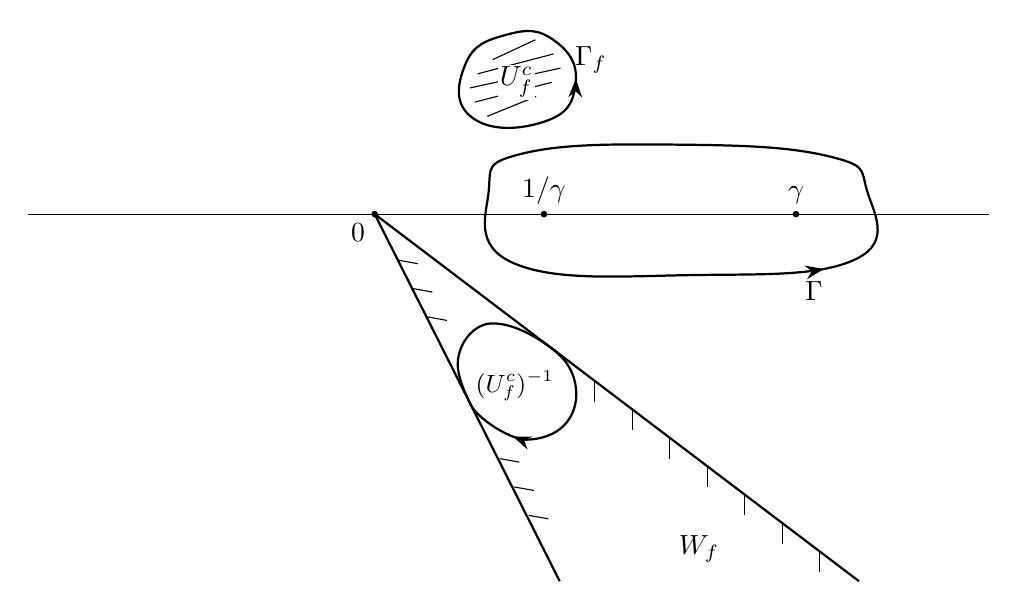
\begin{tikzpicture}[x=1cm,y=0.9cm,>=Stealth]
  % The real axis and the distinguished interval.
  \draw (-6.1,0)--(6.1,0);
  \coordinate (O) at (-1.7,0);
  \fill (O) circle (1.2pt) node[below left] {$0$};
  \fill (0.45,0) circle (1.2pt) node[above] {$1/\gamma$};
  \fill (3.65,0) circle (1.2pt) node[above] {$\gamma$};

  % A contour Gamma separating the interval from W_f.
  \draw[
    thick,
    postaction={decorate},
    decoration={markings,
      mark=at position 0.51 with {\arrowreversed{Stealth}}}
  ]
    plot[smooth cycle,tension=0.75] coordinates
      {(-0.25,0.34) (0.20,0.86) (2.15,0.98) (4.05,0.82)
       (4.55,0.34) (4.42,-0.63) (2.35,-0.86) (0.08,-0.70)};
  \node[below] at (3.88,-0.82) {$\Gamma$};

  % The neighbourhood U_f and its boundary Gamma_f.
  \draw[
    thick,
    postaction={decorate},
    decoration={markings,
      mark=at position 0.44 with {\arrowreversed{Stealth}}}
  ]
    plot[smooth cycle,tension=0.85] coordinates
      {(-0.46,1.36) (-0.55,2.11) (-0.03,2.53)
       (0.58,2.45) (0.85,1.83) (0.44,1.30)};
  \foreach \y/\xa/\xb in {1.52/-0.27/0.35,1.72/-0.43/0.55,
                            1.92/-0.49/0.66,2.12/-0.39/0.57,
                            2.32/-0.20/0.34}
    \draw[thin] (\xa,\y-0.14)--(\xb,\y+0.14);
  \node[fill=white,inner sep=0.8pt] at (0.10,1.86) {$U_f^c$};
  \node[right] at (0.72,2.17) {$\Gamma_f$};

  % The sector W_f and the inverse complementary component in it.
  \draw[thick] (O)--(0.65,-5.18);
  \draw[thick] (O)--(4.45,-5.18);
  \foreach \t in {0.65,1.05,1.45,3.45,3.85,4.25}
    \draw[thin] ({-1.7+0.46*\t},{-\t})--({-1.45+0.46*\t},{-\t-0.05});
  \foreach \t in {2.35,2.75,3.15,3.55,3.95,4.35,4.75}
    \draw[thin] ({-1.7+1.19*\t},{-\t})--({-1.70+1.19*\t},{-\t-0.30});
  % By (8.11), W_f is the radial hull of the inverse complementary
  % component.  Thus its two boundary rays support that component: the
  % curve is tangent to both rays (at opposite sides) but never crosses
  % either one.  The control handles at the two contact points are
  % parallel to the corresponding rays.
  \draw[
    thick,
    postaction={decorate},
    decoration={markings,
      mark=at position 0.59 with {\arrow{Stealth}}}
  ]
    (-0.28,-1.55)
      .. controls (0.00,-1.50) and (0.3405,-1.7187) .. (0.5558,-1.90)
      .. controls (0.7710,-2.0813) and (0.86,-2.30) .. (0.86,-2.55)
      .. controls (0.86,-2.80) and (0.72,-3.14) .. (0.28,-3.18)
      .. controls (0.05,-3.22) and (-0.3928,-2.8813) .. (-0.4751,-2.70)
      .. controls (-0.5573,-2.5187) and (-0.62,-2.35) .. (-0.64,-2.20)
      .. controls (-0.676,-1.93) and (-0.52,-1.62) .. cycle;
  \node at (0.08,-2.42) {\small $(U_f^c)^{-1}$};
  \node at (2.42,-4.73) {$W_f$};
\end{tikzpicture}
\end{center}

% Source PDF page 43 (printed page 42)
Take a simply closed smooth curve $\Gamma$ whose interior contains
$[1/\gamma,\gamma]$, and whose exterior contains $W_f$, and which
meets the half line $[0,\infty]$ only at two points.

\begin{lemma}\label{lem:8.5}
In the above situation, $f(\Delta)\mathfrak A^{\#}\subset\mathfrak A'$
and if $\xi$ is in $\mathfrak A^{\#}$, then
\begin{equation}
  (E_\gamma\eta)(f(\Delta)\xi)
  =\frac{i}{2\pi}\oint_\Gamma
  f(w^{-1}\Delta)\bigl[(R(w)E_\gamma\eta)\xi\bigr] \,dw
  \tag{8.12}\label{eq:8.12}
\end{equation}
for every $\eta\in\mathcal H$.
\end{lemma}

\begin{proof}
From the equality
\[
  E_\gamma=\frac{i}{2\pi}\oint_\Gamma R(w)E_\gamma\,dw,
\]
equality \eqref{eq:8.12} follows if $f$ is a constant function.
Considering the decomposition
$f(z)=f(z)-f(\infty)+f(\infty)$, we may assume that $f$ is in
$A[0,\infty]$.  Suppose $\xi$ is in $\mathfrak A^{\#}$.  By equality
\eqref{eq:8.8}, $R(w)\xi$ belongs to $\mathfrak A^{\#}$.
Furthermore, the inequality
\begin{align*}
 \|\pi'(R(w)\xi)\|
 &=\bigl\|w^{-1}\pi'\bigl(w^{-1}R(w^{-1})^T\xi-\xi\bigr)\bigr\|\\
 &\leq \frac{1}{|w|^2}\gamma(w^{-1})\|\pi(\xi)\|
      +\frac{1}{|w|}\|\pi'(\xi)\|
\end{align*}
implies that $\|\pi'(R(w)\xi)\|$ is uniformly bounded along the
curve $\Gamma_f$, so that $f(\Delta)\xi$ is $\pi'$-bounded because the
range of $(f(\Delta)-f(0)\,1)$ is contained in
$\mathcal D(\Delta^{-1})$ whenever $f$ is in $A[0,\infty]$.
Therefore, the first assertion follows.

In \Cref{lem:8.4}, fix $w_2$ on the curve $\Gamma_f$ and replace
$\xi_1$ and
% Source PDF page 44 (printed page 43)
$\xi_2$ by $E_\gamma\eta$ and $\xi$, respectively.  Then
\eqref{eq:8.7} turns out to be
\[
 (R(w_1)E_\gamma\eta)(R(w_2)\xi)
 =R(w_1w_2)\{w_1(R(w_1)E_\gamma\eta)\xi
 +(E_\gamma\eta)(\Delta R(w_2)\xi)\}.
\]
Multiplying by $i/(2\pi)$ on both sides and integrating with respect
to $w_1$ along the curve $\Gamma$, we get the left hand side
\[
 (E_\gamma\eta)(R(w_2)\xi)
 =\frac{i}{2\pi}\oint_\Gamma
 (R(w_1)E_\gamma\eta)(R(w_2)\xi)\,dw_1.
\]
Noticing that $w_1w_2\notin[0,\infty]$ for every $w_1\in\Gamma$ and
$w_2\in\Gamma_f$, we conclude that $R(w_1w_2)$ is an analytic
function of $w_1$ on and inside of the curve $\Gamma$, so that the
second term of the right hand side turns out to be
\[
 \frac{i}{2\pi}\oint_\Gamma
 R(w_1w_2)(E_\gamma\eta)(\Delta R(w_2)\xi)\,dw_1=0.
\]
Therefore, we have
\begin{equation}
 (E_\gamma\eta)(R(w_2)\xi)
 =\frac{i}{2\pi}\oint_\Gamma
 w_1R(w_1w_2)\bigl[(R(w_1)E_\gamma\eta)\xi\bigr] \,dw_1.
 \tag{8.13}\label{eq:8.13}
\end{equation}
Multiplying by $f(w_2)$ on both sides of \eqref{eq:8.13} and
integrating with respect to $w_2$ along the curve $\Gamma_f$, we get
\[
 (E_\gamma\eta)(f(\Delta)\xi)
 =-\frac{1}{(2\pi)^2}\oint_{\Gamma_f}\oint_\Gamma
 f(w_2)w_1R(w_1w_2)
 \bigl[(R(w_1)E_\gamma\eta)\xi\bigr] \,dw_1\,dw_2.
\]
Noticing that
% Source PDF page 45 (printed page 44)
\[
 f(w_1^{-1}t)=\frac{i}{2\pi}\oint_{\Gamma_f}
 f(w_2)w_1(t-w_1w_2)^{-1}\,dw_2
\]
for $w_1\in\Gamma$ and $t\in[0,\infty]$, we get
\[
 f(w_1^{-1}\Delta)=\frac{i}{2\pi}\oint_{\Gamma_f}
 f(w_2)w_1R(w_1w_2)\,dw_2;
\]
and then we get
\[
 (E_\gamma\eta)(f(\Delta)\xi)
 =\frac{i}{2\pi}\oint_\Gamma
 f(w^{-1}\Delta)\bigl[(R(w)E_\gamma\eta)\xi\bigr] \,dw,
\]
which completes the proof.
\end{proof}

\section{The One-Parameter Automorphisms defined by the Modular Operator
\texorpdfstring{$\Delta$}{Delta}}\label{sec:9}

Now, we are at the most crucial point in the proof of the fundamental
theorem of Tomita.  Consider the negative half line
\[
 W=\{z\in\widetilde{\mathbb C}:-z\in[0,\infty]\}.
\]
For each complex number $\alpha$, define an analytic function $z^\alpha$
on $\widetilde{\mathbb C}-W$ by
\[
 z^\alpha=\exp(\alpha\log|z|+i\alpha\arg z),
\]
where $-\pi<\arg z<\pi$.  Then we have
$z^{\alpha+\beta}=z^\alpha z^\beta$.  The normal operator
$\Delta^\alpha$ is given by
\begin{equation}
 \Delta^\alpha=\int_0^\infty z^\alpha\,dE(z)
 =\exp(\alpha\log\Delta).
 \tag{9.1}\label{eq:9.1}
\end{equation}
If $\alpha=s+it$ for $s,t\in\mathbb R$, we have
\[
  \Delta^\alpha=\Delta^s\Delta^{it};
\]
% Source PDF page 46 (printed page 45)
$\Delta^s$ is a positive self-adjoint operator and $\Delta^{it}$ is
unitary.

\begin{lemma}\label{lem:9.1}
For each complex number $\alpha$,
$\mathfrak A^{\#}\cap\mathcal D(\Delta^\alpha)$ is dense in the Hilbert
space $\mathcal D(\Delta^\alpha)$.
\end{lemma}

\begin{proof}
Let $\alpha=s+it$, $s,t\in\mathbb R$.  Take an integer
$n\geq |s|+1$ and consider the function
$f(z)=z^n(z^{2n}+1)^{-1}$.  We claim that
\[
  \Delta^{-1}f(\Delta^{-1})\mathfrak A^b
  \subset\mathfrak A^{\#}\cap\mathcal D(\Delta^\alpha).
\]
Indeed, if $\eta$ belongs to $\mathfrak A^b$, then $\eta$ and
$\Delta^{-1}\eta$ both belong to $\mathfrak A$, so that
$f(\Delta^{-1})\eta$ and $\Delta^{-1}f(\Delta^{-1})\eta$ both belong to
$\mathfrak A'$, because $f(z)$ and $zf(z)$ are both in
$A[0,\infty]$; hence
$\Delta^{-1}f(\Delta^{-1})\eta\in\mathfrak A^{\#}$.  By definition of
the function $f$, the range of $\Delta^{-1}f(\Delta^{-1})$ is
contained in $\mathcal D(\Delta^s)=\mathcal D(\Delta^\alpha)$.

Since
\[
 (1+\Delta^s)\Delta^{-1}f(\Delta^{-1})
 =\Delta^{n-1}(1+\Delta^s)(1+\Delta^{2n})^{-1}
\]
is a bounded self-adjoint operator with dense range in $\mathcal H$,
and $\mathfrak A^b$ is dense in $\mathcal H$,
$(1+\Delta^s)\Delta^{-1}f(\Delta^{-1})\mathfrak A^b$ is dense in
$\mathcal H$; therefore by \hyperref[lem:1.1]{Lemma~1.1},
$\Delta^{-1}f(\Delta^{-1})\mathfrak A^b$ is dense in the Hilbert space
$\mathcal D(\Delta^s)=\mathcal D(\Delta^\alpha)$, so that
$\mathfrak A^{\#}\cap\mathcal D(\Delta^\alpha)$ is dense in
$\mathcal D(\Delta^\alpha)$.
\end{proof}

\begin{theorem}\label{thm:9.1}
For each $\xi\in\mathfrak A\cap\mathcal D(\Delta^{-\alpha})$ and
$\eta\in\mathfrak A'\cap\mathcal D(\Delta^\alpha)$,
$(\Delta^{-\alpha}\xi)\eta$ belongs to
$\mathcal D(\Delta^\alpha)$ and satisfies the formula
\begin{equation}
 \Delta^\alpha\bigl((\Delta^{-\alpha}\xi)\eta\bigr)
 =\xi(\Delta^\alpha\eta).
 \tag{9.2}\label{eq:9.2}
\end{equation}
\end{theorem}

\begin{proof}
Consider the function
\begin{equation}
 f_\delta(z)=\left(\frac{z+\delta}{1+\delta z}\right)^\alpha,
 \qquad 0\leq\delta\leq1.
 \tag{9.3}\label{eq:9.3}
\end{equation}
% Source PDF page 47 (printed page 46)
Then $f_0(z)=z^\alpha$.  If $0<\delta\leq1$, then $f_\delta$ is
analytic except on the segment $-1/\delta\leq z\leq-\delta$.  Hence
$f_\delta$ is analytic in a neighborhood of $[0,\infty]$ and we may
assume that the set $W_{f_\delta}$ defined by \eqref{eq:8.11} is
contained in the left half plane $\operatorname{Re}z\leq0$.  Now we
shall apply \Cref{lem:8.5} to $f_\delta$.  Take a simply closed smooth
curve $\Gamma$ as in the proof of \Cref{lem:8.5}, so we have the
following picture:
\begin{center}
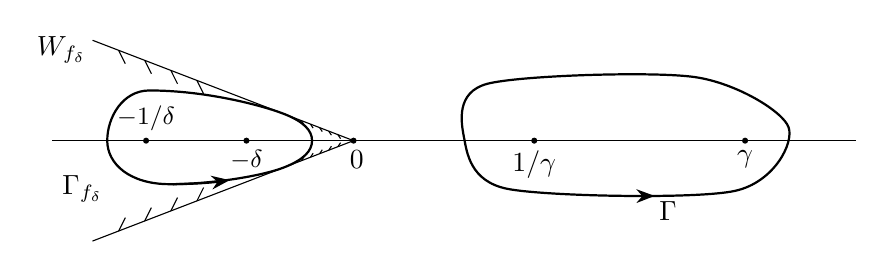
\begin{tikzpicture}[x=0.85cm,y=0.85cm,>=Stealth]
  \draw (-6,0)--(6,0);
  \draw (-5.4,1.5)--(-1.5,0)--(-5.4,-1.5);
  \foreach \t in {0.10,0.20,0.30,0.40} {
    \draw[thin] ({-5.4+3.9*\t},{1.5-1.5*\t})--
                ({-5.30+3.9*\t},{1.30-1.5*\t});
    \draw[thin] ({-5.4+3.9*\t},{-1.5+1.5*\t})--
                ({-5.30+3.9*\t},{-1.30+1.5*\t});
  }
  % Shorten the hatching toward the vertex so that the upper and lower
  % strokes stay on their own sides of the real axis.
  \foreach \t in {0.80,0.835,0.87,0.905,0.94} {
    \draw[thin] ({-5.4+3.9*\t},{1.5-1.5*\t})--
                ({-5.36+3.9*\t},{1.44-1.5*\t});
    \draw[thin] ({-5.4+3.9*\t},{-1.5+1.5*\t})--
                ({-5.36+3.9*\t},{-1.44+1.5*\t});
  }
  \node[left] at (-5.35,1.35) {$W_{f_\delta}$};
  % The singular interval is invariant under inversion.  Hence the
  % extreme arguments of Gamma_{f_delta} generate the two boundary rays
  % of W_{f_delta}: the contour is tangent to both rays but does not cross
  % either one.
  \draw[thick]
    (-2.12,0.00)
      .. controls (-2.12,0.15) and (-2.238,0.283846) .. (-2.55,0.403846)
      .. controls (-2.862,0.523846) and (-3.70,0.75) .. (-4.55,0.75)
      .. controls (-4.95,0.75) and (-5.18,0.35) .. (-5.18,0.00)
      .. controls (-5.18,-0.35) and (-4.84,-0.65) .. (-4.25,-0.65)
      .. controls (-3.60,-0.65) and (-2.862,-0.523846) .. (-2.55,-0.403846)
      .. controls (-2.238,-0.283846) and (-2.12,-0.15) .. cycle;
  \draw[->,thick] (-4.20,-0.65)..controls (-3.95,-0.65) and (-3.65,-0.63)..(-3.35,-0.59);
  \fill (-4.6,0) circle (1.1pt);
  \fill (-3.10,0) circle (1.1pt);
  \node[above,font=\small] at (-4.6,0) {$-1/\delta$};
  \node[below,font=\small] at (-3.10,0) {$-\delta$};
  \node[left] at (-5.10,-0.72) {$\Gamma_{f_\delta}$};
  % Put the direction mark on Gamma itself; a detached auxiliary stroke
  % would incorrectly suggest a second curve below the contour.
  \draw[
    thick,
    postaction={decorate},
    decoration={markings,
      mark=at position 0.63 with {\arrowreversed{Stealth}}}
  ] plot[smooth cycle] coordinates
    {(0.15,0.05) (0.5,0.85) (3.6,0.95) (5.0,0.2)
     (4.2,-0.75) (0.8,-0.72)};
  \fill (1.2,0) circle (1.1pt);
  \fill (4.35,0) circle (1.1pt);
  \fill (-1.5,0) circle (1.1pt);
  \node[below] at (1.2,0) {$1/\gamma$};
  \node[below] at (4.35,0) {$\gamma$};
  \node[below] at (3.2,-0.76) {$\Gamma$};
  \node[below] at (-1.45,0) {$0$};
\end{tikzpicture}
\end{center}

Take $\eta_1$ and $\eta_2$ in $\mathfrak A^{\#}$ and $\xi$ in
$\mathfrak A$.  Since $E_\gamma\xi$\ednote{The source prints
$E_\gamma\eta$ here; this has been corrected to $E_\gamma\xi$, consistently
with the following expression.} belongs to
$\mathcal D(\Delta^{1/2})=\mathcal D^{\#}$,
$(E_\gamma\xi)^{\#}$ is defined.  By \Cref{lem:8.5}, we get
\begin{align*}
 &(f_\delta(\Delta)\eta_1\mid(E_\gamma\xi)^{\#}\eta_2)
   =((E_\gamma\xi)(f_\delta(\Delta)\eta_1)\mid\eta_2)\\
 &\quad=\frac{i}{2\pi}\oint_\Gamma
   \bigl(f_\delta(w^{-1}\Delta)[(R(w)E_\gamma\xi)\eta_1]
   \mid\eta_2\bigr)\,dw\\
 &\quad=\frac{i}{2\pi}\oint_\Gamma
   \bigl((R(w)E_\gamma\xi)\eta_1
   \mid f_\delta(w^{-1}\Delta)^*\eta_2\bigr)\,dw\\
 &\quad=\frac{i}{2\pi}\oint_\Gamma
   \bigl(\eta_1\mid(R(w)E_\gamma\xi)^{\#}
   (f_\delta(w^{-1}\Delta)^*\eta_2)\bigr)\,dw,
\end{align*}
where the last step of the above calculation is justified as follows:
the function
\[
 z\longmapsto(w\overline\delta+z)^{\overline\alpha}
 (\overline w+\delta z)^{-\overline\alpha}
\]
is analytic in a neighborhood of $[0,\infty]$ and
\[
 f_\delta(w^{-1}\Delta)^*
 =(w\overline\delta+\Delta)^{\overline\alpha}
  (\overline w+\delta\Delta)^{-\overline\alpha};
\]
hence \Cref{lem:8.5} assures that
$f_\delta(w^{-1}\Delta)^*\eta_2$ is in $\mathfrak A'$, and also
$R(w)E_\gamma\xi$ belongs to $\mathcal D^{\#}$.  Therefore, we get
% Source PDF page 48 (printed page 47)
\begin{equation}
 (f_\delta(\Delta)\eta_1\mid(E_\gamma\xi)^{\#}\eta_2)
 =\frac{i}{2\pi}\oint_\Gamma
 \bigl(\eta_1\mid(R(w)E_\gamma\xi)^{\#}
 (f_\delta(w^{-1}\Delta)^*\eta_2)\bigr)\,dw
 \tag{9.4}\label{eq:9.4}
\end{equation}
for each $\xi\in\mathfrak A$ and
$\eta_1,\eta_2\in\mathfrak A^{\#}$.

Since
\[
 f_\delta(w^{-1}\Delta)^*
 =(1+\overline w\delta\Delta^{-1})^{\overline\alpha}
  (\delta+\overline w\Delta^{-1})^{-\overline\alpha},
\]
if we define a function $g_\delta^w$ by
\[
 g_\delta^w(z)
 =\left(\frac{1+\overline w\delta z}
 {\delta+\overline w z}\right)^{\overline\alpha}
 -\delta^{\overline\alpha},
\]
then
\[
 f_\delta(w^{-1}\Delta)^*
 =g_\delta^w(\Delta^{-1})+\delta^{\overline\alpha}\,1
\]
and $g_\delta^w$ belongs to $A[0,\infty]$.  Hence by
\eqref{eq:8.5-prime}, we have
\[
 \|\pi'(f_\delta(w^{-1}\Delta)^*\eta_2)\|
 \leq |\delta^{\overline\alpha}|\|\pi'(\eta_2)\|
 +\frac{1}{2\pi}\ell
 \sup_{z\in\Gamma_{f_\delta}}
 \bigl(\gamma(z)|g_\delta^w(z)|\bigr)\|\pi(\eta_2)\|,
\]
where $\Gamma_{f_\delta}$ denotes a simply closed smooth curve with
length $\ell$, whose interior contains the segment
$[-1/\delta,-\delta]$.  Hence there exists a constant $\gamma_0$ not
depending on $w$ such that
\[
 \|\pi'(f_\delta(w^{-1}\Delta)^*\eta_2)\|\leq\gamma_0.
\]
The operator $\xi\mapsto(E_\gamma\xi)^{\#}$ is bounded, so that the
function $w\mapsto(R(w)E_\gamma\xi)^{\#}$ is continuous on $\Gamma$;
hence the function
\[
 w\in\Gamma\longmapsto
 (R(w)E_\gamma\xi)^{\#}
 (f_\delta(w^{-1}\Delta)^*\eta_2)\in\mathcal H
\]
is bounded on $\Gamma$.  Thus both sides of equality \eqref{eq:9.4}
are continuous functions of $\eta_1$, so that equality \eqref{eq:9.4}
remains true for every $\eta_1\in\mathcal H$.  Thus we get
% Source PDF page 49 (printed page 48)
\begin{equation}
 (f_\delta(\Delta)\eta_1\mid(E_\gamma\xi)^{\#}\eta_2)
 =\frac{i}{2\pi}\oint_\Gamma
 \bigl((R(w)E_\gamma\xi)\eta_1
 \mid f_\delta(w^{-1}\Delta)^*\eta_2\bigr)\,dw
 \tag{9.5}\label{eq:9.5}
\end{equation}
for $\eta_1\in\mathfrak A'\cap\mathcal D(\Delta^\alpha)$,
$\eta_2\in\mathfrak A^{\#}\cap\mathcal D(\Delta^\alpha)$, and
$\xi\in\mathfrak A\cap\mathcal D(\Delta^{-\alpha})$.

We shall show that equality \eqref{eq:9.5} is also true in the case
when $\delta=0$.  Write $\alpha=s+it$ and put
\[
 \gamma_1=\inf\{\operatorname{Re}w:\overline w\in\Gamma\},
 \qquad
 \gamma_2=\sup\{|w|:w\in\Gamma\},
\]
\[
 \gamma_3=\sup\{|\arg w|:\overline w\in\Gamma\},
 \qquad
 \gamma_4=\exp(\gamma_3|t|).
\]
For each $w\in\Gamma$ and $\lambda\in[0,\infty]$, we have
\begin{align*}
 |f_\delta(w^{-1}\lambda)|
 &=\left|\left(\frac{\lambda+w\delta}
 {w+\delta\lambda}\right)^\alpha\right|\\
 &=\left|\frac{\lambda+w\delta}{w+\delta\lambda}\right|^s
 \exp\left\{-t\arg\left(\frac{\lambda+w\delta}
 {w+\delta\lambda}\right)\right\}\\
 &=\left|\frac{\lambda+w\delta}{w+\delta\lambda}\right|^s
 \exp\{t(\arg(w+\delta\lambda)-\arg(\lambda+w\delta))\}.
\end{align*}
Since $\operatorname{Re}w>0$ and $\lambda$ is real, we have
\[
 |\arg(w+\delta\lambda)-\arg(\lambda+w\delta)|\leq|\arg w|,
\]
and then
\[
 \exp\{t(\arg(w+\delta\lambda)-\arg(\lambda+w\delta))\}
 \leq\exp(\gamma_3|t|)\leq\gamma_4.
\]
If $s>0$, then since $|1+\delta w^{-1}\lambda|\geq1$, we have
% Source PDF page 50 (printed page 49)
\begin{align*}
 \left|\frac{\lambda+w\delta}{w+\delta\lambda}\right|^s
 &\leq|w^{-1}\lambda+\delta|^s
 \leq(|w|^{-1}\lambda+\delta)^s\\
 &\leq(\gamma_1^{-1}\lambda+\delta)^s
 \leq(\gamma_1^{-1}\lambda+1)^s.
\end{align*}
Noticing that
$\mathcal D(\Delta^s)=\mathcal D((\gamma_1^{-1}\Delta+1)^s)$, we
have, for each $\eta\in\mathcal D(\Delta^s)$,
\[
 \|f_\delta(w^{-1}\Delta)^*\eta\|
 \leq\gamma_4\|(\gamma_1^{-1}\Delta+1)^s\eta\|.
\]
If $s<0$, then we have
\begin{align*}
 \left|\frac{\lambda+w\delta}{w+\delta\lambda}\right|^s
 &=\left|\frac{1+\lambda^{-1}w\delta}
 {\lambda^{-1}w+\delta}\right|^s
 \leq|\lambda^{-1}w+\delta|^{-s}\\
 &\leq(\gamma_2\lambda^{-1}+\delta)^{-s}
 \leq(\gamma_2\lambda^{-1}+1)^{-s}.
\end{align*}
Noticing again that
$\mathcal D(\Delta^s)=\mathcal D((\gamma_2\Delta^{-1}+1)^{-s})$, we
have
\[
 \|f_\delta(w^{-1}\Delta)^*\eta\|
 \leq\gamma_4\|(\gamma_2\Delta^{-1}+1)^{-s}\eta\|,
 \qquad \eta\in\mathcal D(\Delta^s).
\]
If $s=0$, then
\[
 \|f_\delta(w^{-1}\Delta)^*\eta\|\leq\gamma_4\|\eta\|.
\]
Since $\eta_2$ belongs to
$\mathcal D(\Delta^\alpha)=\mathcal D(\Delta^s)$, for every
$\varepsilon>0$ we can find a $\lambda_0>1$ such that
\[
 \gamma_4\|(\gamma_1^{-1}\Delta+1)^s(1-E_{\lambda_0})\eta_2\|
 <\varepsilon\|\eta_2\|
\]
in the case when $s>0$, or
\[
 \gamma_4\|(\gamma_2\Delta^{-1}+1)^{-s}(1-E_{\lambda_0})\eta_2\|
 <\varepsilon\|\eta_2\|
\]
in the case when $s\leq0$.  Hence we have
% Source PDF page 51 (printed page 50)
\[
 \|f_\delta(w^{-1}\Delta)^*(1-E_{\lambda_0})\eta_2\|
 <\varepsilon\|\eta_2\|.
\]
Remark that the number $\lambda_0>0$, hence the projection
$E_{\lambda_0}$, depends on neither $w\in\Gamma$ nor $\delta<1$.
Since $\overline{f_\delta}(\overline w^{-1}\lambda)$ converges to
$\overline{f_0}(\overline w^{-1}\lambda)$ uniformly for
$\lambda\in[1/\lambda_0,\lambda_0]$ and $w\in\Gamma$ as $\delta$
tends to zero, we have
\[
 \sup_{w\in\Gamma}
 \|f_\delta(w^{-1}\Delta)^*E_{\lambda_0}\eta_2
 -\overline w^{-\overline\alpha}\Delta^{\overline\alpha}
 E_{\lambda_0}\eta_2\|
 \leq\varepsilon\|\eta_2\|
\]
for a sufficiently small $\delta>0$.  Thus we conclude that
\[
 \lim_{\delta\to0}\sup_{w\in\Gamma}
 \|f_\delta(w^{-1}\Delta)^*\eta_2
 -\overline w^{-\overline\alpha}\Delta^{\overline\alpha}\eta_2\|=0
\]
for each $\eta_2\in\mathcal D(\Delta^\alpha)$.  Of course, it is an
immediate consequence of the above discussion that
\[
 \lim_{\delta\to0}\|f_\delta(\Delta)\eta_1
 -\Delta^\alpha\eta_1\|=0
\]
for each $\eta_1\in\mathcal D(\Delta^\alpha)$.  Therefore, equality
\eqref{eq:9.5} turns out, by taking limits, to be
\begin{equation}
 (\Delta^\alpha\eta_1\mid(E_\gamma\xi)^{\#}\eta_2)
 =\frac{i}{2\pi}\oint_\Gamma
 \bigl((R(w)E_\gamma\xi)\eta_1
 \mid\overline w^{-\overline\alpha}
 \Delta^{\overline\alpha}\eta_2\bigr)\,dw
 \tag{9.6}\label{eq:9.6}
\end{equation}
for each $\eta_1\in\mathfrak A'\cap\mathcal D(\Delta^\alpha)$,
$\eta_2\in\mathfrak A^{\#}\cap\mathcal D(\Delta^\alpha)$, and
$\xi\in\mathfrak A\cap\mathcal D(\Delta^{-\alpha})$.  The right hand
side of \eqref{eq:9.6} equals
\[
 \frac{i}{2\pi}\oint_\Gamma
 \bigl(w^{-\alpha}(R(w)E_\gamma\xi)\eta_1
 \mid\Delta^{\overline\alpha}\eta_2\bigr)\,dw
 =\bigl((\Delta^{-\alpha}E_\gamma\xi)\eta_1
 \mid\Delta^{\overline\alpha}\eta_2\bigr).
\]
Hence we get
% Source PDF page 52 (printed page 51)
\[
 (\Delta^\alpha\eta_1\mid(E_\gamma\xi)^{\#}\eta_2)
 =\bigl((\Delta^{-\alpha}E_\gamma\xi)\eta_1
 \mid\Delta^{\overline\alpha}\eta_2\bigr).
\]
Since we have by \eqref{eq:8.9}
\[
 (E_\gamma\xi)^{\#}=SE_\gamma\xi
 =\Delta^{-1/2}JE_\gamma\xi
 =\Delta^{-1/2}E_\gamma^TJ\xi
 =E_\gamma\Delta^{-1/2}J\xi=E_\gamma\xi^{\#},
\]
we have
\[
 \lim_{\gamma\to\infty}(E_\gamma\xi)^{\#}=\xi^{\#}.
\]
Recalling that $\eta_2$ is in $\mathfrak A'$, we get
\[
 \lim_{\gamma\to\infty}(E_\gamma\xi)^{\#}\eta_2
 =\xi^{\#}\eta_2.
\]
Since $\xi$ belongs to $\mathcal D(\Delta^{-\alpha})$, we have
\[
 \lim_{\gamma\to\infty}(\Delta^{-\alpha}E_\gamma\xi)
 =\Delta^{-\alpha}\xi;
\]
\[
 \lim_{\gamma\to\infty}(\Delta^{-\alpha}E_\gamma\xi)\eta_1
 =(\Delta^{-\alpha}\xi)\eta_1
\]
because $\eta_1$ belongs to $\mathfrak A'$.  Therefore, we have
\begin{align}
 ((\Delta^{-\alpha}\xi)\eta_1\mid
  \Delta^{\overline\alpha}\eta_2)
 &= (\Delta^\alpha\eta_1\mid\xi^{\#}\eta_2)\notag\\
 &= (\xi(\Delta^\alpha\eta_1)\mid\eta_2).
 \tag{9.7}\label{eq:9.7}
\end{align}
By \Cref{lem:9.1},
$\mathfrak A^{\#}\cap\mathcal D(\Delta^\alpha)$ is dense in the
Hilbert space $\mathcal D(\Delta^\alpha)$, so that equality
\eqref{eq:9.7} implies that $(\Delta^{-\alpha}\xi)\eta_1$ belongs to
$\mathcal D(\Delta^\alpha)$ and that
\[
 \Delta^\alpha\bigl((\Delta^{-\alpha}\xi)\eta_1\bigr)
 =\xi(\Delta^\alpha\eta_1)
\]
% Source PDF page 53 (printed page 52)
for each $\xi\in\mathfrak A\cap\mathcal D(\Delta^{-\alpha})$ and
$\eta_1\in\mathfrak A'\cap\mathcal D(\Delta^\alpha)$.  This completes
the proof.
\end{proof}

\begin{corollary}\label{cor:9.1}
$\Delta^{it}$, $-\infty<t<\infty$, form a one-parameter automorphism
group of $\mathfrak A$ and
\begin{equation}
 \pi(\Delta^{it}\xi)=\Delta^{it}\pi(\xi)\Delta^{-it},
 \qquad \xi\in\mathfrak A.
 \tag{9.8}\label{eq:9.8}
\end{equation}
\end{corollary}

\begin{proof}
Noticing that
$\mathcal D(\Delta^{it})=\mathcal D(\Delta^{-it})=\mathcal H$, we get
\[
 \Delta^{it}\bigl(\xi(\Delta^{-it}\eta)\bigr)
 =(\Delta^{it}\xi)\eta,
 \qquad \xi\in\mathfrak A,\quad\eta\in\mathfrak A'.
\]
Hence we have
$\pi(\Delta^{it}\xi)=\Delta^{it}\pi(\xi)\Delta^{-it}$.  Of course,
$\Delta^{it}\xi$ is $\pi$-bounded.  This completes the proof.
\end{proof}

Therefore, the one-parameter unitary group $\{\Delta^{it}\}$ induces
a one-parameter $*$-automorphism group of the left von Neumann algebra
$\mathcal L(\mathfrak A)$ of $\mathfrak A$.

\section{Formulation of the Modular Hilbert Algebra}\label{sec:10}

Now, we are at the final stage of the construction of the modular
Hilbert algebra equivalent to a given generalized Hilbert algebra.
Throughout this section, we suppose $\mathfrak A$ is an achieved
generalized Hilbert algebra.

\begin{lemma}\label{lem:10.1}
If $f$ is a continuous positive definite function of a real variable,
then $f(\log\Delta)$ carries $\mathfrak A$ into $\mathfrak A$ and
\begin{equation}
 (f(\log\Delta)\xi)^{\#}=f(\log\Delta)\xi^{\#},
 \qquad \xi\in\mathfrak A.
 \tag{10.1}\label{eq:10.1}
\end{equation}
\end{lemma}

% Source PDF page 54 (printed page 53)
\begin{proof}
By Bochner's Theorem, $f$ is represented by an integral
\[
  f(\lambda)=\int_{-\infty}^{\infty}e^{i\lambda t}\,d\mu(t),
\]
where $\mu$ is a finite positive measure.  Hence we have
\[
  f(\log\Delta)=\int_{-\infty}^{\infty}\Delta^{it}\,d\mu(t),
\]
where the integral is taken in the strong operator topology.
Therefore, for each $\xi\in\mathfrak A$ and
$\eta\in\mathfrak A'$, we have
\begin{align*}
 \|(f(\log\Delta)\xi)\eta\|
 &=\left\|\int_{-\infty}^{\infty}(\Delta^{it}\xi)\eta\,d\mu(t)\right\|\\
 &\leq\int_{-\infty}^{\infty}\|(\Delta^{it}\xi)\eta\|\,d\mu(t)\\
 &\leq\int_{-\infty}^{\infty}\|\pi(\xi)\|\,\|\eta\|\,d\mu(t)
 =f(0)\|\pi(\xi)\|\,\|\eta\|,
\end{align*}
so that $f(\log\Delta)\xi$ belongs to $\mathfrak A$, because
$f(\log\Delta)$ leaves the domain $\mathcal D(\Delta^{1/2})$
invariant.  For each $\xi\in\mathfrak A$, we have
\begin{align*}
 (f(\log\Delta)\xi)^{\#}
 &=Sf(\log\Delta)\xi
 =\Delta^{-1/2}Jf(\log\Delta)\xi\\
 &=\Delta^{-1/2}\overline f(\log\Delta^{-1})J\xi
 =\Delta^{-1/2}\overline f(-\log\Delta)J\xi\\
 &=\Delta^{-1/2}f(\log\Delta)J\xi
 =f(\log\Delta)\Delta^{-1/2}J\xi\\
 &=f(\log\Delta)\xi^{\#}.
\end{align*}
\end{proof}

% Source PDF page 55 (printed page 54)
Now, Tomita's fundamental theorem is at hand as follows:

\begin{theorem}\label{thm:10.1}
For every generalized Hilbert algebra $\mathfrak A$, there exists a
modular Hilbert algebra $\mathfrak B$ which is equivalent to
$\mathfrak A$.  Therefore, there is an isometric involution $J$ of the
Hilbert space $\mathcal H$, which is the completion of $\mathfrak A$,
such that
\begin{equation}
  J\mathcal L(\mathfrak A)J=\mathcal L(\mathfrak A)'.
  \tag{10.2}\label{eq:10.2}
\end{equation}
In particular, the left von Neumann algebra $\mathcal L(\mathfrak A)$
of $\mathfrak A$ is anti-isomorphic to its commutant
$\mathcal L(\mathfrak A)'$.
\end{theorem}

\begin{proof}
We may assume that $\mathfrak A$ is achieved.  Keep the notation as
before.  Let $\mathcal E$ denote the linear space spanned by $f*g$,
where $f$ and $g$ are continuous functions of real variables with
compact support and
\[
  f*g(t)=\int_{-\infty}^{\infty}f(s)g(t-s)\,ds.
\]
For each function $f$ of a real variable, put
$\widetilde f(t)=\overline{f(-t)}$.  Putting
$e_\alpha(t)=e^{\alpha t}$ for each complex number $\alpha$, we have
\[
  e_\alpha(f*g)=(e_\alpha f)*(e_\alpha g),
\]
so that the map $f\mapsto e_\alpha f$ carries $\mathcal E$ onto
$\mathcal E$.  Let $\mathfrak B$ be the subalgebra of $\mathfrak A$
generated algebraically by $f(\log\Delta)\xi$,
$f\in\mathcal E$ and $\xi\in\mathfrak A$.  Since
\[
  (f(\log\Delta)\xi)^{\#}
  =\widetilde f(\log\Delta)\xi^{\#},
\]
$\mathfrak B$ is a self-adjoint subalgebra of $\mathfrak A$.  By the
equality
% Source PDF page 56 (printed page 55)
\begin{align*}
 \Delta^\alpha f(\log\Delta)\xi
 &=e_\alpha(\log\Delta)f(\log\Delta)\xi\\
 &=(e_\alpha f)(\log\Delta)\xi,
\end{align*}
$\mathfrak B$ is invariant under the operator $\Delta^\alpha$.

To complete the proof, we shall show that $\mathfrak B$ is dense in
the Hilbert space $\mathcal D(\Delta^\alpha)$.  Put
$\alpha=s+it$.  Take an arbitrary $\xi$ in
$\mathcal D(\Delta^\alpha)$ and $\varepsilon>0$.  Then there exists a
continuous function $f$ with compact support such that
\[
  \|(1+\Delta^s)(f(\log\Delta)\xi-\xi)\|<\varepsilon.
\]
We can find a sequence $\{f_n\}$ in $\mathcal E$ such that
$\{f_n\}$ converges to $f$ uniformly and $\operatorname{supp}f_n$ is
contained in a fixed compact set $K$ in $\mathbb R$.  Let $\chi_K$ be
the characteristic function of $K$.  Then
$(1+\Delta^s)\chi_K(\log\Delta)$ is bounded and
\[
  (1+\Delta^s)f_n(\log\Delta)\xi
  =(1+\Delta^s)\chi_K(\log\Delta)f_n(\log\Delta)\xi.
\]
Hence we have
\[
  \lim_{n\to\infty}
  \|(1+\Delta^s)(f_n(\log\Delta)\xi-f(\log\Delta)\xi)\|=0.
\]
Hence we can find a function $f_0$ in $\mathcal E$ such that
\[
  \|(1+\Delta^s)(f_0(\log\Delta)\xi-\xi)\|<\varepsilon,
\]
which means by \hyperref[lem:1.1]{Lemma~1.1} that $\mathfrak B$ is
dense in $\mathcal D(\Delta^\alpha)$.  In particular, $\mathfrak B$
is dense in $\mathcal D(\Delta^{1/2})$, so that
$\mathfrak B''=\mathfrak A$ and $\mathfrak B'=\mathfrak A'$ by
\hyperref[lem:5.2]{Lemma~5.2}.  Therefore, $\mathfrak B$ satisfies all
postulates for a modular Hilbert algebra, except possibly postulate
(VII), and is equivalent to $\mathfrak A$.

Now we shall show that the function
$\alpha\mapsto(\Delta^\alpha\xi\mid\eta)$,
$\xi,\eta\in\mathfrak B$, is
% Source PDF page 57 (printed page 56)
analytic.  Consider the set $\mathfrak C$ of all elements $\xi$ with
the following properties:
\begin{enumerate}[label=(\alph*)]
 \item $\xi$ is in $\bigcap_\alpha\mathcal D(\Delta^\alpha)$;
 \item $\Delta^\alpha\xi$ is in $\mathfrak A^{\#}$ for every complex
 number $\alpha$;
 \item the function $\alpha\mapsto(\Delta^\alpha\xi\mid\eta)$ is
 analytic for each $\eta\in\mathfrak A$.
\end{enumerate}
Then $\mathfrak C$ clearly contains all elements of the form
$f(\log\Delta)\xi$, $f\in\mathcal E$ and $\xi\in\mathfrak A$.  We
shall show that $\mathfrak C$ is an algebra.  Take $\xi_1$ and
$\xi_2$ in $\mathfrak C$ and $\eta\in\mathfrak A$.  Then we have
\begin{align*}
 &\frac1h\{(\Delta^{\alpha+h}(\xi_1\xi_2)\mid\eta)
 -(\Delta^\alpha(\xi_1\xi_2)\mid\eta)\}\\
 &\quad=\frac1h\bigl(\{(\Delta^{\alpha+h}\xi_1)
   (\Delta^{\alpha+h}\xi_2)
  -(\Delta^\alpha\xi_1)(\Delta^\alpha\xi_2)\}\mid\eta\bigr)\\
 &\quad=\frac1h\bigl((\Delta^{\alpha+h}\xi_1-\Delta^\alpha\xi_1)
       \Delta^{\alpha+h}\xi_2\mid\eta\bigr)
  +\frac1h\bigl((\Delta^\alpha\xi_1)
       (\Delta^{\alpha+h}\xi_2-\Delta^\alpha\xi_2)\mid\eta\bigr)\\
 &\quad=\frac1h\bigl(\Delta^{\alpha+h}\xi_1-\Delta^\alpha\xi_1
       \mid\eta(\Delta^{\alpha+h}\xi_2)^b\bigr)
  +\frac1h\bigl(\Delta^{\alpha+h}\xi_2-\Delta^\alpha\xi_2
       \mid(\Delta^\alpha\xi_1)^{\#}\eta\bigr)\\
 &\quad=\frac1h\bigl(\Delta^{\alpha+h}\xi_1-\Delta^\alpha\xi_1
       \mid\eta(J\Delta^{\overline\alpha-1/2+\overline h}\xi_2)\bigr)
  +\frac1h\bigl(\Delta^{\alpha+h}\xi_2-\Delta^\alpha\xi_2
       \mid(\Delta^\alpha\xi_1)^{\#}\eta\bigr).
\end{align*}
As in the proof of \hyperref[lem:2.1]{Lemma~2.1}, the functions
$\alpha\mapsto\Delta^\alpha\xi_i$, $i=1,2$, are strongly analytic, so
that $\Delta^{\overline\alpha-1/2+\overline h}\xi_2$ converges to
$\Delta^{\overline\alpha-1/2}\xi_2$ as $h$ tends to $0$; hence the
function $\alpha\mapsto(\Delta^\alpha(\xi_1\xi_2)\mid\eta)$ is
analytic.  Hence $\xi_1\xi_2$ satisfies condition (c) as well as
conditions (a) and (b), which means that $\mathfrak C$ is an algebra
as desired.  Therefore $\mathfrak C$ contains $\mathfrak B$.  This
completes the proof.
\end{proof}

\begin{corollary}\label{cor:10.1}
If $\mathfrak A$ is a generalized Hilbert algebra, then we have
% Source PDF page 58 (printed page 57)
\begin{equation}
  J\mathfrak A''=\mathfrak A'
  \qquad\text{and}\qquad
  J\mathfrak A'=\mathfrak A''.
  \tag{10.3}\label{eq:10.3}
\end{equation}
\end{corollary}

\begin{proof}
Let $\mathfrak A_0$ be a modular Hilbert algebra in $\mathfrak A''$
constructed in \Cref{thm:10.1}.  Then we have, for each pair
$\xi,\eta$ in $\mathfrak A_0$,
\[
  J(\xi\eta)=(J\eta)(J\xi).
\]
Take an arbitrary $\eta\in\mathfrak A'$.  Then we can choose a
sequence $\{\eta_n\}$ in $\mathfrak A_0$ with
$\eta=\lim_{n\to\infty}\eta_n$, so that we have for each
$\xi\in\mathfrak A_0$,
\begin{align*}
 (J\eta)(J\xi)
 &=\pi'(J\xi)J\eta
   =\lim_{n\to\infty}\pi'(J\xi)J\eta_n\\
 &=\lim_{n\to\infty}J(\xi\eta_n)
   =\lim_{n\to\infty}J\pi(\xi)\eta_n\\
 &=J\pi(\xi)\eta=J(\xi\eta).
\end{align*}
Hence we have
\[
  \|(J\eta)(J\xi)\|\leq\|\pi'(\eta)\|\,\|\xi\|.
\]
Therefore, recalling that $J\mathfrak A'\subset\mathcal D^{\#}$, we
can conclude that $J\eta$ belongs to $\mathfrak A''$.  Thus we get
$J\mathfrak A'=\mathfrak A''$.  By symmetry, we also have
$J\mathfrak A''=\mathfrak A'$.
\end{proof}

\section{Tensor Product and Direct Sum of Modular Hilbert Algebras}
\label{sec:11}

Let $\mathfrak A_1$ and $\mathfrak A_2$ be two modular Hilbert
algebras.  Let $\mathcal H_1$ and $\mathcal H_2$ be their completions
respectively.  Let $\mathfrak A_1\otimes\mathfrak A_2=\mathfrak A$ be
the algebraic tensor product of $\mathfrak A_1$ and
$\mathfrak A_2$.  Then $\mathfrak A_1\otimes\mathfrak A_2$ has the
natural involutive algebra structure defined by
% Source PDF page 59 (printed page 58)
\[
 (\xi_1\otimes\xi_2)(\eta_1\otimes\eta_2)
 =\xi_1\eta_1\otimes\xi_2\eta_2,
\]
\[
 (\xi_1\otimes\xi_2)^{\#}
 =\xi_1^{\#}\otimes\xi_2^{\#}.
\]
Also $\mathfrak A_1\otimes\mathfrak A_2$ has the inner product defined
by
\[
 (\xi_1\otimes\xi_2\mid\eta_1\otimes\eta_2)
 =(\xi_1\mid\eta_1)(\xi_2\mid\eta_2).
\]
Let $\mathcal H$ be the completion of $\mathfrak A$.  Then
$\mathcal H$ is nothing but the tensor product
$\mathcal H_1\otimes\mathcal H_2$ of $\mathcal H_1$ and
$\mathcal H_2$ as Hilbert space.  Let $\Delta_1(\alpha)$ and
$\Delta_2(\alpha)$ be the modular automorphisms of $\mathfrak A_1$
and $\mathfrak A_2$ respectively.  Put
$\Delta(\alpha)=\Delta_1(\alpha)\otimes\Delta_2(\alpha)$ for each
complex number $\alpha$.  Then $\Delta(\alpha)$ is defined on
$\mathfrak A_1\otimes\mathfrak A_2$.

\begin{theorem}\label{thm:11.1}
The tensor product $\mathfrak A_1\otimes\mathfrak A_2$ of two modular
Hilbert algebras $\mathfrak A_1$ and $\mathfrak A_2$ is a modular
Hilbert algebra, and we have
\[
 \mathcal L(\mathfrak A_1\otimes\mathfrak A_2)
 =\mathcal L(\mathfrak A_1)\otimes
  \mathcal L(\mathfrak A_2),
\]
\[
 \mathcal L(\mathfrak A_1\otimes\mathfrak A_2)'
 =\mathcal L(\mathfrak A_1)'\otimes
  \mathcal L(\mathfrak A_2)'.
\]
\end{theorem}

\begin{proof}
It is clear that $\{\mathfrak A_1\otimes\mathfrak A_2,\Delta(\alpha)\}$
satisfies the postulates for modular Hilbert algebras except possibly
postulate (VIII), so we shall only prove postulate (VIII).  Let
$\Delta_1$ and $\Delta_2$ be the modular operators of
$\mathfrak A_1$ and $\mathfrak A_2$ respectively.  If $t$ is a real
number, then $(1+\Delta_i^t)^{-1}$ and
$\Delta_i^t(1+\Delta_i^t)^{-1}$ are both bounded positive operators
on $\mathcal H_i$, whose ranges are dense in $\mathcal H_i$,
$i=1,2$.  Put
\[
 W(t)=(1+\Delta_1^t)^{-1}\otimes(1+\Delta_2^t)^{-1}
 +\Delta_1^t(1+\Delta_1^t)^{-1}\otimes
  \Delta_2^t(1+\Delta_2^t)^{-1}.
\]
% Source PDF page 60 (printed page 59)
Then $W(t)$ is a bounded positive operator on
$\mathcal H_1\otimes\mathcal H_2$.  Since
\[
 W(t)\geq(1+\Delta_1^t)^{-1}\otimes(1+\Delta_2^t)^{-1},
\]
and $(1+\Delta_1^t)^{-1}\otimes(1+\Delta_2^t)^{-1}$ is a bounded
positive operator on $\mathcal H_1\otimes\mathcal H_2$, the range of
$W(t)$ is also dense in $\mathcal H_1\otimes\mathcal H_2$.  By the
equality
\[
 W(t)\bigl((1+\Delta_1^t)\mathfrak A_1\otimes
 (1+\Delta_2^t)\mathfrak A_2\bigr)
 =(1+\Delta_1^t\otimes\Delta_2^t)
 (\mathfrak A_1\otimes\mathfrak A_2),
\]
$(1+\Delta_1^t\otimes\Delta_2^t)
(\mathfrak A_1\otimes\mathfrak A_2)$ is dense in
$\mathcal H_1\otimes\mathcal H_2$.  Therefore,
$(1+\Delta_1(t)\otimes\Delta_2(t))
(\mathfrak A_1\otimes\mathfrak A_2)$ is dense in
$\mathcal H_1\otimes\mathcal H_2$.  Thus
$\mathfrak A_1\otimes\mathfrak A_2$ is a modular Hilbert algebra.

Since $\pi(\xi_1\otimes\xi_2)=\pi(\xi_1)\otimes\pi(\xi_2)$, it is
clear that
\[
 \mathcal L(\mathfrak A_1\otimes\mathfrak A_2)
 =\mathcal L(\mathfrak A_1)\otimes
  \mathcal L(\mathfrak A_2).
\]
Furthermore, the equality
\[
 \pi'(\xi_1\otimes\xi_2)
 =\pi'(\xi_1)\otimes\pi'(\xi_2),
 \qquad \xi_1\in\mathfrak A_1',\quad\xi_2\in\mathfrak A_2',
\]
implies that
\[
 \pi'(\mathfrak A_1\otimes\mathfrak A_2)''
 =\pi'(\mathfrak A_1)''\otimes
  \pi'(\mathfrak A_2)''.
\]
Hence \hyperref[thm:4.1]{Theorem~4.1} assures that
\[
 \mathcal L(\mathfrak A_1\otimes\mathfrak A_2)'
 =\mathcal L(\mathfrak A_1)'\otimes
  \mathcal L(\mathfrak A_2)'.
\]
This completes the proof.
\end{proof}

Let $\{\mathfrak A_i\}_{i\in I}$ be a family of modular Hilbert
algebras.  Let $\Delta_i(\alpha)$ be a modular automorphism of each
$\mathfrak A_i$, $i\in I$.  Let $\mathfrak A$ denote the algebraic
direct sum of $\{\mathfrak A_i\}_{i\in I}$.  Then $\mathfrak A$
becomes naturally an involutive algebra and pre-Hilbert space.  Let
$\Delta(\alpha)$ be the algebraic direct sum of
$\{\Delta_i(\alpha)\}_{i\in I}$ defined on $\mathfrak A$.  Then it is
clear that $\{\mathfrak A,\Delta(\alpha)\}$ satisfies the postulates
for modular Hilbert algebras except possibly postulate
% Source PDF page 61 (printed page 60)
(VIII).  However, since for each real number $t$,
$(1+\Delta(t))\mathfrak A$ is the algebraic direct sum of
$\{(1+\Delta_i(t))\mathfrak A_i\}_{i\in I}$ and each
$(1+\Delta_i(t))\mathfrak A_i$ is dense in $\mathfrak A_i$,
$(1+\Delta(t))\mathfrak A$ is dense in $\mathfrak A$; hence
postulate (VIII) is also satisfied.  Therefore we get the following:

\begin{theorem}\label{thm:11.2}
If $\{\mathfrak A_i\}_{i\in I}$ is a family of modular Hilbert
algebras, then the algebraic direct sum $\mathfrak A$ of
$\{\mathfrak A_i\}_{i\in I}$ is also a modular Hilbert algebra with
the left von Neumann algebra
\[
  \mathcal L(\mathfrak A)=\bigoplus_{i\in I}\mathcal L(\mathfrak A_i).
\]
\end{theorem}

\section{The Standard Representation of von Neumann Algebras}
\label{sec:12}

\begin{theorem}\label{thm:12.1}
Let $M$ be a von Neumann algebra acting on a Hilbert space
$\mathcal H$.  If $M$ admits a separating and generating vector
$\xi_0$ in $\mathcal H$, then there exists a modular Hilbert algebra
$\mathfrak B$ such that $M$ is spatially isomorphic to the left von
Neumann algebra $\mathcal L(\mathfrak B)$ of $\mathfrak B$.
Therefore, there exists an isometric involution $J$ in $\mathcal H$
such that
\[
  JMJ=M'
  \qquad\text{and}\qquad
  JM'J=M.
\]
\end{theorem}

\begin{proof}
By \Cref{thm:10.1}, it is sufficient to show that there is a
generalized Hilbert algebra structure in $M\xi_0=\mathfrak A$ such
that $\mathcal L(\mathfrak A)=M$.  For each $x\in M$, put
\[
  \xi_0(x)=x\xi_0.
\]
Define a product and an involution in $\mathfrak A$ by
% Source PDF page 62 (printed page 61)
\[
 \xi_0(x)\xi_0(y)=\xi_0(xy),
 \qquad x,y\in M;
\]
\[
 \xi_0(x)^{\#}=\xi_0(x^*),
 \qquad x\in M.
\]
Then it is clear that $\mathfrak A$ satisfies the postulates for
generalized Hilbert algebras except possibly postulate (IX).
However, for each $y\in M'$, we have
\begin{align*}
 (\xi_0(x)^{\#}\mid y\xi_0)
 &=(x^*\xi_0\mid y\xi_0)\\
 &=(\xi_0\mid xy\xi_0)=(\xi_0\mid yx\xi_0)\\
 &=(y^*\xi_0\mid x\xi_0)=(y^*\xi_0\mid\xi_0(x)).
\end{align*}
Hence the involution $\xi_0(x)\mapsto\xi_0(x)^{\#}$ in
$\mathfrak A$ admits the adjoint involution
$y\xi_0\mapsto y^*\xi_0$, $y\in M'$, with dense domain $M'\xi_0$.
Therefore postulate (IX) holds.  This completes the proof.
\end{proof}

\begin{theorem}\label{thm:12.2}
For every von Neumann algebra $M$, there exists a modular Hilbert
algebra $\mathfrak A$ such that
\[
  M\cong\mathcal L(\mathfrak A).
\]
\end{theorem}

\begin{proof}
If $M$ is $\sigma$-finite, then $M$ can be realized as a von Neumann
algebra acting on a Hilbert space with a separating and generating
vector, because $M$ has a faithful normal state which induces the
desired representation of $M$.  Hence \Cref{thm:12.1} implies our
assertion for $M$.  In general, there exists an orthogonal family
$\{e_i\}_{i\in I}$ of $\sigma$-finite projections and a family
$\{\mathscr B_i\}_{i\in I}$ of type I factors such that
\[
 M\cong\bigoplus_{i\in I}(e_iMe_i)\otimes\mathscr B_i.
\]
Since each $\mathscr B_i$ is semi-finite, there is a Hilbert algebra
$\mathfrak B_i$ such that
$\mathcal L(\mathfrak B_i)\cong\mathscr B_i$.  By the remark above,
there
% Source PDF page 63 (printed page 62)
exists a modular Hilbert algebra $\mathfrak A_i$ such that
$\mathcal L(\mathfrak A_i)\cong e_iMe_i$ for each $i\in I$.
Therefore, \Cref{thm:11.1,thm:11.2} imply that the algebraic direct
sum $\mathfrak A$ of the algebraic tensor products
$\mathfrak A_i\otimes\mathfrak B_i$ is the required modular Hilbert
algebra.
\end{proof}

\begin{theorem}\label{thm:12.3}
Let $M_1$ and $M_2$ be two von Neumann algebras acting on Hilbert
spaces $\mathcal H_1$ and $\mathcal H_2$ respectively.  Let
$M_1\otimes M_2$ be the tensor product of $M_1$ and
$M_2$ as von Neumann algebra, acting on the tensor product Hilbert
space $\mathcal H_1\otimes\mathcal H_2$.  Then we have
\[
 (M_1\otimes M_2)'
 =M_1'\otimes M_2'.
\]
\end{theorem}

\begin{proof}
Let $\mathfrak A_1$ and $\mathfrak A_2$ be the modular Hilbert
algebras with $\mathcal L(\mathfrak A_1)\cong M_1$ and
$\mathcal L(\mathfrak A_2)\cong M_2$, whose existence is assured by
\Cref{thm:12.2}.  Then by Dixmier's Theorem
\cite[Theorem~3, p.~55]{ref3} there exist Hilbert spaces
$\mathcal K_1$ and $\mathcal K_2$ and projections\ednote{The source prints
$1_{\mathcal K_2}$ in the condition on $e_1'$ below; this has been corrected
to $1_{\mathcal K_1}$.}
\[
 e_1'\in(\mathcal L(\mathfrak A_1)\otimes
 1_{\mathcal K_1})',
 \qquad
 e_2'\in(\mathcal L(\mathfrak A_2)\otimes
 1_{\mathcal K_2})'
\]
such that $M_1$ and $M_2$ are spatially isomorphic to
\[
 (\mathcal L(\mathfrak A_1)\otimes
 1_{\mathcal K_1})_{e_1'}
 \quad\text{and}\quad
 (\mathcal L(\mathfrak A_2)\otimes
 1_{\mathcal K_2})_{e_2'},
\]
respectively.  Hence $M_1\otimes M_2$ is spatially
isomorphic to
\[
 (\mathcal L(\mathfrak A_1)\otimes
  \mathcal L(\mathfrak A_2)\otimes
  1_{\mathcal K_1\otimes\mathcal K_2})_{e_1'\otimes e_2'}.
\]
Therefore $(M_1\otimes M_2)'$ is the image of
\[
 (\mathcal L(\mathfrak A_1)\otimes
  \mathcal L(\mathfrak A_2)\otimes
  1_{\mathcal K_1\otimes\mathcal K_2})'_{e_1'\otimes e_2'}
\]
by the spatial isomorphism.  But we know
\begin{align*}
 &(\mathcal L(\mathfrak A_1)\otimes
   \mathcal L(\mathfrak A_2)\otimes
   1_{\mathcal K_1\otimes\mathcal K_2})'_{e_1'\otimes e_2'}\\
 &\quad=\bigl[(\mathcal L(\mathfrak A_1)
   \otimes\mathcal L(\mathfrak A_2))'
   \otimes\mathscr B(\mathcal K_1\otimes\mathcal K_2)
   \bigr]_{e_1'\otimes e_2'}\\
 &\quad=(\mathcal L(\mathfrak A_1)'
   \otimes\mathscr B(\mathcal K_1))_{e_1'}
   \otimes
   (\mathcal L(\mathfrak A_2)'
   \otimes\mathscr B(\mathcal K_2))_{e_2'},
\end{align*}
which is isomorphic to
$M_1'\otimes M_2'$ under the spatial isomorphism.
This
% Source PDF page 64 (printed page 63)
completes the proof.
\end{proof}

This result is an affirmative answer to a problem which has remained
unsettled for a long time; see, for example, \cite[p.~28]{ref3}.

\section{The Modular Automorphism Group and the
Kubo-Martin-Schwinger Boundary Condition}\label{sec:13}

Now, we are in the position to discuss the connection between
Tomita's theory, which has been established above, and the
Kubo-Martin-Schwinger (KMS) boundary condition which arises in quantum
statistical thermodynamics.

Let $M$ be a von Neumann algebra.  Suppose there exists a one
parameter $*$-automorphism group $\sigma_t$, $-\infty<t<\infty$, of
$M$, where the continuity of $\sigma_t$ is considered as follows: for
each $x\in M$, the function $t\mapsto\sigma_t(x)$ is strongly
continuous.  Remark that we cannot expect the uniform continuity of
the function $t\mapsto\sigma_t(x)$, which is too strong as
assumption.

\begin{definition}\label{def:13.1}
If a normal faithful positive linear functional $\varphi_0$ of $M$
satisfies the following conditions, then it is said to satisfy the
Kubo-Martin-Schwinger (KMS) boundary condition:
\begin{equation}
  \varphi_0\text{ is invariant under }\sigma_t;
  \tag{13.1}\label{eq:13.1}
\end{equation}
\begin{equation}
\begin{aligned}
  &\text{There is a constant $\beta>0$ and, for each pair $a,b$ in $M$,}\notag\\[-2pt]
  &\text{there exists a function $F$ holomorphic in
  $0<\operatorname{Im}z<\beta$ with boundary values}\notag\\
  &\qquad F(t)=\varphi_0(\sigma_t(a)b)
  \quad\text{and}\quad
  F(t+i\beta)=\varphi_0(b\sigma_t(a)).\footnotemark
\end{aligned}
\tag{13.2}\label{eq:13.2}
\end{equation}
\footnotetext{Dr.~Winnink pointed out to the author that \eqref{eq:13.1}
is derived from \eqref{eq:13.2} by Sturm's Theorem.}
\end{definition}

% Source PDF page 65 (printed page 64)
Considering the one-parameter automorphism group $\sigma_{t/\beta}$,
we may assume $\beta=1$.  If $\varphi_0$ is a trace of $M$, then
$\sigma_t$ must be the trivial automorphism group by Sturm's theorem,
as shown by Hugenholtz \cite{ref10}.

\begin{theorem}\label{thm:13.1}
Let $M$ be a von Neumann algebra and $\varphi_0$ a normal faithful
positive linear functional of $M$.  Then there exists a one-parameter
automorphism group $\sigma_t$ of $M$ such that $\varphi_0$ satisfies
the KMS-boundary condition for $\beta=1$.
\end{theorem}

\begin{proof}
Considering the cyclic representation of $M$ induced by $\varphi_0$,
we may assume that $M$ acts on a Hilbert space $\mathcal H$, which
contains a separating and cyclic vector $\xi_0$ such that
\[
  \varphi_0(x)=(x\xi_0\mid\xi_0),
  \qquad x\in M.
\]
By \Cref{thm:12.1}, there is a modular Hilbert algebra $\mathfrak B$
in the generalized Hilbert algebra $\mathfrak A=M\xi_0$, with the
left von Neumann algebra $\mathcal L(\mathfrak B)=M$.  From the
construction of $\mathfrak B$ in \Cref{thm:10.1}, $\mathfrak B$
contains $\xi_0$ as a unit which is invariant under the involution
$J$ and the modular operator $\Delta$.  Define a one-parameter
automorphism group $\sigma_t$ of $M$ by
\begin{equation}
  \sigma_t(x)=\Delta^{it}x\Delta^{-it},
  \qquad x\in M,\quad -\infty<t<\infty.
  \tag{13.3}\label{eq:13.3}
\end{equation}
Obviously the function $t\mapsto\sigma_t(x)$ is strongly continuous
for every $x\in M$.  Take a pair $\xi,\eta$ in $\mathfrak B$.  Then
the function $\alpha\mapsto(\Delta^\alpha\xi\mid\eta)$ is
holomorphic on the whole plane $\mathbb C$ and satisfies the
following equality:
\begin{equation}
  (\Delta^\alpha\xi\mid\eta^{\#})
  =(\eta\mid\Delta^{1-\overline\alpha}\xi^{\#}),
  \qquad \xi,\eta\in\mathfrak B.
  \tag{13.4}\label{eq:13.4}
\end{equation}
If $\eta$ is in $\mathfrak A=M\xi_0$, then there exists a sequence
$\{\eta_n\}$ in $\mathfrak B$ such that
$\eta=\lim\eta_n$ and $\eta^{\#}=\lim\eta_n^{\#}$.  Then the functions
$F_n(\alpha)=(\Delta^\alpha\xi\mid\eta_n^{\#})$
% Source PDF page 66 (printed page 65)
converge uniformly to $F(\alpha)=(\Delta^\alpha\xi\mid\eta^{\#})$
and also $(\eta_n\mid\Delta^{1-\overline\alpha}\xi^{\#})$ converge
uniformly to
$(\eta\mid\Delta^{1-\overline\alpha}\xi^{\#})$.  Hence
\eqref{eq:13.4} remains true for every $\alpha\in\mathbb C$, every
$\eta\in M\xi_0$, and $\xi\in\mathfrak B$.

Now, take and fix a $\xi\in M\xi_0$.  Since $\xi^{\#}$ is in
$\mathcal D(\Delta^{1/2})=\mathcal D^{\#}$ and $\mathfrak B$ is dense
in the Hilbert space $\mathcal D(\Delta^{1/2})$, we can find a
sequence $\{\xi_n\}$ in $\mathfrak B$ with
\[
 \xi^{\#}=\lim_{n\to\infty}\xi_n^{\#}
 \quad\text{and}\quad
 \Delta^{1/2}\xi^{\#}
 =\lim_{n\to\infty}\Delta^{1/2}\xi_n^{\#}.
\]
Since $\Delta^t(1+\Delta^{1/2})^{-1}$ is bounded for
$0\leq t\leq1/2$, we have
\begin{equation}
 \Delta^t\xi^{\#}
 =\lim_{n\to\infty}\Delta^t\xi_n^{\#},
 \qquad 0\leq t\leq\frac12.
 \tag{13.5}\label{eq:13.5}
\end{equation}
Since $\Delta^{1/2}\xi^{\#}=J\xi$, we have
$\xi=\lim_{n\to\infty}\xi_n$ and
\[
 \Delta^{1/2}\xi=J\xi^{\#}
 =\lim_{n\to\infty}J\xi_n^{\#}
 =\lim_{n\to\infty}\Delta^{1/2}\xi_n,
\]
so that we have
\begin{equation}
 \Delta^t\xi=\lim_{n\to\infty}\Delta^t\xi_n,
 \qquad 0\leq t\leq\frac12.
 \tag{13.5$'$}\label{eq:13.5-prime}
\end{equation}
Define a function $G$ on $0\leq\operatorname{Re}z\leq1/2$ by
\[
  G(z)=(\Delta^z\xi\mid\eta^{\#}).
\]
Also define a function $G'$ on $1/2\leq\operatorname{Re}z\leq1$ by
\[
  G'(z)=(\eta\mid\Delta^{1-\overline z}\xi^{\#}).
\]
Then by \eqref{eq:13.5} and \eqref{eq:13.5-prime}, $G(z)$ and
$G'(z)$ are both the limits of the following functions:
\[
 G_n(z)=(\Delta^z\xi_n\mid\eta^{\#}),
 \qquad
 G_n'(z)=(\eta\mid\Delta^{1-\overline z}\xi_n^{\#}).
\]
Since
$\|\Delta^z(1+\Delta^{1/2})^{-1}\|\leq1$ if
$0\leq\operatorname{Re}z\leq1/2$, the convergence of $G_n(z)$
% Source PDF page 67 (printed page 66)
and $G_n'(z)$ are both uniform in the regions
$0\leq\operatorname{Re}z\leq1/2$ and
$1/2\leq\operatorname{Re}z\leq1$, respectively; hence $G(z)$ and
$G'(z)$ are holomorphic in $0<\operatorname{Re}z<1/2$ and
$1/2<\operatorname{Re}z<1$, respectively, and $G(z)=G'(z)$ if
$\operatorname{Re}z=1/2$ by \eqref{eq:13.4}.  Hence $G(z)$ and
$G'(z)$ define a function $H(z)$ holomorphic in
$0<\operatorname{Re}z<1$ and continuous on the boundary.  Put
$F(z)=H(-iz)$.  Then $F(z)$ is holomorphic in the strip
$0<\operatorname{Im}z<1$ and continuous on the boundary.

Now take a pair $x,y$ in $M$ and put $\xi=x\xi_0$ and
$\eta=y\xi_0$.  Then we have
\begin{align*}
 F(t)=G(-it)
 &=(\Delta^{-it}\xi\mid\eta^{\#})
   =(\xi\mid\Delta^{it}\eta^{\#})\\
 &=\varphi_0(\sigma_t(y)x)
\end{align*}
and
\begin{align*}
 F(t+i)=G'(-it+1)
 &=(\eta\mid\Delta^{-it}\xi^{\#})\\
 &=(\Delta^{it}\eta\mid\xi^{\#})
   =\varphi_0(x\sigma_t(y)).
\end{align*}
Therefore, $\varphi_0$ satisfies condition \eqref{eq:13.2} with
respect to $\sigma_t$.  This completes the proof.
\end{proof}

The one-parameter automorphism group $\sigma_t$ of $M$ defined by
\eqref{eq:13.3} is called the \emph{modular automorphism group} of
$M$ associated with $\varphi_0$.  Then the modular automorphism group
$\sigma_t$ of $M$ is uniquely determined by conditions
\eqref{eq:13.1} and \eqref{eq:13.2}, as seen in the following:

\begin{theorem}\label{thm:13.2}
Let $M$ be a von Neumann algebra.  Let $\sigma_t$,
$-\infty<t<+\infty$, be a one-parameter automorphism group of $M$.
If a faithful normal positive linear functional $\varphi_0$ of $M$
satisfies the
% Source PDF page 68 (printed page 67)
KMS-boundary condition for $\beta=1$, then $\sigma_t$ is the modular
automorphism group of $M$ associated with $\varphi_0$.
\footnote{The unicity of $\sigma_t$ is also obtained by Winnink
independently, which is mentioned in Carg\`ese lecture in theoretical
physics (1969).}
\end{theorem}

\begin{proof}
Let $\mathcal H$, $\xi_0$, and $\mathfrak A$ be as in the proof of
\Cref{thm:13.1}.  Let $\mathcal E$ be the space defined in the proof
of \Cref{thm:10.1}.  Define a one-parameter unitary group $U(t)$ by
\[
  U(t)x\xi_0=\sigma_t(x)\xi_0,
  \qquad x\in M.
\]
Then it is clear that $U(t)$ is a strongly continuous one-parameter
unitary group which leaves $\xi_0$ invariant.  By Stone's Theorem,
there exists a self-adjoint operator $H$ with dense domain
$\mathcal D(H)$ such that
\begin{equation}
 U(t)=\exp(itH),
 \qquad
 H\xi=\lim_{t\to0}\frac{1}{it}(U(t)-I)\xi,
 \quad \xi\in\mathcal D(H).
 \tag{13.6}\label{eq:13.6}
\end{equation}
For each function $f$ in $\mathcal E$, $f(H)$ is bounded and
$f(H)\mathfrak A\subset\mathfrak A$.  In fact, we have
\[
 f(H)x\xi_0
 =\left(\int_{-\infty}^{\infty}\widehat f(s)\sigma_s(x)\,ds\right)
 \xi_0,
\]
where $\widehat f$ denotes the Fourier transform of $f$, which is
integrable.  Let $\mathfrak B$ denote the space of all $f(H)\xi$,
$\xi\in\mathfrak A$, $f\in\mathcal E$.  Then $\mathfrak B$ is dense
in the definition domain of the function $f(H)$ of $H$ for every
continuous function $f$ of a real variable.  In particular,
$\mathfrak B$ is dense in the domain of $\exp(H)$.  Let $e_\alpha$
denote the function $e_\alpha(t)=e^{\alpha t}$.  Then for each
$f\in\mathcal E$, we have $e_\alpha f\in\mathcal E$ and
\[
 (e_\alpha f)(H)=\exp(\alpha H)f(H).
\]
Hence the function $\alpha\mapsto\exp(\alpha H)\xi$,
$\xi\in\mathfrak B$, is analytic on the whole
% Source PDF page 69 (printed page 68)
plane $\mathbb C$.  Take and fix a $\xi$ in $\mathfrak B$.  Then
there is an $x\in M$ with $\xi=x\xi_0$.  For each
$\eta=y\xi_0\in\mathfrak A$, put
$F(t)=(U(-t)\xi\mid\eta^{\#})$.  Then we have
\begin{align*}
 F(t)&=(x\xi_0\mid U(t)\eta^{\#})
      =(x\xi_0\mid\sigma_t(y^*)\xi_0)\\
     &=\varphi_0(\sigma_t(y)x).
\end{align*}
Hence by the KMS-boundary condition, we have
\[
  F(t+i)=\varphi_0(x\sigma_t(y)).
\]
On the other hand, the function
$\alpha\mapsto(\exp(-i\alpha H)\xi\mid\eta^{\#})$ is analytic on the
whole plane $\mathbb C$ and coincides with $F(t)$ on the real line.
Hence we have
\begin{align*}
 \varphi_0(x\sigma_t(y))
 &=(\exp(-i(t+i)H)\xi\mid\eta^{\#})\\
 &=(\exp(H)\exp(-itH)\xi\mid\eta^{\#}).
\end{align*}
On the other hand, we have
\[
 \varphi_0(x\sigma_t(y))
 =(xU(t)y\xi_0\mid\xi_0)
 =(\exp(itH)\eta\mid\xi^{\#}).
\]
Hence we get
\[
 (\exp(H)\xi\mid\exp(itH)\eta^{\#})
 =(\exp(itH)\eta\mid\xi^{\#}).
\]
Replacing $\eta$ by $\exp(-itH)\eta$, we get
\[
 (\exp(H)\xi\mid\eta^{\#})=(\eta\mid\xi^{\#}),
 \qquad \eta\in\mathfrak A.
\]
Therefore $\exp(H)\xi$ belongs to $\mathcal D^b$ and we have
\[
  (\exp(H)\xi)^b=\xi^{\#},
  \qquad \xi\in\mathfrak B;
\]
it follows that
\begin{equation}
  \exp(H)\xi=\Delta\xi,
  \qquad \xi\in\mathfrak B.
  \tag{13.7}\label{eq:13.7}
\end{equation}
% Source PDF page 70 (printed page 69)
Since $\exp(H)$ is the closure of its restriction to $\mathfrak B$,
$\exp(H)$ is contained in $\Delta$; hence by the maximality of
self-adjoint operators, we have
\begin{equation}
  \Delta=\exp H.
  \tag{13.8}\label{eq:13.8}
\end{equation}
Therefore, the one-parameter group $U(t)$ coincides with
$\Delta^{it}$, which means that the originally given automorphism
group $\sigma_t$ is just the modular automorphism group of $M$
associated with $\varphi_0$.  This completes the proof.
\end{proof}

The KMS-boundary condition is also defined for states of a
$C^*$-algebra if a one-parameter automorphism group is given.  Let
$A$ be a $C^*$-algebra.  Suppose a one-parameter automorphism group
$\sigma_t$ of $A$ is given.  If a state $\varphi$ of $A$ satisfies
conditions \eqref{eq:13.1} and \eqref{eq:13.2}, where we have to
assume the continuity of $F$ in \eqref{eq:13.2} on the boundary
because we do not assume the continuity of the one-parameter group
$\sigma_t$, then $\varphi$ is said to satisfy the KMS-boundary
condition.\footnote{The continuity assumption for $F$ on the
boundary is not necessary, because the measurability of $F$ on the
boundary implies the strong}
\ednote{The source scan breaks off here after ``implies the strong'';
no continuation is present on the following page.}
Then we have the following result concerning the KMS-boundary
conditions based on von Neumann algebras and those based on
$C^*$-algebras.

\begin{theorem}\label{thm:13.3}
Let $A$ be a $C^*$-algebra which admits a one-parameter automorphism
group $\sigma_t$.  Suppose $\varphi$ is a state of $A$ satisfying the
KMS-boundary condition with respect to $\sigma_t$.  Then we have the
following:
\begin{enumerate}[label=$\arabic*^\circ$]
 \item The left kernel
 $\mathfrak m_\varphi=\{x\in A:\varphi(x^*x)=0\}$ is a two-sided
 ideal of $A$, and coincides with the kernel $\pi_\varphi^{-1}(0)$ of
 the cyclic representation $\pi_\varphi$ of $A$ induced by
 $\varphi$;
 \item There exists a unique faithful normal state $\widetilde\varphi$
 of the
% Source PDF page 71 (printed page 70)
 von Neumann algebra $M$ generated by $\pi_\varphi(A)$ such that
 \begin{enumerate}[label=(\roman*)]
  \item $\varphi=\widetilde\varphi\circ\pi_\varphi$;
  \item $\pi_\varphi$ transforms $\sigma_t$ onto the modular
  automorphism $\widetilde\sigma_t$ of $M$ associated with
  $\widetilde\varphi$, that is,
  \[
   \widetilde\sigma_t\circ\pi_\varphi(x)
   =\pi_\varphi\circ\sigma_t(x),
   \qquad x\in A.
  \]
 \end{enumerate}
\end{enumerate}
\end{theorem}

\begin{proof}
We shall assume $\beta=1$, if necessary, changing the scale by
$t/\beta$.  If $x$ is in $\mathfrak m_\varphi$, then
$\varphi(y^*x)=0$ for every $y\in A$ by Schwarz's inequality.  Let
$F$ be an analytic function of complex variable with boundary value
\[
 F(t)=\varphi(\sigma_t(y^*)x)
 \quad\text{and}\quad
 F(t+i)=\varphi(x\sigma_t(y^*)).
\]
Since $F(t)=0$ for all $t$, $F$ vanishes identically; hence we have
$\varphi(x\sigma_t(y^*))=0$.  In particular,
$\varphi(xx^*)=0$.  Therefore, $\mathfrak m_\varphi$ coincides with
the right kernel $\{x\in A:\varphi(xx^*)=0\}$, which means that
$\mathfrak m_\varphi$ is a two-sided ideal of $A$.  For $a\in A$ to
be in $\pi_\varphi^{-1}(0)$, it is necessary and sufficient that
$ax$ is in $\mathfrak m_\varphi$ for every $x\in A$.  Since
$\mathfrak m_\varphi$ is the right ideal of $\varphi$, that $ax$ is
in $\mathfrak m_\varphi$ is equivalent to
$\varphi((ax)(ax)^*)=0$.  Hence $a\in A$ is in
$\pi_\varphi^{-1}(0)$ if and only if $\varphi(aa^*)=0$.  Thus
$\pi_\varphi^{-1}(0)$ coincides with $\mathfrak m_\varphi$.

Let $\xi_0$ be the cyclic vector of $\pi_\varphi$ corresponding to
$\varphi$.  Let $\widetilde\varphi$ be the cyclic state of
$M=\pi_\varphi(A)''$ defined by
$\widetilde\varphi(x)=(x\xi_0\mid\xi_0)$, $x\in M$.  Noticing that
$\sigma_t$ leaves the ideal
$\mathfrak m_\varphi=\pi_\varphi^{-1}(0)$ invariant because of the
invariance of the state $\varphi$ under $\sigma_t$, we define a
% Source PDF page 72 (printed page 71)
one-parameter automorphism $\widetilde\sigma_t$ of $\pi_\varphi(A)$
by
\[
 \widetilde\sigma_t\circ\pi_\varphi(x)
 =\pi_\varphi\circ\sigma_t(x),
 \qquad x\in A.
\]
Then $\widetilde\sigma_t$ is induced by the unitary operators $U(t)$,
which is defined by
\[
 U(t)\pi_\varphi(x)\xi_0
 =\pi_\varphi\circ\sigma_t(x)\xi_0,
 \qquad x\in A.
\]
Hence $\widetilde\sigma_t$ can be extended to a one-parameter
automorphism group of $M$, which is also denoted by
$\widetilde\sigma_t$.  By the continuity of the function
\[
 t\in\mathbb R\longmapsto
 (U(t)\pi_\varphi(x)\xi_0\mid\pi_\varphi(y)\xi_0)
 =\varphi(y^*\sigma_t(x)),
 \qquad x,y\in A,
\]
$U(t)$ is a strongly continuous one-parameter unitary group.  Hence
$t\mapsto\widetilde\sigma_t(x)$, $x\in M$, is strongly continuous.
If $x$ and $y$ are in $M$, then there exist two bounded sequences
$\{x_n\}$ and $\{y_n\}$ in $\pi_\varphi(A)$ such that
\[
 x\xi_0=\lim_{n\to\infty}x_n\xi_0,
 \qquad
 x^*\xi_0=\lim_{n\to\infty}x_n^*\xi_0;
\]
\[
 y\xi_0=\lim_{n\to\infty}y_n\xi_0,
 \qquad
 y^*\xi_0=\lim_{n\to\infty}y_n^*\xi_0.
\]
Then we have
\begin{align*}
 \widetilde\varphi(\widetilde\sigma_t(x)y)
 &=(y\xi_0\mid U(t)x^*\xi_0)\\
 &=\lim_{n\to\infty}(y_n\xi_0\mid U(t)x_n^*\xi_0);
\end{align*}
\begin{align*}
 \widetilde\varphi(y\widetilde\sigma_t(x))
 &=(U(t)x\xi_0\mid y^*\xi_0)\\
 &=\lim_{n\to\infty}(U(t)x_n\xi_0\mid y_n^*\xi_0).
\end{align*}
For each $n=1,2,\ldots$, let $F_n$ be a function of complex variable
holomorphic in the strip $0<\operatorname{Im}z<1$ with the boundary
value
% Source PDF page 73 (printed page 72)
\[
 F_n(t)=\widetilde\varphi(\widetilde\sigma_t(x_n)y_n)
 =(y_n\xi_0\mid U(t)x_n^*\xi_0);
\]
\[
 F_n(t+i)=\widetilde\varphi(y_n\widetilde\sigma_t(x_n))
 =(U(t)x_n\xi_0\mid y_n^*\xi_0).
\]
Then $\{F_n(t)\}$ and $\{F_n(t+i)\}$ are both uniformly bounded
with respect to $t$ and converge uniformly.  Therefore, by the
maximal modulus principle, $\{F_n(z)\}$ converges uniformly to a
function $F(z)$ which is holomorphic in the strip
$0<\operatorname{Im}z<1$ and continuous on the strip
$0\leq\operatorname{Im}z\leq1$.  Hence
\[
 F(t)=\widetilde\varphi(\widetilde\sigma_t(x)y)
 \quad\text{and}\quad
 F(t+i)=\widetilde\varphi(y\widetilde\sigma_t(x)).
\]
Therefore, $\widetilde\varphi$ satisfies the KMS-boundary condition
with respect to $\widetilde\sigma_t$.  Thus
$\widetilde\sigma_t$ is the modular automorphism group of
$\widetilde\varphi$, where by the first assertion of our theorem for
$M$, $\widetilde\varphi$, and $\widetilde\sigma_t$,
$\widetilde\varphi$ is faithful.  This completes the proof.
\end{proof}

The last half of the theorem was also mentioned by H.~Araki in
\cite{ref1} in a little different form.

% Source: 000.pdf, PDF p. 74 (printed p. 73)
\section{Semi-Finiteness and the Modular Automorphism Group}
\label{sec:14}

Let $\mathfrak A$ be a modular Hilbert algebra.  We shall give a
criterion for the semi-finiteness of the left von Neumann algebra
$\mathcal L(\mathfrak A)$ in terms of the modular automorphism group.

As seen already in \hyperref[sec:10]{\S10}, the one-parameter unitary
group $\Delta^{it}$, $-\infty<t<+\infty$, induces a one-parameter
automorphism group $\sigma_t$ of $\mathcal L(\mathfrak A)$ defined by
\begin{equation}
  \sigma_t(x)=\Delta^{it}x\Delta^{-it},
  \qquad x\in\mathcal L(\mathfrak A),\quad -\infty<t<+\infty.
  \tag{14.1}\label{eq:14.1}
\end{equation}
The automorphism group $\sigma_t$ is called the \emph{modular
automorphism group} of $\mathcal L(\mathfrak A)$ associated with the
modular Hilbert algebra $\mathfrak A$.  Remark that $\sigma_t$ is not
determined a priori by the left von Neumann algebra
$\mathcal L(\mathfrak A)$ itself unless we specify the modular Hilbert
algebra $\mathfrak A$.

\begin{theorem}\label{thm:14.1}
Suppose $\mathfrak A$ is a modular Hilbert algebra.  If the modular
automorphism group $\sigma_t$ of the left von Neumann algebra
$\mathcal L(\mathfrak A)$ of $\mathfrak A$ is inner, that is, there
exists a one-parameter unitary group $\Gamma(t)$ in
$\mathcal L(\mathfrak A)$ which implements the automorphism group
$\sigma_t$, then $\mathcal L(\mathfrak A)$ is semi-finite.
\end{theorem}

We shall divide the proof of the theorem into several steps and employ
the arguments developed by J.~Dixmier in \cite[p.~287--292]{ref4,ref5},
in a slightly modified form.

Putting
\[
  \Gamma'(t)=\Gamma(t)^{-1}\Delta^{it},
  \qquad -\infty<t<\infty,
\]
we get another one-parameter unitary group $\Gamma'(t)$, which belongs
to $\mathcal L(\mathfrak A)'$, and
\begin{equation}
  \Delta^{it}=\Gamma(t)\Gamma'(t),
  \qquad -\infty<t<+\infty.
  \tag{14.2}\label{eq:14.2}
\end{equation}
% Source: 000.pdf, PDF p. 75 (printed p. 74)
By Stone's theorem, $\Gamma(t)$ and $\Gamma'(t)$ can be written in the
form
\begin{equation}
\begin{aligned}
  \Gamma(t)&=\exp(itH),
  &H&=\lim_{t\to0}\frac{1}{it}\bigl(\Gamma(t)-1\bigr),\\
  \Gamma'(t)&=\exp(itH'),
  &H'&=\lim_{t\to0}\frac{1}{it}\bigl(\Gamma'(t)-1\bigr),
\end{aligned}
\tag{14.3}\label{eq:14.3}
\end{equation}
where $H$ and $H'$ are self-adjoint and affiliated with
$\mathcal L(\mathfrak A)$ and $\mathcal L(\mathfrak A)'$, respectively.
Let
\begin{equation}
  H=\int_{-\infty}^{\infty}\lambda\,dF(\lambda),
  \qquad
  H'=\int_{-\infty}^{\infty}\lambda\,dF'(\lambda)
  \tag{14.4}\label{eq:14.4}
\end{equation}
be the spectral decompositions of $H$ and $H'$, respectively.  Define
projections $\{F_n\}\subset\mathcal L(\mathfrak A)$ and
$\{F'_n\}\subset\mathcal L(\mathfrak A)'$ by
\[
  F_n=\int_{-n}^{n}dF(\lambda),
  \qquad
  F'_n=\int_{-n}^{n}dF'(\lambda).
\]
Then $\Gamma(t)\Gamma'(t)F_nF'_m$ becomes a uniformly continuous
one-parameter unitary group on the space $F_nF'_m\mathcal H$, and we
have
\[
  \Delta^{it}F_nF'_m=\Gamma(t)F_n\Gamma'(t)F'_m.
\]
Therefore, we get
\begin{equation}
  \Delta^{i\alpha}F_nF'_m
    =\Gamma(\alpha)F_n\Gamma'(\alpha)F'_m
  \tag{14.5}\label{eq:14.5}
\end{equation}
for every complex number $\alpha$.  In particular, we have
% Source: 000.pdf, PDF p. 76 (printed p. 75)
\begin{equation}
\left\{
\begin{aligned}
  \Delta^{1/2}F_nF'_m
    &=\Gamma\!\left(-\tfrac12 i\right)F_n
      \Gamma'\!\left(-\tfrac12 i\right)F'_m,\\
  \Delta^{-1/2}F_nF'_m
    &=\Gamma\!\left(\tfrac12 i\right)F_n
      \Gamma'\!\left(\tfrac12 i\right)F'_m.
\end{aligned}
\right.
\tag{14.5$'$}\label{eq:14.5prime}
\end{equation}
which means that
\begin{equation}
\left\{
\begin{aligned}
  \Delta^{1/2}F_nF'_m
    &=\exp\!\left(\tfrac12H\right)F_n
      \exp\!\left(\tfrac12H'\right)F'_m,\\
  \Delta^{-1/2}F_nF'_m
    &=\exp\!\left(-\tfrac12H\right)F_n
      \exp\!\left(-\tfrac12H'\right)F'_m.
\end{aligned}
\right.
\tag{14.6}\label{eq:14.6}
\end{equation}

For $\xi\in\mathcal H$ to be in the definition domain
$\mathcal D(\exp(\tfrac12H'))$, it is necessary and sufficient that
the sequence
$\{\exp(\tfrac12H')F'_m\xi\}_{m=1}^{\infty}$ converges strongly to
some element $\eta$ in $\mathcal H$.  If this is the case, then
$\eta=\exp(\tfrac12H')\xi$.  Since $\exp(\tfrac12H)F_n$ is bounded and
$\Delta^{1/2}$ is closed, we have
\[
  \Delta^{1/2}F_n\xi
   =\exp\!\left(\tfrac12H'\right)
     \exp\!\left(\tfrac12H\right)F_n\xi
\]
for every
$\xi\in\mathcal D(\exp(\tfrac12H')\exp(\tfrac12H)F_n)$; hence
\[
  \Delta^{1/2}F_n
  \supset
  \exp\!\left(\tfrac12H'\right)
  \exp\!\left(\tfrac12H\right)F_n.
\]
On the other hand, since $\exp(\tfrac12H)F_n$ belongs to
$\mathcal L(\mathfrak A)$ and $\exp(\tfrac12H')$ and
$\exp(\tfrac12H)F_n$ are both self-adjoint,
$\exp(\tfrac12H')\exp(\tfrac12H)F_n$ is also self-adjoint.  It is
clear that $\Delta^{1/2}F_n$ is symmetric.  Hence, by the maximality of
self-adjoint operators, we have
\begin{equation}
  \Delta^{1/2}F_n
   =\exp\!\left(\tfrac12H'\right)
    \exp\!\left(\tfrac12H\right)F_n,
  \qquad n=1,2,\ldots.
  \tag{14.7}\label{eq:14.7}
\end{equation}

\begin{definition}\label{def:14.1}
If $\xi\in\mathcal H$ satisfies the inequality
% Source: 000.pdf, PDF p. 77 (printed p. 76)
\[
  \sup\{\|\xi\eta\|:\eta\in\mathfrak A',\ \|\eta\|\leq1\}<+\infty,
\]
then it is said to be \emph{left bounded}.
\end{definition}

If $\xi\in\mathcal H$ is left bounded, then $\xi$ induces a bounded
operator $\pi(\xi)$ defined by
$\pi(\xi)\eta=\xi\eta$, $\eta\in\mathfrak A'$.  Since
$\pi'(\eta)$, $\eta\in\mathfrak A'$, generates
$\mathcal L(\mathfrak A)'$ by \hyperref[thm:3.1]{Theorem~3.1},
$\pi(\xi)$ belongs to $\mathcal L(\mathfrak A)$.  Remark that the left
boundedness of $\xi\in\mathcal H$ does not necessarily imply that
$\xi$ is in $\mathfrak A''$.

Let $\mathfrak M$ denote the set of all
$\xi\in\mathcal D(\exp(\tfrac12H'))$ which are left bounded.  Put
\begin{equation}
  \mathfrak m=
  \left\{
    \sum_{i=1}^{n}\pi(\xi_i)\pi(\eta_i)^*:
    \xi_i,\eta_i\in\mathfrak M,\ i=1,2,\ldots,n
  \right\}.
  \tag{14.8}\label{eq:14.8}
\end{equation}

\begin{lemma}\label{lem:14.1}
If $\xi$ is left bounded and $x$ is in $\mathcal L(\mathfrak A)$,
then $x\xi$ is also left bounded and
\begin{equation}
  \pi(x\xi)=x\pi(\xi).
  \tag{14.9}\label{eq:14.9}
\end{equation}
Hence $\mathfrak m$ is a two-sided ideal of
$\mathcal L(\mathfrak A)$.
\end{lemma}

\begin{proof}
For each $\eta\in\mathfrak A'$, we have
\[
  (x\xi)\eta=\pi'(\eta)x\xi=x\pi'(\eta)\xi=x\pi(\xi)\eta,
\]
which implies immediately the first assertion.  The second assertion
follows from the calculation
% Source: 000.pdf, PDF p. 78 (printed p. 77)
\begin{align*}
  x\sum_{i=1}^{n}\pi(\xi_i)\pi(\eta_i)^*
    &=\sum_{i=1}^{n}\pi(x\xi_i)\pi(\eta_i)^*,\\
  \left(\sum_{i=1}^{n}\pi(\xi_i)\pi(\eta_i)^*\right)x
    &=\sum_{i=1}^{n}\pi(\xi_i)\bigl(x^*\pi(\eta_i)\bigr)^*\\
    &=\sum_{i=1}^{n}\pi(\xi_i)\pi(x^*\eta_i)^*,
\end{align*}
because every element of $\mathcal L(\mathfrak A)$ leaves
$\mathcal D(\exp(\tfrac12H'))$ invariant.

If $x\xi=0$ for every $x\in\mathfrak m$, then
$\pi(\eta)^*\xi=0$ for every $\eta\in\mathfrak M$; hence for each
$\zeta\in\mathfrak A'$ we have
\[
  (\xi\mid\pi'(\zeta)\eta)
   =(\xi\mid\pi(\eta)\zeta)
   =(\pi(\eta)^*\xi\mid\zeta)=0.
\]
Since $\pi'(\mathfrak A')$ is non-degenerate, we have
$\xi\in\mathfrak M^\perp$.  Every element of $F_n\mathfrak A$ is
left bounded and, by \eqref{eq:14.7},
$F_n\mathfrak A\subset\mathcal D(\exp(\tfrac12H'))$, so that
$(\xi\mid F_n\zeta)=0$ for every $\zeta\in\mathfrak A$.  Therefore
$F_n\xi=0$ for $n=1,2,\ldots$; hence $\xi=0$.  Therefore
$\mathfrak m$ is non-degenerate, which implies that $\mathfrak m$ is
$\sigma$-weakly dense in $\mathcal L(\mathfrak A)$.
\end{proof}

\begin{lemma}\label{lem:14.2}
If $\{\xi_i,\eta_i:i=1,2,\ldots,n\}$ are contained in $\mathfrak M$,
then the inequality
$\sum_{i=1}^{n}\pi(\xi_i)^*\pi(\eta_i)\geq0$ implies the inequality
\begin{equation}
  \sum_{i=1}^{n}
  \bigl(J\exp(-\tfrac12H)J\eta_i
       \mid J\exp(-\tfrac12H)J\xi_i\bigr)\geq0,
  \tag{14.10}\label{eq:14.10}
\end{equation}
whenever $J\xi_i$ and $J\eta_i$, $i=1,2,\ldots,n$, are in
$\mathcal D(\exp(-\tfrac12H))$.
\end{lemma}

\begin{proof}
For each $\zeta\in\mathfrak A'$, we have
% Source: 000.pdf, PDF p. 79 (printed p. 78)
\begin{align*}
  0
  &\leq
  \left(\left.\sum_{i=1}^{n}\pi(\xi_i)^*\pi(\eta_i)\zeta
  \right|\zeta\right)\\
  &=\sum_{i=1}^{n}(\pi(\eta_i)\zeta\mid\pi(\xi_i)\zeta)\\
  &=\sum_{i=1}^{n}(\pi'(\zeta)\eta_i\mid\pi'(\zeta)\xi_i).
\end{align*}
Hence for every $x\in\mathcal L(\mathfrak A)'$ we have
\[
  \sum_{i=1}^{n}(x\eta_i\mid x\xi_i)\geq0.
\]
Since $J\exp(-\tfrac12H)J$ is affiliated with
$\mathcal L(\mathfrak A)'$ by \hyperref[thm:4.1]{Theorem~4.1}, we can
choose a net $\{x_\alpha\}$ in $\mathcal L(\mathfrak A)'$ such that
\[
  \lim_\alpha\sum_{i=1}^{n}(x_\alpha\eta_i\mid x_\alpha\xi_i)
   =\sum_{i=1}^{n}
    (J\exp(-\tfrac12H)J\eta_i
      \mid J\exp(-\tfrac12H)J\xi_i),
\]
and our assertion follows.
\end{proof}

\begin{lemma}\label{lem:14.3}
If
$\sum_{i=1}^{n}\pi(\xi_i)\pi(\eta_i)^*\in\mathfrak m$ is positive,
then
\begin{equation}
  \sum_{i=1}^{n}
   \bigl(\exp(\tfrac12H')\xi_i
      \mid\exp(\tfrac12H')\eta_i\bigr)\geq0.
  \tag{14.11}\label{eq:14.11}
\end{equation}
\end{lemma}

\begin{proof}
By \eqref{eq:14.7}, $F_n\xi_i$ and $F_n\eta_i$ are all in
$\mathcal D(\Delta^{1/2})=\mathcal D^{\#}$, so that they are all in
$\mathfrak A''$.  Noticing that
\begin{align*}
 \sum_{i=1}^{n}
   \pi'\bigl((F_n\xi_i)^{\#}\bigr)^*
   \pi'\bigl((F_n\eta_i)^{\#}\bigr)
 &=\sum_{i=1}^{n}\pi(F_n\xi_i)\pi(F_n\eta_i)^*\\
 &=F_n\left(\sum_{i=1}^{n}\pi(\xi_i)\pi(\eta_i)^*\right)F_n\geq0,
\end{align*}
% Source: 000.pdf, PDF p. 80 (printed p. 79)
we have, by \Cref{lem:14.2} and \eqref{eq:14.7},
\begin{align*}
 &\sum_{i=1}^{n}
  \bigl(\exp(\tfrac12H')F_m\xi_i
      \mid\exp(\tfrac12H')F_m\eta_i\bigr)\\
 &\quad=\sum_{i=1}^{n}
  \bigl(\exp(-\tfrac12H)\Delta^{1/2}F_m\xi_i
      \mid\exp(-\tfrac12H)\Delta^{1/2}F_m\eta_i\bigr)\\
 &\quad=\sum_{i=1}^{n}
  \bigl(J\exp(-\tfrac12H)J(F_m\eta_i)^{\#}
      \mid J\exp(-\tfrac12H)J(F_m\xi_i)^{\#}\bigr)\geq0;
\end{align*}
hence
\begin{align*}
 \sum_{i=1}^{n}
  \bigl(\exp(\tfrac12H')\xi_i
       \mid\exp(\tfrac12H')\eta_i\bigr)
 &=\lim_{m\to\infty}\sum_{i=1}^{n}
   \bigl(F_m\exp(\tfrac12H')\xi_i
       \mid F_m\exp(\tfrac12H')\eta_i\bigr)\\
 &=\lim_{m\to\infty}\sum_{i=1}^{n}
   \bigl(\exp(\tfrac12H')F_m\xi_i
       \mid\exp(\tfrac12H')F_m\eta_i\bigr)\geq0,
\end{align*}
which completes the proof.
\end{proof}

Now we can define a functional $\tau$ on $\mathfrak m$ by
\begin{equation}
 \tau\!\left(\sum_{i=1}^{n}\pi(\xi_i)\pi(\eta_i)^*\right)
  =\sum_{i=1}^{n}
   \bigl(\exp(\tfrac12H')\xi_i
      \mid\exp(\tfrac12H')\eta_i\bigr)
 \tag{14.12}\label{eq:14.12}
\end{equation}
for every
$\sum_{i=1}^{n}\pi(\xi_i)\pi(\eta_i)^*\in\mathfrak m$.
By \Cref{lem:14.3}, the definition of $\tau$ does not involve any
ambiguity.  That is, if $x$ in $\mathfrak m$ has two expressions,
% Source: 000.pdf, PDF p. 81 (printed p. 80)
\[
 x=\sum_{i=1}^{n}\pi(\xi_i)\pi(\eta_i)^*
  =\sum_{j=1}^{m}\pi(\xi'_j)\pi(\eta'_j)^*,
\]
then we have
\[
 \sum_{i=1}^{n}
  (\exp(\tfrac12H')\xi_i\mid\exp(\tfrac12H')\eta_i)
 =\sum_{j=1}^{m}
  (\exp(\tfrac12H')\xi'_j\mid\exp(\tfrac12H')\eta'_j).
\]
Lemma~14.3 means also that $\tau$ is a positive linear functional on
the ideal $\mathfrak m$ of $\mathcal L(\mathfrak A)$.  Take an $x$ in
$\mathcal L(\mathfrak A)$.  Then we have
\begin{align*}
 \tau\!\left(x\sum_{i=1}^{n}\pi(\xi_i)\pi(\eta_i)^*\right)
 &=\tau\!\left(\sum_{i=1}^{n}\pi(x\xi_i)\pi(\eta_i)^*\right)\\
 &=\sum_{i=1}^{n}
  (\exp(\tfrac12H')x\xi_i\mid\exp(\tfrac12H')\eta_i)\\
 &=\sum_{i=1}^{n}
  (x\exp(\tfrac12H')\xi_i\mid\exp(\tfrac12H')\eta_i)\\
 &=\sum_{i=1}^{n}
  (\exp(\tfrac12H')\xi_i\mid x^*\exp(\tfrac12H')\eta_i)\\
 &=\sum_{i=1}^{n}
  (\exp(\tfrac12H')\xi_i\mid\exp(\tfrac12H')x^*\eta_i)\\
 &=\tau\!\left(\sum_{i=1}^{n}\pi(\xi_i)\pi(x^*\eta_i)^*\right)\\
 &=\tau\!\left(\left(\sum_{i=1}^{n}
       \pi(\xi_i)\pi(\eta_i)^*\right)x\right).
\end{align*}
It follows that $\tau$ is central.  Therefore, $\tau$ is a trace
defined on the ideal $\mathfrak m$ of $\mathcal L(\mathfrak A)$.  By
the density of $\mathfrak m$, $\tau$ is semi-finite.

\begin{lemma}\label{lem:14.4}
Every positive operator in $\mathfrak m$ is of the form
% Source: 000.pdf, PDF p. 82 (printed p. 81)
\[
  \sum_{i=1}^{n}\pi(\xi_i)\pi(\xi_i)^*,
  \qquad \xi_i\in\mathfrak M.
\]
\end{lemma}

\begin{proof}
Suppose
$x=\sum_{i=1}^{n}\pi(\xi_i)\pi(\eta_i)^*\in\mathfrak m$ is positive.
Put
$\zeta_i=\tfrac12(\xi_i+\eta_i)$ and
$\zeta'_i=\tfrac12(\xi_i-\eta_i)$.  Then we have
\ednote{In the displayed expansion of $x^*$ below, the source prints
a plus sign before
$\pi(\zeta'_i)\pi(\zeta'_i)^*$; the sign has been corrected to minus.}
\begin{align*}
 x
 &=\sum_{i=1}^{n}
   \bigl(\pi(\zeta_i)+\pi(\zeta'_i)\bigr)
   \bigl(\pi(\zeta_i)-\pi(\zeta'_i)\bigr)^*\\
 &=\sum_{i=1}^{n}
   \bigl(\pi(\zeta_i)\pi(\zeta_i)^*
    -\pi(\zeta_i)\pi(\zeta'_i)^*
    +\pi(\zeta'_i)\pi(\zeta_i)^*
    -\pi(\zeta'_i)\pi(\zeta'_i)^*\bigr),\\
 x^*
 &=\sum_{i=1}^{n}
   \bigl(\pi(\zeta_i)\pi(\zeta_i)^*
    +\pi(\zeta_i)\pi(\zeta'_i)^*
    -\pi(\zeta'_i)\pi(\zeta_i)^*
    -\pi(\zeta'_i)\pi(\zeta'_i)^*\bigr).
\end{align*}
Hence
\[
 x=\tfrac12(x+x^*)
  =\sum_{i=1}^{n}\pi(\zeta_i)\pi(\zeta_i)^*
   -\sum_{i=1}^{n}\pi(\zeta'_i)\pi(\zeta'_i)^*\geq0.
\]
Put $y=\sum_{i=1}^{n}\pi(\zeta_i)\pi(\zeta_i)^*$.  Then $y\geq x$;
hence it follows by \cite[Lemma~2, p.~11]{ref3} that there is an
element $u\in\mathcal L(\mathfrak A)$ such that
$x^{1/2}=uy^{1/2}$ and $\|u\|\leq1$.  Then we get
\[
 x=uyu^*=\sum_{i=1}^{n}\pi(u\zeta_i)\pi(u\zeta_i)^*,
\]
as desired.  This completes the proof.
\end{proof}

As an immediate consequence of \Cref{lem:14.4}, it follows that
$\tau$ is faithful because the equality
\[
 0=\tau\!\left(\sum_{i=1}^{n}\pi(\xi_i)\pi(\xi_i)^*\right)
  =\sum_{i=1}^{n}\|\exp(\tfrac12H')\xi_i\|^2
\]
implies $\xi_i=0$, $i=1,2,\ldots,n$.

% Source: 000.pdf, PDF p. 83 (printed p. 82)
\begin{lemma}\label{lem:14.5}
If $\xi_i$, $i=1,\ldots,n$, is in $\mathfrak M$, then there exists a
$\xi\in\mathfrak A''$ with
\[
  \sum_{i=1}^{n}\pi(\xi_i)^*\pi(\xi_i)=\pi(\xi)^2
  \qquad\text{and}\qquad \pi(\xi)\geq0.
\]
\end{lemma}

\begin{proof}
Put $x=\sum_{i=1}^{n}\pi(\xi_i)^*\pi(\xi_i)$.  Since
$\|\pi(\xi_i)\eta\|^2\leq\|x^{1/2}\eta\|^2$ for every
$\eta\in\mathcal H$, there exists $y_i\in\mathcal L(\mathfrak A)$
with
\[
  \pi(\xi_i)=y_ix^{1/2}
  \qquad\text{and}\qquad
  y_i[x^{1/2}\mathcal H]^\perp=0,
  \quad i=1,2,\ldots,n.
\]
For each $\eta\in\mathcal H$, we have
\begin{align*}
 \left(\left.\sum_{i=1}^{n}y_i^*y_ix^{1/2}\eta
       \right|x^{1/2}\eta\right)
 &=\left(\left.\sum_{i=1}^{n}x^{1/2}y_i^*y_ix^{1/2}\eta
       \right|\eta\right)\\
 &=\left(\left.\sum_{i=1}^{n}\pi(\xi_i)^*\pi(\xi_i)\eta
       \right|\eta\right)
  =\|x^{1/2}\eta\|^2.
\end{align*}
Hence
$\bigl(\sum_{i=1}^{n}y_i^*y_i\eta\mid\eta\bigr)=\|\eta\|^2$
for each $\eta\in[x\mathcal H]$ and
$\sum_{i=1}^{n}y_i^*y_i[x\mathcal H]^\perp=0$, so that
$\sum_{i=1}^{n}y_i^*y_i$ is the projection onto $[x\mathcal H]$.
Therefore we have
\begin{align*}
 x^{1/2}
 &=\left(\sum_{i=1}^{n}y_i^*y_i\right)x^{1/2}
  =\sum_{i=1}^{n}y_i^*\pi(\xi_i)
  =\sum_{i=1}^{n}\pi(y_i^*\xi_i)\\
 &=\pi\!\left(\sum_{i=1}^{n}y_i^*\xi_i\right),
\end{align*}
so that $\xi=\sum_{i=1}^{n}y_i^*\xi_i$ is the required element in
$\mathfrak A''$, because the self-adjointness of $\pi(\xi)$ implies
that $\xi$ is in $\mathcal D^{\#}$.
\end{proof}

Now we shall prove the normality of $\tau$.  Let $\{x_i\}_{i\in I}$
be an increasing net in $\mathfrak m^+$, the positive part of
$\mathfrak m$, with $x=\sup x_i\in\mathfrak m^+$.  Since it is clear
that $\tau(x)\geq\sup\tau(x_i)$, we have to prove only
$\tau(x)\leq\sup\tau(x_i)$.  Take an $\varepsilon>0$.  Let
$x=\sum_{i=1}^{k}\pi(\xi_i)\pi(\xi_i)^*$.  Then we have
% Source: 000.pdf, PDF p. 84 (printed p. 83)
\begin{align*}
 F_nxF_n&=\sum_{i=1}^{k}\pi(F_n\xi_i)\pi(F_n\xi_i)^*,\\
 \tau(x)&=\sum_{i=1}^{k}\|\exp(\tfrac12H')\xi_i\|^2,\\
 \tau(F_nxF_n)
 &=\sum_{i=1}^{k}\|\exp(\tfrac12H')F_n\xi_i\|^2
  =\sum_{i=1}^{k}\|F_n\exp(\tfrac12H')\xi_i\|^2.
\end{align*}
Hence we can choose an $n$ with
\[
  \tau(x)-\varepsilon/2\leq\tau(F_nxF_n)\leq\tau(x).
\]
We shall show that there is an $i\in I$ with
\[
 \tau(F_nxF_n)-\varepsilon/2
 \leq\tau(F_nx_iF_n)\leq\tau(x_i),
\]
which implies the desired inequality.  Since
$F_n\mathfrak M\subset\mathfrak A''$ by \eqref{eq:14.7},
$F_nxF_n$ and $F_nx_iF_n$, by \Cref{lem:14.4,lem:14.5}, can be
written in the form
\[
 \begin{aligned}
  F_nxF_n&=\pi(\eta)^2,&\quad \pi(\eta)&\geq0,&\quad \eta&\in\mathfrak A'',\\
  F_nx_iF_n&=\pi(\eta_i)^2,& \pi(\eta_i)&\geq0,& \eta_i&\in\mathfrak A'',
 \end{aligned}
\]
by the reasoning in the first paragraph of the proof of
\Cref{lem:14.3}.  The equality $F_n\pi(\eta)=\pi(\eta)$ implies
$F_n\eta=\eta$.  Then equality \eqref{eq:14.6} implies that $\eta$ is
in $\mathcal D(\exp(\tfrac12H'))$.  Similarly, $\eta_i$ is in
$\mathcal D(\exp(\tfrac12H'))$.  Then
\[
 \tau(F_nxF_n)=\|\exp(\tfrac12H')\eta\|^2,
 \qquad
 \tau(F_nx_iF_n)=\|\exp(\tfrac12H')\eta_i\|^2.
\]
% Source: 000.pdf, PDF p. 85 (printed p. 84)
Since $F_nx_iF_n$ converges strongly to $F_nxF_n$, so does
$\pi(\eta_i)^2$ to $\pi(\eta)^2$.  By the boundedness of
$\{\pi(\eta_i)\}$, $\pi(\eta_i)$ converges strongly to $\pi(\eta)$.
For each $\zeta\in\mathfrak A$, we have
\[
 \lim_i\|\pi'(\zeta)(\eta_i-\eta)\|
 =\lim_i\|(\pi(\eta_i)-\pi(\eta))\zeta\|=0.
\]
If $\zeta$ is in $\mathfrak A$, then
$F'_m\zeta$ is in
$\mathcal D(\Delta^{-1/2})\cap\mathcal D(\Delta^{1/2})$ and
$\pi'(F'_m\zeta)=F'_m\pi'(\zeta)$; hence $F'_m\zeta$ is in
$\mathfrak A'\cap\mathcal D(\Delta^{1/2})$.  By
\hyperref[thm:9.1]{Theorem~9.1}, we have, under suitable
interpretation concerning domains,
\begin{align*}
 \pi'(\Delta^{1/2}F'_m\zeta)
 &=\Delta^{1/2}\pi'(F'_m\zeta)\Delta^{-1/2}\\
 &=\Delta^{1/2}F'_m\pi'(\zeta)\Delta^{-1/2};
\end{align*}
hence
\begin{align*}
 \pi'(\Delta^{1/2}F'_m\zeta)F_kF'_\ell
 &=\exp(\tfrac12H)\exp(\tfrac12H')F'_m\pi'(\zeta)
   \exp(-\tfrac12H')F'_\ell\exp(-\tfrac12H)F_k\\
 &=\exp(\tfrac12H')F'_m\pi'(\zeta)
   \exp(-\tfrac12H')F'_\ell F_k.
\end{align*}
Since $\pi'(\Delta^{1/2}F'_m\zeta)$ is bounded, we have
\[
 \pi'(\Delta^{1/2}F'_m\zeta)F'_\ell
 =\exp(\tfrac12H')F'_m\pi'(\zeta)
   \exp(-\tfrac12H')F'_\ell.
\]
Therefore we have, for $\zeta,\zeta'\in\mathfrak A$,
\begin{align*}
 &(\exp(\tfrac12H')F'_m\eta_i
   \mid\pi'(\zeta)\exp(-\tfrac12H')F'_\ell\zeta')\\
 &\quad=(\eta_i\mid
   \exp(\tfrac12H')F'_m\pi'(\zeta)
   \exp(-\tfrac12H')F'_\ell\zeta')\\
 &\quad=(\eta_i\mid
   \pi'(\Delta^{1/2}F'_m\zeta)F'_\ell\zeta')\\
 &\quad=(\pi'(\Delta^{1/2}F'_m\zeta)^*\eta_i\mid F'_\ell\zeta')\\
 &\quad=(\pi'((\Delta^{1/2}F'_m\zeta)^b)\eta_i\mid F'_\ell\zeta').
\end{align*}
% Source: 000.pdf, PDF p. 86 (printed p. 85)
Hence we have
\begin{align*}
 &(\exp(\tfrac12H')F'_m\eta
    \mid\pi'(\zeta)\exp(-\tfrac12H')F'_\ell\zeta')\\
 &\quad=\lim_i
   (\exp(\tfrac12H')F'_m\eta_i
    \mid\pi'(\zeta)\exp(-\tfrac12H')F'_\ell\zeta').
\end{align*}
Since
\[
 \{\pi'(\zeta)\exp(-\tfrac12H')F'_\ell\zeta':
   \zeta,\zeta'\in\mathfrak A,\ \ell=1,2,\ldots\}
\]
is total in $\mathcal H$ and
\[
 \|\exp(\tfrac12H')F'_m\eta_i\|^2
 \leq\|\exp(\tfrac12H')\eta_i\|^2
 =\tau(F_nx_iF_n)
\]
are bounded, the sequence
$\{\exp(\tfrac12H')F'_m\eta_i\}_{i\in I}$ converges weakly to
$\exp(\tfrac12H')F'_m\eta$.  Therefore we get
\begin{align*}
 \liminf_i\|\exp(\tfrac12H')\eta_i\|^2
 &\geq\liminf_i\|\exp(\tfrac12H')F'_m\eta_i\|^2\\
 &\geq\|\exp(\tfrac12H')F'_m\eta\|^2\\
 &\geq\|\exp(\tfrac12H')\eta\|^2-\varepsilon/2
\end{align*}
for sufficiently large $m$.  Thus we can choose an $i\in I$ with
\[
 \|\exp(\tfrac12H')\eta_i\|^2
 \geq\|\exp(\tfrac12H')\eta\|^2-\varepsilon/2,
\]
which implies the normality of the trace $\tau$.  Thus
\Cref{thm:14.1} has been proved.

Now, we shall consider a necessary condition for semi-finiteness.  For
the purpose, we employ the technique developed by Dixmier \cite{ref4}
and Pukanszky \cite{ref26}.  Let $\mathfrak A$ be an achieved
generalized Hilbert algebra.  Let $\mathfrak A_0$ be the modular
Hilbert algebra constructed in \hyperref[sec:10]{\S10}.  Suppose the
left von Neumann algebra $\mathcal L(\mathfrak A)$, say $M$, is
semi-finite.  Let $\tau$ be a semi-finite faithful normal trace of $M$
with definition ideal $\mathfrak m_\tau$.  Then
\[
 \mathfrak m_\tau^{1/2}
 =\{x\in M:x^*x\in\mathfrak m_\tau\}
\]
is a strongly dense ideal of $M$ and turns out to be an achieved
Hilbert algebra whose left von Neumann algebra is spatially isomorphic
to $M$.  Let $\mathfrak M$ denote the set of all left bounded elements
$\xi$ with $\pi(\xi)\in\mathfrak m_\tau^{1/2}$.

% Source: 000.pdf, PDF p. 87 (printed p. 86)
Let $\mathfrak m$ denote the set of all $\pi(\xi)$ with
$\xi\in\mathfrak M$.  Then, as in \Cref{lem:14.1}, $\mathfrak m$ is a
left ideal of $M$.  Let
\[
 \mathfrak B\equiv\mathfrak A\cap\mathfrak M
 =\mathcal D^{\#}\cap\mathfrak M.
\]

\begin{lemma}\label{lem:14.6}
For $\xi\in\mathcal H$ to be left bounded, it is necessary and
sufficient that
\[
 \sup\{\|\pi'(\eta)\xi\|:\eta\in\mathfrak A'_0,\ \|\eta\|\leq1\}
 <+\infty.
\]
\end{lemma}

\begin{proof}
The necessity is trivial.  Suppose $\xi\in\mathcal H$ satisfies the
condition.  Then we can define a bounded operator $\pi_0(\xi)$ on
$\mathcal H$ by
\[
 \pi_0(\xi)\eta=\pi'(\eta)\xi,
 \qquad \eta\in\mathfrak A'_0.
\]
If $\eta$ is in $\mathfrak A'$, then there exists a sequence
$\{\eta_n\}$ in $\mathfrak A'_0$ with
$\eta=\lim\eta_n$ and $\eta^b=\lim\eta_n^b$.  For every
$\zeta\in\mathfrak A_0$, we have
\begin{align*}
 (\pi_0(\xi)\eta\mid\zeta)
 &=\lim_n(\pi_0(\xi)\eta_n\mid\zeta)
  =\lim_n(\pi'(\eta_n)\xi\mid\zeta)\\
 &=\lim_n(\xi\mid\pi'(\eta_n^b)\zeta)
  =\lim_n(\xi\mid\pi(\zeta)\eta_n^b)\\
 &=(\xi\mid\pi(\zeta)\eta^b)
  =(\xi\mid\pi'(\eta^b)\zeta)
  =(\pi'(\eta)\xi\mid\zeta).
\end{align*}
Hence $\pi'(\eta)\xi=\pi_0(\xi)\eta$ for every
$\eta\in\mathfrak A'$.  Therefore $\xi$ satisfies the condition in
\Cref{def:14.1}; that is, $\xi$ is left bounded.
\end{proof}

\begin{lemma}\label{lem:14.7}
$\mathfrak B$ is dense in the Hilbert space $\mathcal D^{\#}$.
Hence, $\mathfrak M$ is dense in $\mathcal H$.
\end{lemma}

\begin{proof}
Take a net $\{e_\alpha\}$ of self-adjoint elements in
$\mathfrak m_\tau^{1/2}$ converging strongly to the identity.  Let
$\xi=\sum_{i=1}^{n}\eta_i^{\#}\zeta_i$ be an arbitrary element in
$\mathfrak A^2$.  Then, by the dual assertion of
\hyperref[lem:3.5]{Lemma~3.5},
% Source: 000.pdf, PDF p. 88 (printed p. 87)
$\mathfrak A$ contains the elements
\[
 \xi_\alpha=\sum_{i=1}^{n}\pi(\eta_i)^*e_\alpha\zeta_i.
\]
Since $\mathfrak m_\tau^{1/2}$ is an ideal,
\[
 \pi(\xi_\alpha)
 =\sum_{i=1}^{n}\pi(\eta_i)^*e_\alpha\pi(\zeta_i)
 \in\mathfrak m_\tau^{1/2},
\]
so that $\xi_\alpha$ belongs to $\mathfrak B$.  Since
$\{e_\alpha\}$ converges to the identity,
\begin{align*}
 \xi
 &=\lim_\alpha\sum_{i=1}^{n}\pi(\eta_i)^*e_\alpha\zeta_i
  =\lim_\alpha\xi_\alpha,\\
 \xi^{\#}
 &=\sum_{i=1}^{n}\zeta_i^{\#}\eta_i
  =\lim_\alpha\sum_{i=1}^{n}\pi(\zeta_i)^*e_\alpha\eta_i
  =\lim_\alpha\xi_\alpha^{\#}.
\end{align*}
Hence $\mathfrak A^2$ is contained in the closure of $\mathfrak B$ in
the space $\mathcal D^{\#}$.  By
\hyperref[lem:3.4]{Lemma~3.4}, $\mathfrak A^2$ is dense in
$\mathcal D^{\#}$; hence so is $\mathfrak B$ in
$\mathcal D^{\#}$.
\end{proof}

\begin{lemma}\label{lem:14.8}
$\pi(\mathfrak B)$ is dense in $L^2(M,\tau)$, where $L^2(M,\tau)$ is
the Hilbert space constructed via $\tau$ as the completion of
$\mathfrak m_\tau^{1/2}$.  Therefore, $\mathfrak m$ is dense in
$L^2(M,\tau)$.
\end{lemma}

The norm in $L^2(M,\tau)$ will be denoted by $\|\cdot\|_2$; that is,
\[
 \|x\|_2=\tau(x^*x)^{1/2},
 \qquad x\in\mathfrak m_\tau^{1/2}.
\]

\begin{proof}
If $x$ is in $\mathfrak m_\tau^{1/2}$ and $a,b$ are in
$\pi(\mathfrak A)$, then $axb$ is in $\pi(\mathfrak B)$ as in the
proof of \Cref{lem:14.7}.  If we choose a bounded net
$\{e_\alpha\}$ of self-adjoint elements in $\pi(\mathfrak A)$
converging strongly to the identity, then $e_\alpha xe_\alpha$
converges to $x$ in $L^2(M,\tau)$ for every
$x\in\mathfrak m_\tau^{1/2}$ because of the inequality
% Source: 000.pdf, PDF p. 89 (printed p. 88)
\begin{align*}
 \|x-e_\alpha xe_\alpha\|_2
 &\leq\|x-e_\alpha x\|_2
     +\|e_\alpha x-e_\alpha xe_\alpha\|_2\\
 &\leq\|x-e_\alpha x\|_2
     +\|e_\alpha\|\,\|x-xe_\alpha\|_2\\
 &=\|x-e_\alpha x\|_2
     +\|e_\alpha\|\,\|x^*-e_\alpha x^*\|_2.
\end{align*}
This completes the proof.
\end{proof}

\begin{lemma}\label{lem:14.9}
$\pi$ is a preclosed operator of $\mathfrak M$ onto $\mathfrak m$ with
respect to the norm in $\mathcal H$ and the $L^2$-norm in
$\mathfrak m_\tau^{1/2}$, whose closure $\Pi$ is non-singular.
\end{lemma}

\begin{proof}
Recall that $\tau$ can be written in the form
\[
 \tau(x)=\sum_{i\in I}(x\chi_i\mid\chi_i),
 \qquad \chi_i\in\mathcal H,\quad x\in\mathfrak m_\tau.
\]
Suppose that $\{\xi_n\}$ is a sequence in $\mathfrak M$ such that
$\lim_n\xi_n=0$ and $\{\pi(\xi_n)\}$ is a Cauchy sequence in
$\mathfrak m_\tau^{1/2}$.  Since the involution in
$\mathfrak m_\tau^{1/2}$ is isometric, $\{\pi(\xi_n)^*\}$ is also a
Cauchy sequence in $\mathfrak m_\tau^{1/2}$.  Let $a$ be the limit of
$\{\pi(\xi_n)^*\}$ in $L^2(M,\tau)$.  Recalling that $L^2(M,\tau)$ is
imbedded isometrically in the Hilbert space
$\sum_{i\in I}\oplus[M\chi_i]$ under the extended isometry of the map
\[
 x\in\mathfrak m_\tau^{1/2}\longmapsto
 \sum_{i\in I}\oplus x\chi_i,
\]
let $a_i$ denote the $[M\chi_i]$-component of $a$.  Then we have
$a_i=\lim_{n\to\infty}\pi(\xi_n)^*\chi_i$.  For every
$\eta\in\mathfrak A'$, we have
\begin{align*}
 (a_i\mid\eta)
 &=\lim_{n\to\infty}(\pi(\xi_n)^*\chi_i\mid\eta)
  =\lim_{n\to\infty}(\chi_i\mid\pi(\xi_n)\eta)\\
 &=\lim_n(\chi_i\mid\pi'(\eta)\xi_n)=0,
\end{align*}
so that $a_i$ must be zero; hence $a=0$.  Therefore $\pi$ is
preclosed.

% Source: 000.pdf, PDF p. 90 (printed p. 89)
Next, suppose $\{\xi_n\}$ is a sequence in $\mathfrak M$ such that
$\xi=\lim\xi_n$ and $\lim_n\pi(\xi_n)=0$ in
$\mathfrak m_\tau^{1/2}$.  Then we also have
$\lim_{n\to\infty}\pi(\xi_n)^*\chi_i=0$.  For every
$\eta\in\mathfrak A'$, we have
\begin{align*}
 (\chi_i\mid\pi'(\eta)\xi)
 &=\lim_n(\chi_i\mid\pi'(\eta)\xi_n)
  =\lim_n(\chi_i\mid\pi(\xi_n)\eta)\\
 &=\lim_n(\pi(\xi_n)^*\chi_i\mid\eta)=0,
\end{align*}
so that we have $(\pi'(\mathfrak A')\chi_i\mid\xi)=0$.  By
\hyperref[thm:3.1]{Theorem~3.1}, $(M'\chi_i\mid\xi)=0$.  Since
$\{\chi_i\}_{i\in I}$ is a separating family for $M$, it is a
generating family for $M'$; hence $\xi=0$.  This completes the proof.
\end{proof}

Now, let
\[
 \Pi=\Lambda K',
 \qquad K'=(\Pi^*\Pi)^{1/2},
\]
be the polar decomposition of $\Pi$.  Then $\Lambda$ is a unitary
operator of $\mathcal H$ onto $L^2(M,\tau)$, so that we have
\begin{equation}
 (K'\xi\mid K'\eta)=\tau\bigl(\pi(\xi)\pi(\eta)^*\bigr),
 \qquad \xi,\eta\in\mathfrak M.
 \tag{14.13}\label{eq:14.13}
\end{equation}

\begin{lemma}\label{lem:14.10}
$K'$ is affiliated with $M'$.
\end{lemma}

\begin{proof}
As seen above, $x\mathfrak M\subset\mathfrak M$ for every $x\in M$.
Take and fix an element $\xi$ in $\mathcal D(K')$.  Noticing that
$\mathcal D(K')=\mathcal D(\Pi)$, we find a sequence $\{\xi_n\}$ in
$\mathfrak M$ with
\[
 \xi=\lim_n\xi_n
 \qquad\text{and}\qquad
 K'\xi=\lim_nK'\xi_n.
\]
For each $x\in M$, $x\xi=\lim_nx\xi_n$ and
\begin{align*}
 \|K'x\xi_n-K'x\xi_m\|^2
 &=\|x\pi(\xi_n-\xi_m)\|_2^2\\
 &\leq\|x\|^2\|\pi(\xi_n)-\pi(\xi_m)\|_2^2\\
 &=\|x\|^2\|K'\xi_n-K'\xi_m\|^2;
\end{align*}
% Source: 000.pdf, PDF p. 91 (printed p. 90)
hence $\{K'x\xi_n\}$ converges.  By closedness of $K'$, $x\xi$
belongs to $\mathcal D(K')$ and
\[
 K'x\xi=\lim_{n\to\infty}K'x\xi_n.
\]
Hence $\mathcal D(K')$ is invariant under the action of $M$.

For a unitary operator $u\in M$ and $\xi,\eta\in\mathfrak M$,
\begin{align*}
 (K'u\xi\mid K'u\eta)
 &=\tau\bigl(\pi(u\xi)\pi(u\eta)^*\bigr)\\
 &=\tau\bigl(u\pi(\xi)\pi(\eta)^*u^*\bigr)\\
 &=\tau\bigl(\pi(\xi)\pi(\eta)^*\bigr)
  =(K'\xi\mid K'\eta).
\end{align*}
Hence, for every pair $\xi,\eta$ in $\mathcal D(K')$ and a unitary
operator $u\in M$,
\[
 (K'u\xi\mid K'u\eta)=(K'\xi\mid K'\eta);
\]
hence $u^*K'^2u=K'^2$.  Therefore $u^*K'u=K'$.  This completes the
proof.
\end{proof}

\begin{lemma}\label{lem:14.11}
$\mathfrak A$ is dense in the Hilbert space $\mathcal D(K')$.
\end{lemma}

\begin{proof}
First we claim that if $\xi$ is left bounded and $\eta$ is in
$\mathfrak A$, then $\pi(\eta)\xi$ is in $\mathfrak A$.  In fact,
$\pi(\eta)\xi$ is left bounded and, for each $\zeta\in\mathfrak A'$,
\begin{align*}
 (\pi(\eta)\xi\mid\zeta)
 &=(\xi\mid\pi(\eta^{\#})\zeta)
  =(\xi\mid\pi'(\zeta)\eta^{\#})\\
 &=(\pi'(\zeta^b)\xi\mid\eta^{\#})
  =(\pi(\xi)\zeta^b\mid\eta^{\#})\\
 &=(\zeta^b\mid\pi(\xi)^*\eta^{\#});
\end{align*}
% Source: 000.pdf, PDF p. 92 (printed p. 91)
hence $\pi(\eta)\xi$ belongs to $\mathcal D^{\#}$ and
\[
 (\pi(\eta)\xi)^{\#}=\pi(\xi)^*\eta^{\#}.
\]
Now, take an element $\xi$ in $\mathfrak M$ and choose a net
$\{\eta_\alpha\}$ in $\mathfrak A$ such that
$\|\pi(\eta_\alpha)\|\leq1$ and $\{\pi(\eta_\alpha)\}$ converges
strongly to the identity.  Then $\pi(\eta_\alpha)\xi$ is in
$\mathfrak B$ and
\[
 \xi=\lim_\alpha\pi(\eta_\alpha)\xi,
 \qquad
 \|K'\xi-K'\pi(\eta_\alpha)\xi\|^2
 =\|\pi(\xi)-\pi(\eta_\alpha)\pi(\xi)\|_2^2;
\]
hence
\[
 K'\xi=\lim_\alpha K'\pi(\eta_\alpha)\xi.
\]
This completes the proof.
\end{proof}

Define a self-adjoint positive operator $K$ by
\[
 K=JK'J.
\]
Then by \hyperref[thm:10.1]{Theorem~10.1}, $K$ is affiliated with $M$.
By \eqref{eq:14.13} we have, for $\xi,\eta\in\mathfrak B$,
\begin{align*}
 (K'\xi\mid K'\eta)
 &=(K'\eta^{\#}\mid K'\xi^{\#})
  =(K'J\Delta^{1/2}\eta\mid K'J\Delta^{1/2}\xi)\\
 &=(JK'J\Delta^{1/2}\xi\mid JK'J\Delta^{1/2}\eta)
  =(K\Delta^{1/2}\xi\mid K\Delta^{1/2}\eta);
\end{align*}
therefore
\begin{equation}
 (K\Delta^{1/2}\xi\mid K\Delta^{1/2}\eta)
  =(K'\xi\mid K'\eta),
 \qquad \xi,\eta\in\mathfrak M.
 \tag{14.14}\label{eq:14.14}
\end{equation}

% Source: 000.pdf, PDF p. 93 (printed p. 92)
Let $\rho$ be the representation of $M$ on $L^2(M,\tau)$ defined by
\[
 \rho(x)y=xy,
 \qquad x\in M,\quad y\in\mathfrak m_\tau^{1/2}.
\]
Let $\rho'$ be the anti-representation of $M$ on $L^2(M,\tau)$
defined by
\[
 \rho'(x)y=yx,
 \qquad x\in M,\quad y\in\mathfrak m_\tau^{1/2}.
\]
Then we have the commutation relation
\[
 \rho(M)'=\rho'(M),
 \qquad \rho'(M)'=\rho(M).
\]

\begin{lemma}\label{lem:14.12}
The unitary operator $\Lambda$ induces a spatial isomorphism between
$M$ and $\rho(M)$ such that
\[
 \Lambda\pi(\xi)\Lambda^{-1}=\rho\circ\pi(\xi),
 \qquad \xi\in\mathfrak M.
\]
\end{lemma}

\begin{proof}
For $\xi,\eta\in\mathfrak M$, we have
\[
 \Pi(\xi\eta)=\pi(\xi)\pi(\eta)
  =\rho\circ\pi(\xi)\Pi\eta;
\]
hence
\begin{align*}
 \Lambda\pi(\xi)K'\eta
 &=\Lambda K'\pi(\xi)\eta
  =\Pi(\xi\eta)\\
 &=\rho\circ\pi(\xi)\Pi\eta
  =\rho\circ\pi(\xi)\Lambda K'\eta.
\end{align*}
Since $K'\mathfrak M$ is dense in $\mathcal H$ and
$\pi(\mathfrak M)$ is also dense in $L^2(M,\tau)$, we have
\[
 \Lambda\pi(\xi)=\rho\circ\pi(\xi)\Lambda,
 \qquad \xi\in\mathfrak M.
\]
This completes the proof.
\end{proof}

% Source: 000.pdf, PDF p. 94 (printed p. 93)
\begin{lemma}\label{lem:14.13}
If $\Pi\xi$, $\xi\in\mathcal D(K')$, is bounded, that is,
$\Pi\xi\in\mathfrak m_\tau^{1/2}$, then $\xi$ is left bounded; hence
$\xi\in\mathfrak M$.
\end{lemma}

\begin{proof}
Since $\mathfrak B$ is dense in the Hilbert space
$\mathcal D(K')=\mathcal D(\Pi)$, there is a sequence $\{\xi_n\}$ in
$\mathfrak B$ with
\[
 \xi=\lim_n\xi_n
 \qquad\text{and}\qquad
 \Pi\xi=\lim_n\pi(\xi_n).
\]
Put $x=\Pi\xi$.  For each $\eta\in\mathfrak A'_0$, we have
\[
 \pi'(\eta)\xi=\lim_n\pi'(\eta)\xi_n;
\]
and
\begin{align*}
 \lim_n\|\pi(x\eta)-\pi(\pi'(\eta)\xi_n)\|_2
 &=\lim_n\|x\pi'(\eta)-\pi(\xi_n)\pi'(\eta)\|_2=0.
\end{align*}
Hence, by closedness of $\Pi$,
\[
 \Pi\pi'(\eta)\xi=\pi(x\eta).
\]
Since $\Pi$ is non-singular, we have
\[
 \pi'(\eta)\xi=x\eta;
\]
hence $\xi$ is left bounded and $\pi(\xi)=x$.
\end{proof}

For a bounded Borel function $f$ defined on the positive real
numbers, we define an operator $H'_f\in M'$ by $H'_f=f(K')$.  Then
there is an operator $H_f\in M$ with
\begin{equation}
 \rho'(H_f)=\Lambda H'_f\Lambda^{-1}.
 \tag{14.15}\label{eq:14.15}
\end{equation}

\begin{lemma}\label{lem:14.14}
$H'_f\mathfrak M\subset\mathfrak M$ and
% Source: 000.pdf, PDF p. 95 (printed p. 94)
\[
 \pi(H'_f\xi)=\pi(\xi)H_f,
 \qquad \xi\in\mathfrak M.
\]
\end{lemma}

\begin{proof}
By the definition of $H'_f$, $H'_f\mathcal D(K')\subset
\mathcal D(K')$; hence, if $\xi$ is in $\mathfrak M$, then $H'_f\xi$
is in $\mathcal D(K')$.  Furthermore, we have
\begin{align*}
 \Pi H'_f\xi
 &=\Lambda K'H'_f\xi
  =\Lambda H'_fK'\xi\\
 &=\Lambda H'_f\Lambda^{-1}\Lambda K'\xi
  =\rho'(H_f)\pi(\xi)
  =\pi(\xi)H_f.
\end{align*}
Therefore \Cref{lem:14.13} yields our assertion.
\end{proof}

\begin{lemma}\label{lem:14.15}
$H'_f\mathfrak A\subset\mathfrak A$ and
\[
 \pi(H'_f\xi)=\pi(\xi)H_f,
 \qquad \xi\in\mathfrak A.
\]
\end{lemma}

\begin{proof}
Take and fix an element $\xi\in\mathfrak A$.  For every
$x\in\mathfrak m_\tau^{1/2}$, $x\xi$ belongs to $\mathfrak M$.  By
\Cref{lem:14.14},
\[
 \pi(H'_fx\xi)=\pi(x\xi)H_f=x\pi(\xi)H_f.
\]
Choosing a net $\{x_\alpha\}$ in $\mathfrak m_\tau^{1/2}$ with
$\lim x_\alpha=1$, we have, for each $\eta\in\mathfrak A'$,
\begin{align*}
 \pi'(\eta)H'_f\xi
 &=\lim_\alpha\pi'(\eta)H'_fx_\alpha\xi\\
 &=\lim_\alpha x_\alpha\pi(\xi)H_f\eta
  =\pi(\xi)H_f\eta;
\end{align*}
hence $H'_f\xi$ is left bounded and
$\pi(H'_f\xi)=\pi(\xi)H_f$.  For each
$\eta_1,\eta_2\in\mathfrak A'$, we have
% Source: 000.pdf, PDF p. 96 (printed p. 95)
\begin{align*}
 (H'_f\xi\mid\eta_1\eta_2^b)
 &=(\pi'(\eta_2)H'_f\xi\mid\eta_1)\\
 &=(\pi(\xi)H_f\eta_2\mid\eta_1)
  =(\eta_2\mid H_f^*\pi(\xi^{\#})\eta_1)\\
 &=(\eta_2^b\mid H_f^*\xi^{\#}).
\end{align*}
Hence, by \hyperref[lem:3.3]{Lemma~3.3}, $H'_f\xi$ is in
$\mathcal D^{\#}$ and
\begin{equation}
 (H'_f\xi)^{\#}=H_f^*\xi^{\#}.
 \tag{14.16}\label{eq:14.16}
\end{equation}
This completes the proof.
\end{proof}

From \eqref{eq:14.16} it follows that
\[
 \Delta^{1/2}H'_f\xi=JH_f^*J\Delta^{1/2}\xi,
 \qquad \xi\in\mathfrak A.
\]
If $\xi$ is in $\mathcal D^{\#}$, then there exists a sequence
$\{\xi_n\}$ in $\mathfrak A$ with
\[
 \xi=\lim\xi_n
 \qquad\text{and}\qquad
 \Delta^{1/2}\xi=\lim\Delta^{1/2}\xi_n,
\]
so that
\begin{align*}
 H'_f\xi&=\lim_nH'_f\xi_n,\\
 \lim_n\Delta^{1/2}H'_f\xi_n
 &=\lim_nJH_f^*J\Delta^{1/2}\xi_n
  =JH_f^*J\Delta^{1/2}\xi.
\end{align*}
Hence $H'_f\xi$ is in $\mathcal D^{\#}$ and
\[
 \Delta^{1/2}H'_f\xi=JH_f^*J\Delta^{1/2}\xi,
 \qquad \xi\in\mathcal D^{\#}.
\]
Hence $H'_f\mathcal D^{\#}\subset\mathcal D^{\#}$.  Since $f$ is
arbitrary, we may choose
\[
 f(\lambda)=(\lambda+i)(\lambda-i)^{-1}.
\]
Then $H'_f$ is the Cayley transform of $K'$ and
$H_f'^{-1}=H_f'^*$.  Therefore, in this case we have
\[
 \Delta^{1/2}H'_f=JH_f^*J\Delta^{1/2};
\]
% Source: 000.pdf, PDF p. 97 (printed p. 96)
hence
\[
 \Delta^{1/2}=JH_f^*J\Delta^{1/2}H_f'^*.
\]
Considering adjoint operators, we have
\[
 \Delta^{1/2}=H'_f\Delta^{1/2}JH_fJ,
\]
so that
\[
 \Delta=\Delta^{1/2}\Delta^{1/2}=H'_f\Delta H_f'^*.
\]
Therefore, $\Delta$ and $H'_f$ commute with each other, and then
$\Delta$ commutes with $K'$.  Hence $\Delta$ commutes also with $K$.
Therefore, $K\Delta^{1/2}$ has a unique self-adjoint extension, say
$K'_1$.  By \eqref{eq:14.14}, we have
\[
 (K'_1\xi\mid K'_1\eta)=(K'\xi\mid K'\eta),
 \qquad \xi,\eta\in\mathfrak M.
\]
If $\xi$ is in $\mathcal D(K')$, then there is a sequence
$\{\xi_n\}$ in $\mathfrak M$ with
\[
 \xi=\lim\xi_n
 \qquad\text{and}\qquad
 K'\xi=\lim K'\xi_n.
\]
Then
\[
 \lim_{n,m\to\infty}\|K'_1\xi_n-K'_1\xi_m\|^2
 =\lim_{n,m\to\infty}\|K'\xi_n-K'\xi_m\|^2=0,
\]
so that $\{K'_1\xi_n\}$ converges to $K'_1\xi$ by the closedness of
$K'_1$.  Therefore $\mathcal D(K'_1)$ contains $\mathcal D(K')$ as a
closed subspace.  If $\mathcal D(K')$ is a proper subspace of
$\mathcal D(K'_1)$, then there exists a non-zero vector
$\xi\in\mathcal D(K'_1)$ with
$(\xi\mid\eta)_{K'_1}=0$ for every $\eta\in\mathcal D(K')$.  Then we
have
\begin{align*}
 0&=(\xi\mid\eta)+(K'_1\xi\mid K'_1\eta)\\
  &=(\xi\mid\eta)+(K'_1\xi\mid K'\eta)
\end{align*}
% Source: 000.pdf, PDF p. 98 (printed p. 97)
for every $\eta\in\mathcal D(K')$; hence
\[
 (K'_1\xi\mid K'\eta)=-(\xi\mid\eta),
 \qquad \eta\in\mathcal D(K'),
\]
which means that $K'_1\xi$ belongs to $\mathcal D(K')$ and
\[
 K'K'_1\xi=-\xi.
\]
But this is impossible because $K'$ and $K'_1$ are commutative and
positive.  Therefore $\mathcal D(K'_1)$ coincides with
$\mathcal D(K')$ and
\[
 (K'\xi\mid K'\eta)=(K'_1\xi\mid K'_1\eta),
 \qquad \xi,\eta\in\mathcal D(K').
\]
Therefore $K_1'^2=K'^2$, and then their positivity implies
$K'_1=K'$.  Therefore we have
\begin{equation}
 \Delta^{1/2}=K^{-1}\mathbin{\cdot}K',
 \tag{14.17}\label{eq:14.17}
\end{equation}
where $K^{-1}\mathbin{\cdot}K'$ means the closure of $K^{-1}K'$.
Thus the associated modular automorphism $\sigma_t$ of $M$ is induced
by the strongly continuous one-parameter unitary group $K^{-2it}$,
$-\infty<t<+\infty$, in $M$.  After all, we get the following.

\begin{theorem}\label{thm:14.2}
If the left von Neumann algebra of a modular (or generalized) Hilbert
algebra is semi-finite, then the associated modular automorphism group
$\sigma_t$ is inner.
\end{theorem}

Combining \Cref{thm:14.1,thm:14.2} and \eqref{eq:14.17}, we get the
following.

\begin{corollary}\label{cor:14.1}
If the modular automorphism group $\sigma_t$ is inner, then the
one-parameter group $\Delta^{it}$, $-\infty<t<+\infty$, is represented
into the form:
% Source: 000.pdf, PDF p. 99 (printed p. 98)
\begin{equation}
 \Delta^{it}=\Gamma(t)\Gamma'(t),
 \qquad J\Gamma(t)J=\Gamma'(-t),
 \tag{14.18}\label{eq:14.18}
\end{equation}
where $\Gamma(t)$ (resp. $\Gamma'(t)$) is a one-parameter unitary
group in the left von Neumann algebra (resp. the commutant of the left
von Neumann algebra).
\end{corollary}

\begin{corollary}\label{cor:14.2}
Let $\varphi$ be a faithful normal positive linear functional of a von
Neumann algebra $M$.  In order that $M$ is semi-finite, it is necessary
and sufficient that the modular automorphism $\sigma_t$ associated
with $\varphi$ is inner.
\end{corollary}

Now we shall study the modular automorphism $\sigma_t$ of a semi-finite
von Neumann algebra $M$ associated with a faithful normal positive
linear functional $\varphi$.  Let $\tau$ be a faithful normal
semi-finite trace of $M$ with definition ideal $\mathfrak m_\tau$.
Then there exists a unique positive self-adjoint operator $h$ in
$L^1(M,\tau)$ such that
\begin{equation}
 \varphi(x)=\tau(xh),
 \qquad x\in M.
 \tag{14.19}\label{eq:14.19}
\end{equation}
Put $u(t)=h^{it}$, $-\infty<t<\infty$.  Then $u(t)$ is a
one-parameter unitary group in $M$.  Define a one-parameter
automorphism group $\sigma_t$ of $M$ by
\begin{equation}
 \sigma_t(x)=u(t)xu(-t),
 \qquad x\in M.
 \tag{14.20}\label{eq:14.20}
\end{equation}
Since $u(t)hu(-t)=h$, $\varphi$ is invariant under $\sigma_t$.

Now we claim that for each $x\in M$, the function
\[
 z\in\mathbb C\longmapsto h^{iz+1}xh^{-iz}\in L^1(M,\tau)
\]
% Source: 000.pdf, PDF p. 100 (printed p. 99)
is defined and analytic in the strip $0<\operatorname{Im}z<1$ and is
continuous on the strip $0\leq\operatorname{Im}z\leq1$.  Put
$z=s+it$, $s,t\in\mathbb R$ and $0\leq t\leq1$.  Then we have
\[
 h^{iz+1}xh^{-iz}=h^{1-t}h^{is}xh^{-is}h^t.
\]
Since
\[
 h^{1-t}\in L^{1/(1-t)}(M,\tau)
 \qquad\text{and}\qquad
 h^t\in L^{1/t}(M,\tau),
\]
and
\[
 \|h^{1-t}\|_{1/(1-t)}=\|h\|_1^{1-t},
 \qquad
 \|h^t\|_{1/t}=\|h\|_1^t,
\]
where $\|\cdot\|_p$ means the norm in $L^p(M,\tau)$, we have
\[
 \|h^{1-t}h^{is}xh^{-is}h^t\|_1
 \leq\|x\|\,\|h\|_1.
\]
Let
\[
 h=\int_0^\infty\lambda\,de(\lambda)
\]
be the spectral decomposition of $h$.  Put
\[
 e_n=\int_{1/n}^{n}de(\lambda),
 \qquad n=1,2,\ldots.
\]
Then $\{e_n\}$ converges strongly to the identity.  Since for each
$x\in M$ we have
\begin{align*}
 \lim_n\|h^{iz+1}e_nxe_nh^{-iz}-h^{iz+1}xh^{-iz}\|_1&=0,\\
 \|h^{iz+1}e_nxe_nh^{-iz}\|_1
 &\leq\|e_nxe_n\|\,\|h\|_1
\end{align*}
for each $z\in\mathbb C$ with $0<\operatorname{Im}z<1$, in
order to prove the analyticity of the function
$z\mapsto h^{iz+1}xh^{-iz}$, it is sufficient to show that the
function
\[
 z\longmapsto h^{iz+1}e_nxe_nh^{-iz}
\]
is analytic.  But $he_n$ is bounded and invertible in $e_nMe_n$, so
that the function $z\mapsto(he_n)^{iz}$ is uniformly analytic on the
whole plane $\mathbb C$ as an $e_nMe_n$-valued function; hence
$h^{iz+1}e_nxe_nh^{-iz}$ is an analytic $e_nMe_n$-valued function of
$z$ on the whole plane.  Since the injection of $e_nMe_n$ into
$L^1(M,\tau)$ is continuous, our assertion follows.

% Source: 000.pdf, PDF p. 101 (printed p. 100)
Now we can conclude that $\varphi$ satisfies the KMS-boundary
condition for $\sigma_t$ as follows.  Take an arbitrary pair $x,y$ in
$M$.  Then the function
\[
 z\in\mathbb C\longmapsto yh^{iz+1}xh^{-iz}
\]
is an $L^1(M,\tau)$-valued analytic function in the strip
$0<\operatorname{Im}z<1$; hence so is the function
\[
 f(z)=\tau(yh^{iz+1}xh^{-iz}).
\]
For each $t\in\mathbb R$, if we put
\begin{align*}
 \varphi(\sigma_t(x)y)
 &=\tau(h^{it}xh^{-it}yh)
  =\tau(yh^{it+1}xh^{-it}),\\
 \varphi(y\sigma_t(x))
 &=\tau(yh^{it}xh^{-it+1}),
\end{align*}
then we have
$f(t)=\varphi(\sigma_t(x)y)$ and
$f(t+i)=\varphi(y\sigma_t(x))$.  Thus $\varphi$ satisfies the
KMS-boundary condition for the one-parameter automorphism group
$\sigma_t$.  Therefore, by \hyperref[thm:13.2]{Theorem~13.2},
$\sigma_t$ is the modular automorphism group of $M$ associated with
$\varphi$.

\begin{corollary}\label{cor:14.3}
Every type III factor with separable predual has an outer
automorphism.
\end{corollary}

\begin{proof}
Let $M$ be a type III factor with separable predual $M_*$.  Take a
faithful normal state $\varphi$ of $M$, where the existence of such
$\varphi$ follows from the separability of $M_*$.  Let $\sigma_t$ be
the modular automorphism group associated with $\varphi$.  If every
$\sigma_t$ is inner, then by \cite[Theorem~4.13]{ref24} there exists a
strongly continuous one-parameter unitary group $\Gamma(t)$ in $M$
such that
\[
 \sigma_t(x)=\Gamma(t)x\Gamma(t)^{-1}
\]
for every $x\in M$.  Then by \Cref{thm:14.1}, $M$ must be semi-finite,
which is a contradiction.  Therefore, $\{\sigma_t\}$ contains an
outer automorphism of $M$.  This completes the proof.
\end{proof}

% Source PDF p. 102 / printed p. 101
\section{The \texorpdfstring{Radon--Nikodym}{Radon-Nikodym} Theorem and the Modular Automorphism Group}
\label{sec:15}

As an application of our theory, we shall study the non-commutative
extension of the so called Radon--Nikodym Theorem in the measure theory.

Let $M$ be a von Neumann algebra and $\varphi _0$ a faithful normal
positive linear functional of $M$.  Let $\sigma_t$ be the modular
automorphism group of $M$ associated with $\varphi _0$.  Considering the
cyclic representation of $M$ induced by $\varphi _0$, we may assume that
$M$ acts on a Hilbert space $\mathcal H$ with a separating and generating
vector $\xi _0$ such that
$\varphi _0(x)=(x\xi _0\mid\xi _0)$, $x\in M$.  As in
\Cref{thm:12.1}, $\mathfrak A=M\xi _0$ turns out to be an achieved
generalized Hilbert algebra.  In this case, we have
$\mathfrak A'=M'\xi _0$.  For each $\xi\in\mathcal H$, define a normal
linear functional $\varphi'_{\xi}$ (resp. $\varphi_{\xi}$) on $M'$
(resp. $M$) by
\begin{equation}
  \begin{aligned}
    \varphi'_{\xi}(x')&=(x'\xi\mid\xi _0), &&x'\in M';\\
    \varphi_{\xi}(x)&=(x\xi\mid\xi _0), &&x\in M.
  \end{aligned}
  \label{eq:15.1}
\end{equation}
Let $V'$ (resp. $V$) be the set of all $\varphi'_{\xi}$
(resp. $\varphi_{\xi}$), $\xi\in\mathcal H$.  Then we easily get the
following.

\begin{lemma}
\label{lem:15.1}
The following (i) and (ii) (resp. (i$'$) and (ii$'$)) are equivalent:
\begin{align*}
  \text{(i)}&\quad \xi\text{ belongs to }\mathcal D^{\#},
  &\text{(i$'$)}&\quad \xi\text{ belongs to }\mathcal D^{b};\\
  \text{(ii)}&\quad \varphi_{\xi}^{\prime *}\text{ belongs to }V',
  &\text{(ii$'$)}&\quad \varphi_{\xi}^{*}\text{ belongs to }V.
\end{align*}
If $\xi$ is in $\mathcal D^{\#}$ (resp. $\mathcal D^{b}$), then we have
\begin{equation}
  \varphi_{\xi}^{\prime *}=\varphi'_{\xi^{\#}}
  \qquad\bigl(\text{resp. }\varphi_{\xi}^{*}=\varphi_{\xi^{b}}\bigr).
  \label{eq:15.2}
\end{equation}
\end{lemma}

% Source PDF p. 103 / printed p. 102
Let $\mathfrak P^{\#}$ (resp. $\mathfrak P^{b}$) denote the set of all
$\xi\in\mathcal D^{\#}$ (resp. $\xi\in\mathcal D^{b}$) such that
$\varphi'_{\xi}\geq0$ (resp. $\varphi_{\xi}\geq0$).  Then
$\mathfrak P^{\#}$ and $\mathfrak P^{b}$ are both cones in $\mathcal H$.

\begin{lemma}
\label{lem:15.2}
$\mathcal D^{\#}$ and $\mathcal D^{b}$ are both algebraically spanned by
$\mathfrak P^{\#}$ and $\mathfrak P^{b}$ respectively.  Furthermore,
$\mathfrak P^{\#}$ and $\mathfrak P^{b}$ are dual cones of each other in
the following sense:
\begin{enumerate}[label=(\roman*)]
  \item A vector $\xi\in\mathcal H$ belongs to $\mathfrak P^{\#}$ if and
  only if $(\xi\mid\eta)\geq0$ for every $\eta\in\mathfrak P^{b}$;
  \item A vector $\eta\in\mathcal H$ belongs to $\mathfrak P^{b}$ if and
  only if $(\xi\mid\eta)\geq0$ for every $\xi\in\mathfrak P^{\#}$.
\end{enumerate}
\end{lemma}

\begin{proof}
Because of symmetry, we have only to prove the assertion for
$\mathcal D^{\#}$ and $\mathfrak P^{\#}$.  Since $\mathcal D^{\#}$ is
spanned by its self-adjoint part, we shall prove that every self-adjoint
$\xi\in\mathcal D^{\#}$, i.e. $\xi=\xi^{\#}$, can be represented by the
difference $\xi_1-\xi_2$ of two elements
$\xi_1,\xi_2\in\mathfrak P^{\#}$.

Define two actions of each $a\in M$ (resp. $M'$) on $\varphi\in M_*$
(resp. $M'_*$) by
\begin{equation}
  \langle x,a\varphi\rangle=\langle xa,\varphi\rangle
  \quad\text{and}\quad
  \langle x,\varphi a\rangle=\langle ax,\varphi\rangle,
  \qquad x\in M\quad(\text{resp. }x\in M'),
  \label{eq:15.3}
\end{equation}
where $\langle x,\varphi\rangle$ means the value of $\varphi$ at $x$.
Then we have
\[
  a\varphi_{\xi}=\varphi_{a\xi},
  \qquad a'\varphi'_{\xi}=\varphi'_{a'\xi}
\]
for each $a\in M$ (resp. $a'\in M'$).  If $\varphi'_{\xi}$ is
self-adjoint, then there exists a projection $e'\in M'$ such that
\[
  e'\varphi'_{\xi}\geq0
  \qquad\text{and}\qquad
  (1-e')\varphi'_{\xi}\leq0.
\]
Hence putting $\xi_1=e'\xi$ and $\xi_2=-(1-e')\xi$, we get the desired
decomposition: $\xi=\xi_1-\xi_2$,
$\xi_1,\xi_2\in\mathfrak P^{\#}$.

% Source PDF p. 104 / printed p. 103
Take a $\xi\in\mathcal H$.  Suppose that $(\xi\mid\eta)\geq0$ for each
$\eta\in\mathfrak P^{b}$.  Since $M'_+\xi_0\subset\mathfrak P^{b}$,
where $M'_+$ denotes the set of all positive elements in $M'$, we have,
for each $x\in M'$,
\[
  0\leq(\xi\mid x^*x\xi_0)=(x^*x\xi\mid\xi_0),
\]
so that $\varphi'_{\xi}\geq0$; and then $\xi$ belongs to
$\mathfrak P^{\#}$.

Take arbitrarily a $\xi\in\mathfrak P^{\#}$ and an
$\eta\in\mathfrak P^{b}$.  We shall prove that $(\xi\mid\eta)\geq0$.
Define an operator $h_0$ on $\mathfrak A'$ by
\[
  h_0x'\xi_0=x'\xi,\qquad x'\in M'.
\]
Then $h_0$ is a densely defined positive operator commuting with every
unitary operator in $M'$.  Let $h$ denote the Friedrich's self-adjoint
extension of $h_0$ (see \cite[Chapter~XII]{ref6}).  Then $h$ commutes
with every unitary operator in $M'$ because the relevant positive
sesquilinear form, which is used to extend $h_0$, is invariant under the
action of every unitary operator in $M'$.  Hence $h$ is affiliated with
$M$.  Let
\[
  h=\int_0^\infty\lambda\,de(\lambda)
\]
denote the spectral decomposition of $h$.  Put
\[
  h_n=\int_0^n\lambda\,de(\lambda),\qquad n=1,2,\ldots.
\]
Then $h_n\xi_0$ converges strongly to $h\xi_0=\xi$.  Thus we get, for
each $\eta\in\mathfrak P^{b}$,
\begin{align*}
  (\xi\mid\eta)
    &=\lim (h_n\xi_0\mid\eta)
      =\lim (\xi_0\mid h_n\eta)\\
    &=\lim\overline{(h_n\eta\mid\xi_0)}\geq0,
\end{align*}
since $\varphi_{\eta}\geq0$.  This completes the proof.
\end{proof}

For each pair $\xi,\eta$ in $\mathcal H$, define a normal linear
functional $\omega_{\xi,\eta}$ (resp. $\omega'_{\xi,\eta}$) of $M$
(resp. $M'$) by
% Source PDF p. 105 / printed p. 104
\begin{equation}
  \begin{aligned}
    \langle x,\omega_{\xi,\eta}\rangle&=(x\xi\mid\eta), &&x\in M;\\
    \langle x,\omega'_{\xi,\eta}\rangle&=(x\xi\mid\eta), &&x\in M'.
  \end{aligned}
  \label{eq:15.4}
\end{equation}
Then clearly we have
$\varphi_{\xi}=\omega_{\xi,\xi_0}$ and
$\varphi'_{\xi}=\omega'_{\xi,\xi_0}$.  Furthermore
\[
  \omega_{\xi,\eta}^{*}=\omega_{\eta,\xi}
  \qquad\text{and}\qquad
  (\omega'_{\xi,\eta})^{*}=\omega'_{\eta,\xi}.
\]

\begin{lemma}
\label{lem:15.3}
If $\omega_{\xi_1,\xi_1}=\omega_{\xi_2,\xi_2}$ for
$\xi_1,\xi_2\in\mathfrak P^{\#}$, then we have $\xi_1=\xi_2$.
\end{lemma}

\begin{proof}
For each $x\in M$, $\lVert x\xi_1\rVert=\lVert x\xi_2\rVert$, so that
there exists a partial isometry $u'\in M'$ such that
\[
  u'x\xi_1=x\xi_2
  \qquad\text{and}\qquad
  u'\,[M\xi_1]^{\perp}=0.
\]
In particular, $u'\xi_1=\xi_2$ and $u'^*\xi_2=\xi_1$.  Hence
\[
  \varphi'_{\xi_2}=\varphi'_{u'\xi_1}=u'\varphi'_{\xi_1},
  \qquad
  \varphi'_{\xi_1}=u'^*\varphi'_{\xi_2}.
\]
Since $\varphi'_{\xi_1}$ and $\varphi'_{\xi_2}$ are both positive,
$\varphi'_{\xi_2}=\varphi'_{\xi_1}$ because of the unicity of the polar
decomposition of normal linear functionals (see
\cite[Theorem~4, p.~61]{ref3}).  Hence we get $\xi_1=\xi_2$.
\end{proof}

\begin{lemma}
\label{lem:15.4}
If $\varphi$ is a normal positive linear functional of $M$ and
$\varphi\leq\varphi_0$, then there exists a unique element $h\in M$ such
that $\varphi=h\varphi_0h$ and $0\leq h\leq1$.
\end{lemma}

The existence of such $h$ was first proved by S.~Sakai in \cite{ref16}.
We shall for the sake of completeness, give a proof which is different
from his.

% Source PDF p. 106 / printed p. 105
\begin{proof}
By assumption, there exists an $h'\in M'$ such that
\[
  \varphi(x)=(xh'\xi_0\mid h'\xi_0)
  \qquad\text{and}\qquad 0\leq h'\leq1.
\]
Put $\xi=h'\xi_0$.  Let $\varphi'_{\xi}=u'\psi$ be the polar
decomposition of $\varphi'_{\xi}$ in $M'_*$.  Then
$\psi=u'^*\varphi'_{\xi}=\varphi'_{u'^*\xi}$.  Put
$\xi_1=u'^*\xi$.  Then $\xi_1$ is in $\mathfrak P^{\#}$ since
$\psi=\varphi'_{\xi_1}$ is positive.  Since
$\varphi'_{\xi}=u'\varphi'_{\xi_1}=\varphi'_{u'\xi_1}$, we have
$\xi=u'\xi_1$; hence we have, for each $x\in M$,
\[
  \varphi(x)=(x\xi\mid\xi)
  =(x\xi\mid u'\xi_1)
  =(xu'^*\xi\mid\xi_1)
  =(x\xi_1\mid\xi_1).
\]
Since $\varphi=\omega_{\xi_1,\xi_1}$ is majorized by $\varphi_0$,
$\xi_1$ is in $\mathfrak A'$ and $\lVert\pi'(\xi_1)\rVert\leq1$.
Hence $\xi_1$ is in $\mathfrak A'\cap\mathfrak P^{\#}$.  We claim that
$\mathfrak A'\cap\mathfrak P^{\#}\subset\mathfrak A^{\#}$.  In fact,
noticing that $\xi=\xi^{\#}=J\Delta^{1/2}\xi$, we have
\[
  \xi^{b}=\Delta^{1/2}J\xi
  =\Delta^{1/2}\cdot\Delta^{1/2}\xi
  =\Delta\xi\in\mathfrak A',
\]
so that $\xi$ and $\Delta\xi$ are both in $\mathfrak A'$.  Hence by the
definition of $\mathfrak A^{\#}$, $\xi$ is in $\mathfrak A^{\#}$.
Furthermore, putting $\eta=\xi+\xi^{b}$, we have
$\xi=(\Delta+1)^{-1}\eta$; hence by \Cref{lem:8.1}
\[
  \lVert\pi(\xi)\rVert
  \leq\tfrac12\lVert\pi'(\eta)\rVert
  \leq\tfrac12\bigl(\lVert\pi'(\xi)\rVert
    +\lVert\pi'(\xi)^*\rVert\bigr)=1.
\]
Putting $h=\pi(\xi)$, we get the desired $h$.  The unicity of $h$
follows from \Cref{lem:15.3}.
\end{proof}

\begin{theorem}
\label{thm:15.1}
For every normal positive linear functional $\varphi$ of $M$, there
exists a unique $\xi\in\mathfrak P^{\#}$ such that
$\varphi=\omega_{\xi,\xi}$.  Hence there exists a self-adjoint positive
operator $h$ affiliated with $M$ such that
% Source PDF p. 107 / printed p. 106
\[
  \varphi(x)=(xh\xi_0\mid h\xi_0)
\]
for every $x\in M$.  If $\varphi$ is majorized by $\varphi_0$, then the
above $h$ is unique and $0\leq h\leq1$.
\end{theorem}

This result is an improved version of the well-known theorem which is
found, for example, in \cite[Theorem~4, p.~222]{ref3} and \cite{ref23}.
As seen in \cite{ref23}, we can claim, without making use of neither
von Neumann's BT-Theorem nor its alternation in
\cite[Lemma~3, p.~220]{ref3}, that $\varphi$ has the form
$\varphi=\omega_{\xi,\xi}$ for some $\xi\in\mathcal H$.  Let
$\varphi'_{\xi}=u'\psi$ be the polar decomposition of $\varphi'_{\xi}$
in $M'_*$.  Then $\psi=u'^*\varphi'_{\xi}=\varphi'_{u'^*\xi}$.  Put
$\xi_1=u'^*\xi$.  Then $\varphi'_{\xi_1}=\psi$ is positive, so that
$\xi_1$ belongs to $\mathfrak P^{\#}$.  By the equality
\[
  \varphi'_{\xi}=u'\psi=u'\varphi'_{\xi_1}=\varphi'_{u'\xi_1},
\]
we have $\xi=u'\xi_1$.  Hence we have
\[
  \varphi(x)=(x\xi\mid\xi)
  =(x\xi\mid u'\xi_1)
  =(xu'^*\xi\mid\xi_1)
  =(x\xi_1\mid\xi_1)
\]
for every $x\in M$.

Therefore, the $\xi$ in \Cref{thm:15.1} can be regarded as
$(d\varphi/d\varphi_0)^{1/2}$ by the unicity.  The $h$ in
\Cref{thm:15.1} would presumably be unique.  Unfortunately, the
Friedrick's extension of a positive symmetric operator may not be a
unique positive self-adjoint extension.  To establish the unicity of
$h$, we should study more carefully all possible extensions of the
operator $h_0$ in the proof of \Cref{lem:15.4}.

Now we shall define the commutativity of two normal positive linear
functionals.

\begin{definition}
\label{def:15.1}
Two normal positive linear functionals $\varphi$ and $\psi$ on $M$ are
said to \emph{commute} if the two normal linear functionals
$\varphi+i\psi$ and $\varphi-i\psi$ have the same absolute value.
\end{definition}

% Source PDF p. 108 / printed p. 107
\begin{definition}
\label{def:15.2}
For each $\varphi\in M_*$, the smallest projection $e$ (resp. $f$) in
$M$ with $e\varphi=\varphi$ (resp. $\varphi f=\varphi$) is called the
\emph{left} (resp. \emph{right}) \emph{support projection} of $\varphi$
and denoted by $s_{\ell}(\varphi)$ (resp. $s_r(\varphi)$).  Of course, if
$\varphi$ is self-adjoint, then
$s_{\ell}(\varphi)=s_r(\varphi)$, which will therefore be denoted by
$s(\varphi)$.
\end{definition}

\begin{lemma}
\label{lem:15.5}
For each $\varphi\in M_*$, $s_{\ell}(\varphi)$ and $s_r(\varphi)$ are the
projections such that
\[
  [\varphi M]=s_{\ell}(\varphi)M_*
  \qquad\text{and}\qquad
  [M\varphi]=M_*s_r(\varphi),
\]
where $[\,\cdot\,]$ means the closure of $\cdot$ in $M_*$.
\end{lemma}

\begin{proof}
By symmetry, we have only to prove the assertion for
$s_{\ell}(\varphi)$.  Since $[\varphi M]$ is a right invariant subspace
of $M_*$, $[\varphi M]$ has the form $eM_*$ for some projection $e\in M$
by \cite{ref19}.  Since $\varphi$ is in $eM_*$, $e\varphi=\varphi$.
Conversely, if $f\varphi=\varphi$ for some projection $f\in M$, then
$\varphi$ is in $fM_*$; hence $[\varphi M]$ is contained in $fM_*$.  Therefore
$e\leq f$.  Thus $e=s_{\ell}(\varphi)$.
\end{proof}

\begin{lemma}
\label{lem:15.6}
For each $\varphi\in M_*$, let $\varphi=u\lvert\varphi\rvert$ be the
polar decomposition of $\varphi$ in $M_*$.  Then we have
\begin{equation}
  u^*u=s_r(\varphi)
  \qquad\text{and}\qquad
  uu^*=s_{\ell}(\varphi).
  \label{eq:15.5}
\end{equation}
Furthermore, we have
\[
  s_r(\varphi)=s(\lvert\varphi\rvert)
  \qquad\text{and}\qquad
  s_{\ell}(\varphi)=s(\lvert\varphi^*\rvert).
\]
\end{lemma}

% Source PDF p. 109 / printed p. 108
\begin{proof}
By definition of the polar decomposition (see \cite[pp.~61--62]{ref3}),
$u^*u=s(\lvert\varphi\rvert)$.  By equalities
$u^*\varphi=\lvert\varphi\rvert$ and
$\varphi=u\lvert\varphi\rvert$, $\varphi e=\varphi$ if and only if
$\lvert\varphi\rvert e=\lvert\varphi\rvert$ for each projection
$e\in M$, so that $s_r(\varphi)=s(\lvert\varphi\rvert)$.  If $eu=u$ for
some projection $e\in M$, then $e\varphi=\varphi$, so that
$uu^*\geq s_{\ell}(\varphi)$.  If $e\varphi=\varphi$ for some projection
$e\in M$, then $\varphi=u_1\lvert\varphi\rvert$ for $u_1=eu$.  By the
unicity of polar decomposition, we have $u_1=u$; hence
$e\geq s_{\ell}(\varphi)$.  By the equalities
\[
  \varphi^*=\lvert\varphi\rvert u^*
  =u^*u\lvert\varphi\rvert u^*
  \qquad\text{and}\qquad
  u\varphi^*=u\lvert\varphi\rvert u^*,
\]
we have $\lvert\varphi^*\rvert=u\lvert\varphi\rvert u^*$.  Hence
\[
  s(\lvert\varphi^*\rvert)
  =u s(\lvert\varphi\rvert)u^*=uu^*.
\]
This completes the proof.
\end{proof}

\begin{lemma}
\label{lem:15.7}
For each $\psi\in M_*^+$, where $M_*^+$ denotes the positive part of
$M_*$, we have
\[
  s_{\ell}(\varphi_0+i\psi)=s_r(\varphi_0+i\psi)=1;
  \qquad
  s_{\ell}(\varphi_0-i\psi)=s_r(\varphi_0-i\psi)=1.
\]
\end{lemma}

\begin{proof}
Put $e=s_{\ell}(\varphi_0+i\psi)$.  By the equality
$e(\varphi_0+i\psi)=\varphi_0+i\psi$, we have
\begin{align*}
  \langle e,\varphi_0+i\psi\rangle
    &=\langle1,e(\varphi_0+i\psi)\rangle\\
    &=\langle1,\varphi_0+i\psi\rangle,
\end{align*}
so that
\[
  \langle1-e,\varphi_0\rangle+i\langle1-e,\psi\rangle=0.
\]
Since $\varphi_0$ is faithful, we have $e=1$.  Similarly, we can get the
other assertions.  This completes the proof.
\end{proof}

% Source PDF p. 110 / printed p. 109
\begin{lemma}
\label{lem:15.8}
For each $x\in M$, $\sigma_t(x)=x$, $-\infty<t<\infty$, if and only if
$x\varphi_0=\varphi_0x$.
\end{lemma}

\begin{proof}
For each $y\in M$, consider a function $F(z)$ holomorphic in the strip
$0<\operatorname{Im}z<1$ and with boundary values
\[
  F(t)=\varphi_0(\sigma_t(x)y),
  \qquad
  F(t+i)=\varphi_0(y\sigma_t(x)).
\]
$F(t)$ is constant if and only if $F(z)$ is a constant function, which
is equivalent, by Strum's Theorem, to saying that $F(t)=F(t+i)$ for all
real $t$, that is,
$\varphi_0(\sigma_t(x)y)=\varphi_0(y\sigma_t(x))$.  Noticing that
$\varphi_0$ is invariant under $\sigma_t$, we get the assertion.
\end{proof}

Let $M_{\varphi_0}$ denote the set of all $x\in M$ satisfying the
condition in \Cref{lem:15.8}.  Remark that $M_{\varphi_0}$ is nothing
but the algebra defined by St\o rmer in \cite[Lemma~4.1]{ref18}.

\begin{lemma}
\label{lem:15.9}
Let $\psi$ be a normal positive linear functional of $M$.  If
$\varphi_0$ and $\psi$ commute with each other, that is,
$\lvert\varphi_0+i\psi\rvert=\lvert\varphi_0-i\psi\rvert$, then $\psi$
is invariant under the modular automorphism group $\sigma_t$.
\end{lemma}

\begin{proof}
Let $\varphi_0+i\psi=u\omega$ be the polar decomposition of
$\varphi_0+i\psi$, that is,
$\omega=\lvert\varphi_0+i\psi\rvert$.  By \Cref{lem:15.7}, $u$ is a
unitary operator in $M$.  By assumption, we have
\[
  u^*\omega u=\lvert\varphi_0-i\psi\rvert=\omega,
\]
so that we have $u\omega=\omega u$; hence
$u(\varphi_0+i\psi)=(\varphi_0+i\psi)u$.  It follows that
\[
  u(\varphi_0+i\psi)u^*=\varphi_0+i\psi,
\]
% Source PDF p. 111 / printed p. 110
which means that
\[
  u\varphi_0u^*=\varphi_0
  \qquad\text{and}\qquad
  u\psi u^*=\psi.
\]
Therefore, $u$ belongs to $M_{\varphi_0}$; hence by
\Cref{lem:15.8} $u$ is invariant under $\sigma_t$.

Since $u\omega=\varphi_0+i\psi$ and
$u^{-1}\omega=\varphi_0-i\psi$, we have
\[
  u^2(\varphi_0-i\psi)=\varphi_0+i\psi;
\]
then
\[
  (u^2-1)\varphi_0=i(1+u^2)\psi.
\]
Because $u^2$ is in $M_{\varphi_0}$,
$(u^2-1)\varphi_0$ is $\sigma_t$-invariant, so is
$i(1+u^2)\psi$.  Therefore we have
\[
  (1+u^2)(\psi-\psi\sigma_t)=0,
\]
where $\psi\sigma_t$ is defined by
$\langle x,\psi\sigma_t\rangle=\langle\sigma_t(x),\psi\rangle$,
$x\in M$.  Let $e$ denote the support projection
$s(\psi-\psi\sigma_t)$ of $\psi-\psi\sigma_t$.  Then
$(1+u^2)e=0$ by definition of the support projection.  By the equality
$u^2e=-e$, we have
\begin{align*}
  \varphi_0(e)-i\psi(e)
    &=-\langle u^2e,\varphi_0-i\psi\rangle\\
    &=-\langle e,(\varphi_0-i\psi)u^2\rangle\\
    &=-\langle e,u^2(\varphi_0-i\psi)\rangle
      =-\langle e,\varphi_0+i\psi\rangle\\
    &=-\varphi_0(e)-i\psi(e);
\end{align*}
so $\varphi_0(e)=0$, which implies that $e=0$.  Therefore we get the
invariance of $\psi$, that is, $\psi=\psi\sigma_t$.  This completes the
proof.
\end{proof}

% Source PDF p. 112 / printed p. 111
\begin{lemma}
\label{lem:15.10}
If a sequence $\{\psi_n\}$ in $M_*$ converges to $\psi\in M_*$ in the
norm topology and if a sequence $\{a_n\}$ in $M$ converges strongly to
$a\in M$, then the sequence $\{a_n\psi_n\}$ converges to $a\psi$ in the
norm topology in $M_*$.
\end{lemma}

\begin{proof}
By the uniform boundedness Theorem, $\{a_n\}$ is bounded, so that
\[
  \lim_{n\to\infty}\lVert a_n\psi_n-a_n\psi\rVert
  \leq\lim_{n\to\infty}\lVert a_n\rVert
        \lVert\psi_n-\psi\rVert=0.
\]
By the inequality
\[
  \lVert a_n\psi_n-a\psi\rVert
  \leq\lVert a_n\psi_n-a_n\psi\rVert
      +\lVert a_n\psi-a\psi\rVert,
\]
we only have to prove
$\lim\lVert a_n\psi-a\psi\rVert=0$.  Since $\psi$ has the form
$\psi=\omega_{\xi,\eta}$ for some pair $\xi,\eta$ in $\mathcal H$
(if we do not want to use the representation theorem of a normal linear
functional $\psi$, then we may consider the cyclic representation of
$M$ induced by the absolute value $\lvert\psi\rvert$ of $\psi$ based on
the space-free property of the strong operator topology of $M$ on its
bounded part), we have the following:
\begin{align*}
  \bigl\lvert\langle x,a_n\psi-a\psi\rangle\bigr\rvert
    &=\bigl\lvert(x(a_n-a)\xi\mid\eta)\bigr\rvert\\
    &\leq\lVert x\rVert\,\lVert(a_n-a)\xi\rVert\,\lVert\eta\rVert
      \longrightarrow0
\end{align*}
as $n\to\infty$, which implies our assertion.
\end{proof}

\begin{lemma}
\label{lem:15.11}
If $\psi\in M_*^+$ is invariant under $\sigma_t$, then $\psi$ commutes
with $\varphi_0$, that is,
\[
  \lvert\varphi_0+i\psi\rvert=\lvert\varphi_0-i\psi\rvert.
\]
\end{lemma}

% Source PDF p. 113 / printed p. 112
\begin{proof}
By \Cref{thm:15.1}, $\psi$ can be uniquely represented in the form
$\psi=\omega_{\xi,\xi}$ by some $\xi\in\mathfrak P^{\#}$.  For each
$\eta\in\mathfrak A'$, we have
\begin{align*}
  (\Delta^{it}\xi\mid\eta\cdot\eta^b)
    &=(\xi\mid\Delta^{-it}(\eta\cdot\eta^b))\\
    &=(\xi\mid(\Delta^{-it}\eta)\cdot(\Delta^{-it}\eta)^b)\geq0,
\end{align*}
so that $\Delta^{it}\xi$ is in $\mathfrak P^{\#}$.  By the
$\sigma_t$-invariance of $\psi$, we have
\[
  \psi=\omega_{\Delta^{it}\xi,\Delta^{it}\xi};
\]
hence we have $\Delta^{it}\xi=\xi$ by the unicity of $\xi$.
Therefore, the $h_0$ defined in the proof of \Cref{lem:15.2}, the
Friedrick's extension $h$ of $h_0$, commutes with $\Delta^{it}$ and with
every unitary operator of $M'$.  Let
\[
  h=\int_0^\infty\lambda\,de(\lambda)
\]
be the spectral decomposition of $h$.  Put
$h_n=\int_0^n\lambda\,de(\lambda)$.  Then
$\lim_{n\to\infty}h_n\eta=h\eta$ for every $\eta$ in the definition
domain $\mathcal D(h)$.  In particular,
$\xi=h\xi_0=\lim_{n\to\infty}h_n\xi_0$.  Put
$\psi_n=h_n\varphi_0h_n$.  Then
$\lim_{n\to\infty}\lVert\psi-\psi_n\rVert=0$.  Since $h_n$ commutes
with $\Delta^{it}$, we have
\[
  \psi_n=h_n\varphi_0h_n=h_n^2\varphi_0
\]
by \Cref{lem:15.8}.

For each $\eta\in\mathcal D(h^2)$, we have
\begin{align*}
 &\bigl\lVert\bigl((1+ih_n^2)^{-1}-(1+ih^2)^{-1}\bigr)\eta\bigr\rVert\\
 &\qquad=\bigl\lVert(1+ih_n^2)^{-1}(1+ih^2)^{-1}
       (h^2-h_n^2)\eta\bigr\rVert\\
 &\qquad\leq\lVert(h^2-h_n^2)\eta\rVert\longrightarrow0
\end{align*}
as $n\to\infty$.  Since $\lVert(1+ih_n^2)^{-1}\rVert\leq1$ and
$\mathcal D(h^2)$ is dense in $\mathcal H$,
$(1+ih_n^2)^{-1}$ converges strongly to $(1+ih^2)^{-1}$.  Therefore, by
% Source PDF p. 114 / printed p. 113
\Cref{lem:15.10}, we have
\begin{align*}
  (1+ih^2)^{-1}(\varphi_0+i\psi)
    &=\lim_n(1+ih_n^2)^{-1}(\varphi_0+i\psi_n)\\
    &=\lim_n(1+ih_n^2)^{-1}(\varphi_0+ih_n^2\varphi_0)\\
    &=\varphi_0.
\end{align*}
Similarly, we have
\[
  (1-ih^2)^{-1}(\varphi_0-i\psi)=\varphi_0.
\]
Putting
\[
  v=(1-ih^2)(1+ih^2)^{-1},
\]
we get a unitary operator $v$ in $M$ with
$v(\varphi_0+i\psi)=\varphi_0-i\psi$.  Let
\[
  \varphi_0+i\psi=u\omega,\qquad \omega\in M_*^+,
\]
be the polar decomposition of $\varphi_0+i\psi$.  Then we have
\[
  \varphi_0-i\psi=vu\omega.
\]
Because $\omega$ is faithful and $vu$ is unitary as is already seen, the
above equality is actually the polar decomposition of
$\varphi_0-i\psi$.  Hence $\omega$ is also the absolute value of
$\varphi_0-i\psi$.  This completes the proof.
\end{proof}

Combining the above lemmas, we get the following.

\begin{theorem}
\label{thm:15.2}
Let $\psi$ be a positive linear functional on $M$.  Then the following
conditions are all equivalent:
\begin{enumerate}[label=\arabic*$^{\circ}$]
  \item $\psi$ is $\sigma_t$-invariant;
  \item $\psi$ commutes with $\varphi_0$, that is,
  % Source PDF p. 115 / printed p. 114
  \[
    \lvert\varphi_0+i\psi\rvert=\lvert\varphi_0-i\psi\rvert;
  \]
  \item $\psi$ has the form $\psi=\omega_{\xi,\xi}$,
  $\xi\in\mathfrak P^{\#}$, with $\xi=\Delta^{it}\xi$,
  $-\infty<t<+\infty$;
  \item $\psi$ has the form
  $\psi=\omega_{h\xi_0,h\xi_0}$ with $h$ a positive self-adjoint
  operator affiliated with $M_{\varphi_0}$.
\end{enumerate}
\end{theorem}

Now we shall determine all elements in $M_*^+$ majorized by a positive
scalar multiple of $\varphi_0$.  As seen in \Cref{thm:15.1}, if
$\psi\in M_*^+$ is majorized by $\gamma\varphi_0$ for some scalar
$\gamma>0$, then $\psi$ can be uniquely represented in the form
$\psi=h\varphi_0h$ with $h\in M_+$.
\footnote{$M_+$ denotes the set of all positive elements in $M$.}

\begin{lemma}
\label{lem:15.12}
$\omega_{\xi,\xi}$, $\xi\in\mathcal H$, is majorized by a scalar
multiple $\gamma\varphi_0$ of $\varphi_0$ if and only if $\xi$ belongs
to $\mathfrak A'$.
\end{lemma}

The assertion is almost trivial from our preceeding study, so we omit
the proof.

Therefore, our problem turns out to be the following: When does
$\xi\in\mathfrak A$ belong to $\mathfrak A'$?  Of course, we are
required to answer the question in terms of $\pi(\xi)$ and the modular
automorphism group $\sigma_t$ rather than the trivial statement that
$\xi\in\mathfrak A\cap\mathfrak A'$.

\begin{lemma}
\label{lem:15.13}
We have\ednote{The source prints the following equation number as
``(15.16)''; corrected to ``(15.6)'', as required by the sequence and by
the proof immediately below.}
\begin{equation}
  \Delta^{1/2}\mathfrak A=\mathfrak A'
  \qquad\text{and}\qquad
  \Delta^{-1/2}\mathfrak A'=\mathfrak A.
  \tag{15.6}\label{eq:15.6}
\end{equation}
\end{lemma}

\begin{proof}
Recalling that $J\mathfrak A=\mathfrak A'$ and
$J\mathfrak A'=\mathfrak A$ by \Cref{cor:10.1}, \eqref{eq:15.6}
follows from the equalities
% Source PDF p. 116 / printed p. 115
\[
  J\xi^{\#}=\Delta^{1/2}\xi
  \qquad\text{and}\qquad
  J\xi^{b}=\Delta^{-1/2}\xi.
\]
\end{proof}

Therefore, we have at once the following.

\begin{lemma}
\label{lem:15.14}
$\xi\in\mathfrak A$ belongs to $\mathfrak A'$ if and only if
$\Delta^{1/2}\xi^{\#}$ belongs to $\mathfrak A$ again.
\end{lemma}

Therefore, by the equality
\[
  \pi'(\Delta^{1/2}\xi)
  =\Delta^{1/2}\pi(\xi)\Delta^{-1/2},
\]
we have the following result.

\begin{lemma}
\label{lem:15.15}
$a\varphi_0a^*$, $a\in M$, is majorized by $\gamma\varphi_0$ for some
$\gamma>0$, if and only if $\Delta^{1/2}a^*\Delta^{-1/2}$ is bounded.
In particular, $a\varphi_0a^*\leq\varphi_0$ if and only if
\[
  \lVert\Delta^{1/2}a^*\Delta^{-1/2}\rVert\leq1,
  \qquad\text{equivalently,}\qquad
  \lVert\Delta^{-1/2}a\Delta^{1/2}\rVert\leq1.
\]
\end{lemma}

Put $a=\pi(\xi)$, $\xi\in\mathfrak A$.  Let $\mathfrak A_0$ be the
modular Hilbert algebra constructed in \hyperref[sec:10]{\S10} from
$\mathfrak A$.  For each pair $\eta,\zeta$ in $\mathfrak A_0$, consider
a function $F_{\eta,\zeta}(z)$ of a complex variable defined by
\[
  F_{\eta,\zeta}(z)=((\Delta^z\xi)\eta\mid\zeta).
\]
Then by the equality
\[
  (\Delta^z\xi\eta\mid\zeta)
  =(\xi\Delta^{-z}(\eta\zeta^b)\mid\xi_0),
\]
$F_{\eta,\zeta}(z)$ can be extended to an analytic function on the
complex plane $\mathbb C$.  For each real number $t$, we have
% Source PDF p. 117 / printed p. 116
\begin{align*}
  \lvert F_{\eta,\zeta}(it)\rvert
    &=\lvert((\Delta^{it}\xi)\eta\mid\zeta)\rvert\\
    &\leq\lVert\pi(\Delta^{it}\xi)\rVert
      \lVert\eta\rVert\lVert\zeta\rVert
     =\lVert a\rVert\lVert\eta\rVert\lVert\zeta\rVert;
\end{align*}
and
\begin{align*}
  \lvert F_{\eta,\zeta}(-\tfrac12+it)\rvert
    &=\lvert((\Delta^{-1/2+it}\xi)\eta\mid\zeta)\rvert\\
    &\leq\lVert\pi'(\Delta^{it}\Delta^{-1/2}\xi)\rVert
      \lVert\eta\rVert\lVert\zeta\rVert\\
    &=\lVert\pi'(\Delta^{-1/2}\xi)\rVert
      \lVert\eta\rVert\lVert\zeta\rVert\\
    &\leq\lVert\Delta^{-1/2}a\Delta^{1/2}\rVert
      \lVert\eta\rVert\lVert\zeta\rVert.
\end{align*}
Therefore, by the theorem of Phragmen--Lindel\"of, we have
\[
  \lvert F_{\eta,\zeta}(s+it)\rvert
  \leq\lVert a\rVert^{1+2s}
       \lVert\Delta^{-1/2}a\Delta^{1/2}\rVert^{-2s}
       \lVert\eta\rVert\lVert\zeta\rVert
\]
for $-\tfrac12\leq s\leq0$.  Now take an arbitrary pair $\eta,\zeta$
in $\mathcal H$, then there exist two sequences $\{\eta_n\}$ and
$\{\zeta_n\}$ in $\mathfrak A_0$ with
$\eta=\lim\eta_n$ and $\zeta=\lim\zeta_n$.  Then the sequence
$\{F_{\eta_n,\zeta_n}(z)\}$ of analytic functions converges uniformly on
the strip $-\tfrac12\leq\operatorname{Re}z\leq0$ to the function
$F_{\eta,\zeta}(z)$.  Therefore, $F_{\eta,\zeta}(z)$ is continuous on and
analytic in the strip $0\leq\operatorname{Im}z\leq\tfrac12$.  On the
boundary, we have
\[
  F_{\eta,\zeta}(it)=((\Delta^{it}\xi)\eta\mid\zeta);
  \qquad
  F_{\eta,\zeta}(-\tfrac12+it)
   =((\Delta^{it}\Delta^{-1/2}\xi)\eta\mid\zeta).
\]
Thus, the function $t\mapsto\sigma_t(a)=\pi(\Delta^{it}\xi)$ is extended
analytically in and continuously on the strip
$-\tfrac12\leq\operatorname{Im}z\leq0$, where the strong operator
topology is considered in $M$.  After all, we get the following criteria
for $\psi=a\varphi_0a^*$ to be majorized by some scalar multiple of
$\varphi_0$.

\begin{theorem}
\label{thm:15.3}
For each $\xi\in\mathcal H$, the following statements are
% Source PDF p. 118 / printed p. 117
equivalent:
\begin{enumerate}[label=A\arabic*$^{\circ}$]
  \item $\omega_{\xi,\xi}$ is majorized by $\varphi_0$, i.e.
  $\omega_{\xi,\xi}\leq\varphi_0$;
  \item $\xi$ belongs to $\mathfrak A'$ and
  $\lVert\pi'(\xi)\rVert\leq1$;
  \item $\Delta^{1/2}\xi^{\#}$ belongs to $\mathfrak A$ and
  $\lVert\pi(\Delta^{1/2}\xi^{\#})\rVert\leq1$, whenever
  $\xi\in\mathfrak A$;
  \item $0\leq\pi(\xi)\leq1$ and $\xi$ belongs to $\mathfrak A'$ with
  $\lVert\pi'(\xi)\rVert\leq1$ whenever
  $\xi\in\mathfrak A\cap\mathfrak P^{\#}$.
\end{enumerate}
For each $a\in M$, the following statements are equivalent:
\begin{enumerate}[label=B\arabic*$^{\circ}$]
  \item $\psi=a\varphi_0a^*$ is majorized by $\varphi_0$;
  \item $\Delta^{-1/2}a\Delta^{1/2}$ is bounded and
  $\lVert\Delta^{-1/2}a\Delta^{1/2}\rVert\leq1$;
  \item The function $t\mapsto\sigma_t(a)$ is extended to a function
  $\sigma_z(a)$ which is analytic in and continuous on the strip
  $0\leq\operatorname{Im}z\leq\tfrac12$ and
  $\lVert\sigma_{t+\frac12 i}(a)\rVert\leq1$.
\end{enumerate}
\end{theorem}

In \hyperref[sec:13]{\S13}, we have seen the unicity of the modular
automorphism group associated with a faithful normal positive linear
functional.  Applying the above ``Radon--Nikodym'' arguments, we shall
show the converse unicity.  Namely, if we fix a one parameter
automorphism group $\sigma_t$ of a von Neumann algebra $M$, then the
normal positive linear functional of $M$ satisfying the KMS-boundary
condition with respect to $\sigma_t$ is unique up to the center of $M$.

\begin{theorem}
\label{thm:15.4}
Let $\varphi_0$ be a faithful normal positive linear function of a von
Neumann algebra $M$ with the modular automorphism group $\sigma_t$.  If
a normal positive linear functional $\psi$ of $M$ satisfies the
KMS-boundary condition with respect to $\sigma_t$ for $\beta=1$, then
$\psi$ has the form $\psi=\omega_{h\xi_0,h\xi_0}$ with $h$ a positive
self-adjoint operator
% Source PDF p. 119 / printed p. 118
affiliated with the center $Z$ of $M$.

In particular, if $M$ is a factor, then $\psi$ is a scalar multiple of
$\varphi_0$.
\end{theorem}

\begin{proof}
By \Cref{thm:13.3}, the support projection $e$ of $\psi$ is central, so
that we may assume that $\psi$ is faithful, considering $\psi$ on $Me$
if necessary.  Since $\psi$ is $\sigma_t$-invariant,
\Cref{thm:15.2} assures that $\psi$ has the form
$\psi=\omega_{h\xi_0,h\xi_0}$ with $h$ a positive self-adjoint operator
affiliated with $M_{\varphi_0}$.  Remark that the range projection of
$h$ is the support projection of $\psi$.  Hence $h$ has the dense range.
Let
\[
  h=\int_0^\infty\lambda\,de(\lambda)
\]
be the spectral decomposition of $h$.  Then all projections
$\{e(\lambda)\}$ are in $M_{\varphi_0}$.  Put
\[
  h_n=e(1/n)+\int_{1/n}^n\lambda\,de(\lambda)+(1-e(n));
\]
\[
  \psi_n(x)=\varphi_0(h_nxh_n)=\varphi_0(xh_n^2),
  \qquad n=1,2,\ldots.
\]
Since $h_n\xi_0$ converges strongly to $h\xi_0$ as $n\to\infty$,
$\psi_n$ converges to $\psi$ with respect to the norm topology in
$M_*$.  Define a strongly continuous one parameter unitary group
$u_n(t)$ in $M$ with bounded infinitesimal generator $2\log h_n$ (so
that analytic) by
\[
  u_n(t)=h_n^{2it}=\exp(2it\log h_n),
  \qquad n=1,2,\ldots.
\]
% Source PDF p. 120 / printed p. 119
Then for each fixed $t$, $u_n(t)$ converges strongly to the unitary
operator $u(t)=h^{2it}$.  For each pair $x,y$ in $M$ and
$n=1,2,\ldots$, define a function $f_n(t,z)$ of two variables $(t,z)$
by
\[
  f_n(t,z)=\psi_n(h_n^{2iz}\sigma_t(x)h_n^{-2iz}y).
\]
Then $f_n$ can be extended to a function $F_n(w,z)$ analytic in and
continuous on the region
$\{(w,z):0\leq\operatorname{Im}w\leq1,\ z\in\mathbb C\}$.  Now we shall
compute the boundary value $F_n(t+i,z+i)$ as follows.  From the equality
\[
  \psi_n(h_n^{2iz}\sigma_t(x)h_n^{-2iz}y)
  =\varphi_0(\sigma_t(x)h_n^{-2iz}yh_n^{2iz}h_n^2),
\]
it follows that
\begin{align*}
  F_n(t+i,z)
    &=\varphi_0(h_n^{-2iz}yh_n^{2i(z-i)}\sigma_t(x))\\
    &=\varphi_0(yh_n^{2i(z-i)}\sigma_t(x)h_n^{-2iz})\\
    &=\varphi_0(yh_n^{2i(z-i)}\sigma_t(x)h_n^{-2i(z-i)}h_n^2)\\
    &=\psi_n(yh_n^{2i(z-i)}\sigma_t(x)h_n^{-2i(z-i)}).
\end{align*}
Hence we have
\[
  F_n(t+i,z+i)=\psi_n(yh_n^{2iz}\sigma_t(x)h_n^{-2iz}).
\]
Therefore the one parameter automorphism group $\sigma_t^n$ defined by
\[
  \sigma_t^n(x)=u_n(t)\sigma_t(x)u_n(t)^{-1}
\]
is the modular automorphism group associated with $\psi_n$.  Define a
one parameter automorphism group $\sigma'_t$ of $M$ by
% Source PDF p. 121 / printed p. 120
\[
  \sigma'_t(x)=u(t)\sigma_t(x)u(t)^{-1}
  =h^{2it}\sigma_t(x)h^{-2it}.
\]
For each pair $x,y$ in $M$, define functions $f(t)$ and $g(t)$ by
\[
  f(t)=\psi(\sigma'_t(x)y)
  \qquad\text{and}\qquad
  g(t)=\psi(y\sigma'_t(x)).
\]
Then functions defined by
\[
  f_n(t)=\psi_n(\sigma_t^n(x)y)
  \qquad\text{and}\qquad
  g_n(t)=\psi_n(y\sigma_t^n(x))
\]
converge $f(t)$ and $g(t)$ respectively.  The function $F_n(z)$ defined
by $F_n(z,z)$, where $F_n(w,z)$ is the one defined above, is analytic in
and continuous on the strip $0\leq\operatorname{Im}z\leq1$ and has
boundary values
\[
  f_n(t)=F_n(t)
  \qquad\text{and}\qquad
  g_n(t)=F_n(t+i).
\]
Therefore, the sequence $\{F_n(z)\}$ is uniformly bounded and converges
on the boundary, so that $\{F_n(z)\}$ converges uniformly to a function
$F(z)$, on every compact subset of the open strip
$0<\operatorname{Im}z<1$.  Hence $F(z)$ is analytic in and continuous on
the strip $0\leq\operatorname{Im}z\leq1$ and has boundary value
$F(t)=f(t)$ and $F(t+i)=g(t)$.  Therefore, $\sigma'_t$ is the modular
automorphism group associated with $\psi$, so that we have
$\sigma'_t=\sigma_t$ by assumption, which means that $u(t)$ is in the
center.  Therefore $h$ must be affiliated with the center.
\end{proof}

\begin{remark}
Our \Cref{thm:15.4} tells us that the set of all states of a
$C^*$-algebra satisfying the KMS-boundary condition with respect to a
fixed one-parameter automorphism group and a fixed $\beta$ forms a
(Choquet) simplex in the sense of \cite{ref25}.
\end{remark}

% Source PDF pp. 122--124 / printed pp. 121--123
\clearpage
\phantomsection
\addcontentsline{toc}{section}{References}
\begin{thebibliography}{26}

\bibitem{ref1}
H.~Araki:
Multiple time analyticity of a quantum statistical state satisfying the
KMS boundary condition, to appear.

\bibitem{ref2}
H.~Araki and H.~Miyata:
On KMS boundary condition, to appear.

\bibitem{ref3}
J.~Dixmier:
\emph{Les alg\`ebres d'op\'erateurs dans l'espace hilbertien},
Gauthier--Villars, Paris, 2\textsuperscript{e} edition, (1969).

\bibitem{ref4}
J.~Dixmier:
Alg\`ebres quasi-unitaires, \emph{Comm. Math. Helv.}, 26 (1952),
275--322.

\bibitem{ref5}
J.~Dixmier:
Formes lineaires sur un anneau d'op\'erateurs,
\emph{Bull. Soc. Math. Fr.}, 81 (1953), 9--39.

\bibitem{ref6}
N.~Dunford and J.~T.~Schwartz:
\emph{Linear operators II}, Interscience Publications, New York, (1963).

\bibitem{ref7}
H.~Dye:
The Radon--Nikodym theorem for finite rings of operators,
\emph{Trans. Amer. Math. Soc.}, 72 (1952), 243--280.

\bibitem{ref8}
R.~Haag, N.~Hugenholtz and M.~Winnink:
On the equilibrium states in quantum statistical mechanics,
\emph{Comm. Math. Phys.}, 5 (1967), 215--236.

\bibitem{ref9}
E.~Hille and R.~S.~Phillips:
\emph{Functional analysis and semi-groups},
\emph{Amer. Math. Colloq. Pub.}, 31 (1957).

\bibitem{ref10}
N.~M.~Hugenholtz:
On the factor type of equilibrium states in quantum statistical mechanics,
\emph{Comm. Math. Phys.}, 6 (1967), 189--193.

\bibitem{ref11}
N.~M.~Hugenholtz and J.~D.~Wieringa:
On locally normal states in quantum statistical mechanics, to appear.

\bibitem{ref12}
D.~Kastler, J.~C.~T.~Pool and E.~Thue Poulsen:
Quasi-unitary algebras attached to temperature states in statistical
mechanics -- a comment on the work of Haag, Hugenholtz and Winnink,
to appear.

\bibitem{ref13}
F.~J.~Murray and J.~von Neumann:
On rings of operators, \emph{Ann. Math.}, 37 (1936), 116--229.

\bibitem{ref14}
J.~von Neumann:
On rings of operators III, \emph{Ann. Math.}, 41 (1940), 94--161.

\bibitem{ref15}
S.~Sakai:
\emph{The theory of $W^*$-algebras}, Lecture Notes, Yale Univ., (1962).

\bibitem{ref16}
S.~Sakai:
A Radon--Nikodym theorem in $W^*$-algebras,
\emph{Bull. Amer. Math. Soc.}, 71 (1965), 149--151.

\bibitem{ref17}
I.~E.~Segal:
A non-commutative extension of abstract integration,
\emph{Ann. Math.}, 57 (1953), 401--457.

\bibitem{ref18}
E.~St{\o}rmer:
States and invariant maps of operator algebras, to appear in
\emph{J. Functional Analysis}.

\bibitem{ref19}
M.~Takesaki:
On the conjugate space of operator algebra,
\emph{T\^ohoku Math. J.}, 10 (1958), 194--203.

\bibitem{ref20}
M.~Takesaki:
A characterization of group algebras as a converse of
Tannaka--Stinespring--Tatsuuma duality theorem, to appear in
\emph{Amer. J. Math.}

\bibitem{ref21}
M.~Tomita:
Quasi-standard von Neumann algebras, mimeographed note, (1967).

\bibitem{ref22}
M.~Tomita:
Standard forms of von Neumann algebras, the Vth functional analysis
symposium of the Math. Soc. of Japan, Sendai, (1967).

\bibitem{ref23}
B.~J.~Vowden:
A new proof in the spatial theory of von Neumann algebras,
\emph{J. London Math. Soc.}, 44 (1969), 429--432.

\bibitem{ref24}
R.~V.~Kadison:
Transformations of states in operator theory and dynamics,
\emph{Topology}, 3 (1965), 177--198.

\bibitem{ref25}
R.~Phelps:
\emph{Lectures on Choquet's theorem}, von Nostrand, Princeton, (1966).

\bibitem{ref26}
L.~Pukanszky:
On the theory of quasi-unitary algebras, \emph{Acta Sci. Math.},
17 (1955), 103--121.

\end{thebibliography}

\bigskip
This paper was supported in part by the National Science Foundation
Grant \#GP-7683.

\bigskip
\noindent UCLA

\medskip
\noindent AND

\medskip
\noindent T\^OHOKU University, Japan

\vfill
\begin{center}
\small Offsetdruck: Julius Beltz, Weinheim/Bergstr.
\end{center}


\end{document}
